\documentclass[sigconf, anonymous]{acmart}

\fancyhf{} % Remove fancy page headers 
\fancyhead[C]{Anonymous submission \#9999 to ACM CCS 2017} % TODO: replace 9999 with your paper number
\fancyfoot[C]{\thepage}

\setcopyright{none} % No copyright notice required for submissions
\acmConference[Anonymous Submission to ACM CCS 2017]{ACM Conference on Computer and Communications Security}{Due 19 May 2017}{Dallas, Texas}
\acmYear{2017}

\settopmatter{printacmref=false, printccs=true, printfolios=true} % We want page numbers on submissions

%%\ccsPaper{9999} % TODO: replace with your paper number once obtained

%packages
\usepackage{natbib}
\usepackage{amsmath}
\usepackage{amsthm}
\usepackage{mathtools}
\usepackage{mdframed}
\usepackage{subfigure}
\usepackage{booktabs}
% \usepackage{hyperref}
\usepackage{subfigure}
\usepackage{siunitx} % Provides the \SI{}{} and \si{} command for typesetting SI units
\usepackage{graphicx} % Required for the inclusion of images
% \usepackage{natbib} % Required to change bibliography style to APA
\usepackage{datetime}
\usepackage{lscape}
\usepackage{algorithm}
\usepackage{algorithmic}
\usepackage{xspace}
\usepackage[english]{babel} % English language/hyphenation
\usepackage{proof}
\usepackage{booktabs} % Top and bottom rules for tables
\usepackage[colorlinks, allcolors = blue,]{hyperref}
\usepackage{accents}
\usepackage{amsfonts}
\usepackage{stmaryrd}
\usepackage{amsmath,amsthm,amssymb,latexsym} 
\usepackage{microtype}
\usepackage{graphicx}
\usepackage{subfigure}
\usepackage{booktabs} % for professional tables
\usepackage{hyperref}
\usepackage{icml2019}
\usepackage{lipsum}

\usepackage{authblk}


%new commands
\newcommand{\theHalgorithm}{\arabic{algorithm}}
\newtheorem{definition}{Definition}
\usepackage{cancel}
\usepackage[normalem]{ulem}
\newcommand{\dataobs}{\textbf{x}}
\newcommand{\adj}[2]{\textbf{adj}(#1,#2)}
\newcommand{\candidateset}{\mathcal{R}_{\textup{post}}}
\newcommand{\bprior}{\boldsymbol{\beta}_{\textup{prior}}}
\newcommand{\bysinfer}{\mathsf{Infer}}
\newcommand{\betad}{\mathsf{Beta}}
\newcommand{\betaf}{\textup{B}}
\newcommand{\mbetaf}{\boldsymbol{\textup{B}}}
\newcommand{\vtheta}{\boldsymbol{\theta}}
\newcommand{\valpha}{\boldsymbol{\alpha}}
\newcommand{\vbeta}{\boldsymbol{\beta}}
\newcommand{\lapmech}{\mathsf{LSDim}}
\newcommand{\ilapmech}{\mathsf{LSHist}}
\newcommand{\binomial}[2]{\mathsf{Bin}(#1, #2)}
\newcommand{\multinomial}[2]{\mathsf{Mult}(#1, #2)}
\newcommand{\expmech}{\mathsf{EHD}}
\newcommand{\hexpmech}{\mathsf{EHDS}}
\newcommand{\lexpmech}{\mathsf{EHDL}}
\newcommand{\hexpmechd}{\mathsf{expMech}^{D}_{\hellinger}}
\newcommand{\privinfer}{\mathsf{PrivInfer}}
\newcommand{\hlg}{\mathsf{H}}
\newcommand{\dirichlet}[1]{\mathsf{Dir}(#1)}
\newcommand{\alphas}{\boldsymbol{\alpha}}
\newcommand{\xis}{\boldsymbol{\xi}}
\newcommand{\iverson}[1]{[#1]}
\newcommand{\datauni}{\mathcal{X}}
\newcommand{\hellinger}{\mathcal{H}}
\newcommand{\ux}[1]{u(\textbf{x}, {#1})}
\newcommand{\uxadj}[1]{u(\textbf{x}', {#1})}
\newcommand{\cardinality}[2]{\mathcal{C}^{#1}_{#2}}
\newcommand{\range}{\mathcal{O}}
\newcommand{\nomalizer}[1]{\sum\limits_{r'\in \mathcal{R}_{\textup{post}}} \exp \big(\frac{-\epsilon\cdot \mathcal{H} (\mathsf{BI}(#1),r')}{4 \cdot S(#1)}\big)}

\newcommand{\unomalizer}[1]{\sum\limits_{r'\in \mathcal{R}_{\textup{post}}} \exp \big(\frac{-\epsilon\cdot u(#1, r')}{4 \cdot S(#1)}\big)}


\newcommand{\hexpmechPr}[2]{\underset{z \thicksim \hexpmech(#1)}{\Pr}\left[ #2 \right]}
\newcommand{\lapmechPr}[2]{\underset{z \thicksim \lapmech(#1)}{\Pr}\left[ #2 \right]}

\newcommand{\ilapmechPr}[2]{\underset{
{z \thicksim \ilapmech(#1)}
}{\Pr}\left[ #2 \right]}

\newtheorem{thm}{Theorem}[section]

\newtheorem{lem}{Lemma}[section]

\newtheorem{assert}{Assertion}[lem]
\newcommand{\lap}[2]{\mathsf{Lap}(#1, #2)}
\newcommand{\todo}[1]{{\footnotesize \color{red}\textbf{[[ #1 ]]}}}

\begin{document}
\title{Sketch of DP - Bayesian Inference} % TODO: replace with your title

\begin{abstract}
Bayesian inference is a statistical method which allows to derive a
\emph{posterior} distribution over a parameter, starting from a
\emph{prior} distribution and observed data.  In a setting where the
data must be protected, different approaches have been taken to make
this process differentially private. \citet{dimitrakakis2014robust},
and \citet{wang2015privacy}, for instance, proved that, under specific
conditions, sampling from the posterior distribution is already
differentially private. Other works,
e.g. \cite{zhang2016differential}, \cite{foulds2016theory}, designed
differentially private mechanisms that output a representation of the
full posterior distribution. Also, accuracy of the mechanisms was
measured using metrics on the space of the numeric parameters of the
posterior distribution, e.g. $\ell_1$-norm.

In this work we present a new differentially private algorithm to
compute the posterior in a Beta-Binomial system and in Dirichlet-Multinomial system.
The noise is calibrated w.r.t. a smooth
sensitivity computed with a metric on probability distributions; we
measured the accuracy of the process by using a metric over
probability measures. We compared the accuracy of this approach with
the ones based on $\ell_1$-norm. Experimental results show that when
the data size is small or when the parameters of the prior
distribution are large, the former outperforms the latter.

\end{abstract}


% TODO: replace this section with code generated by the tool at https://dl.acm.org/ccs.cfm
\begin{CCSXML}
<ccs2012>
<concept>
<concept_id>10002978.10003029.10011703</concept_id>
<concept_desc>Security and privacy~Usability in security and privacy</concept_desc>
<concept_significance>500</concept_significance>
</concept>
</ccs2012>
\end{CCSXML}

\ccsdesc{Security and privacy~Use https://dl.acm.org/ccs.cfm to generate actual concepts section for your paper}
% -- end of section to replace with generated code

\keywords{differential privacy, Bayesian inference, Hellinger distance} % TODO: replace with your keywords

\maketitle

% \documentclass[sigconf, anonymous]{acmart}

\fancyhf{} % Remove fancy page headers 
\fancyhead[C]{Anonymous submission \#9999 to ACM CCS 2017} % TODO: replace 9999 with your paper number
\fancyfoot[C]{\thepage}

\setcopyright{none} % No copyright notice required for submissions
\acmConference[Anonymous Submission to ACM CCS 2017]{ACM Conference on Computer and Communications Security}{Due 19 May 2017}{Dallas, Texas}
\acmYear{2017}

\settopmatter{printacmref=false, printccs=true, printfolios=true} % We want page numbers on submissions

%%\ccsPaper{9999} % TODO: replace with your paper number once obtained

%packages
\usepackage{natbib}
\usepackage{amsmath}
\usepackage{amsthm}
\usepackage{mathtools}
\usepackage{mdframed}
\usepackage{subfigure}
\usepackage{booktabs}
% \usepackage{hyperref}
\usepackage{subfigure}
\usepackage{siunitx} % Provides the \SI{}{} and \si{} command for typesetting SI units
\usepackage{graphicx} % Required for the inclusion of images
% \usepackage{natbib} % Required to change bibliography style to APA
\usepackage{datetime}
\usepackage{lscape}
\usepackage{algorithm}
\usepackage{algorithmic}
\usepackage{xspace}
\usepackage[english]{babel} % English language/hyphenation
\usepackage{proof}
\usepackage{booktabs} % Top and bottom rules for tables
\usepackage[colorlinks, allcolors = blue,]{hyperref}
\usepackage{accents}
\usepackage{amsfonts}
\usepackage{stmaryrd}
\usepackage{amsmath,amsthm,amssymb,latexsym} 
\usepackage{microtype}
\usepackage{graphicx}
\usepackage{subfigure}
\usepackage{booktabs} % for professional tables
\usepackage{hyperref}
\usepackage{icml2019}
\usepackage{lipsum}

\usepackage{authblk}


%new commands
\newcommand{\theHalgorithm}{\arabic{algorithm}}
\newtheorem{definition}{Definition}
\usepackage{cancel}
\usepackage[normalem]{ulem}
\newcommand{\dataobs}{\textbf{x}}
\newcommand{\adj}[2]{\textbf{adj}(#1,#2)}
\newcommand{\candidateset}{\mathcal{R}_{\textup{post}}}
\newcommand{\bprior}{\boldsymbol{\beta}_{\textup{prior}}}
\newcommand{\bysinfer}{\mathsf{Infer}}
\newcommand{\betad}{\mathsf{Beta}}
\newcommand{\betaf}{\textup{B}}
\newcommand{\mbetaf}{\boldsymbol{\textup{B}}}
\newcommand{\vtheta}{\boldsymbol{\theta}}
\newcommand{\valpha}{\boldsymbol{\alpha}}
\newcommand{\vbeta}{\boldsymbol{\beta}}
\newcommand{\lapmech}{\mathsf{LSDim}}
\newcommand{\ilapmech}{\mathsf{LSHist}}
\newcommand{\binomial}[2]{\mathsf{Bin}(#1, #2)}
\newcommand{\multinomial}[2]{\mathsf{Mult}(#1, #2)}
\newcommand{\expmech}{\mathsf{EHD}}
\newcommand{\hexpmech}{\mathsf{EHDS}}
\newcommand{\lexpmech}{\mathsf{EHDL}}
\newcommand{\hexpmechd}{\mathsf{expMech}^{D}_{\hellinger}}
\newcommand{\privinfer}{\mathsf{PrivInfer}}
\newcommand{\hlg}{\mathsf{H}}
\newcommand{\dirichlet}[1]{\mathsf{Dir}(#1)}
\newcommand{\alphas}{\boldsymbol{\alpha}}
\newcommand{\xis}{\boldsymbol{\xi}}
\newcommand{\iverson}[1]{[#1]}
\newcommand{\datauni}{\mathcal{X}}
\newcommand{\hellinger}{\mathcal{H}}
\newcommand{\ux}[1]{u(\textbf{x}, {#1})}
\newcommand{\uxadj}[1]{u(\textbf{x}', {#1})}
\newcommand{\cardinality}[2]{\mathcal{C}^{#1}_{#2}}
\newcommand{\range}{\mathcal{O}}
\newcommand{\nomalizer}[1]{\sum\limits_{r'\in \mathcal{R}_{\textup{post}}} \exp \big(\frac{-\epsilon\cdot \mathcal{H} (\mathsf{BI}(#1),r')}{4 \cdot S(#1)}\big)}

\newcommand{\unomalizer}[1]{\sum\limits_{r'\in \mathcal{R}_{\textup{post}}} \exp \big(\frac{-\epsilon\cdot u(#1, r')}{4 \cdot S(#1)}\big)}


\newcommand{\hexpmechPr}[2]{\underset{z \thicksim \hexpmech(#1)}{\Pr}\left[ #2 \right]}
\newcommand{\lapmechPr}[2]{\underset{z \thicksim \lapmech(#1)}{\Pr}\left[ #2 \right]}

\newcommand{\ilapmechPr}[2]{\underset{
{z \thicksim \ilapmech(#1)}
}{\Pr}\left[ #2 \right]}

\newtheorem{thm}{Theorem}[section]

\newtheorem{lem}{Lemma}[section]

\newtheorem{assert}{Assertion}[lem]
\newcommand{\lap}[2]{\mathsf{Lap}(#1, #2)}
\newcommand{\todo}[1]{{\footnotesize \color{red}\textbf{[[ #1 ]]}}}

\begin{document}
\title{Sketch of DP - Bayesian Inference} % TODO: replace with your title

\begin{abstract}
Bayesian inference is a statistical method which allows to derive a
\emph{posterior} distribution over a parameter, starting from a
\emph{prior} distribution and observed data.  In a setting where the
data must be protected, different approaches have been taken to make
this process differentially private. \citet{dimitrakakis2014robust},
and \citet{wang2015privacy}, for instance, proved that, under specific
conditions, sampling from the posterior distribution is already
differentially private. Other works,
e.g. \cite{zhang2016differential,foulds2016theory}, designed
differentially private mechanisms that output a representation of the
full posterior distribution. Also, accuracy of the mechanisms was
measured using metrics on the space of the numeric parameters of the
posterior distribution, e.g. $\ell_1$-norm .

In this work we present a new differentially private algorithm to
compute the posterior in a Beta-Binomial system and in Dirichlet-Multinomial system.
The noise is calibrated w.r.t. a smooth
sensitivity computed with a metric on probability distributions; we
measured the accuracy of the process by using a metric over
probability measures. We compared the accuracy of this approach with
the one based on $\ell_1$-norm. Experimental results show that when
the data size is small or when the parameters of the prior
distribution are large, the former outperforms the latter.

\end{abstract}


% TODO: replace this section with code generated by the tool at https://dl.acm.org/ccs.cfm
\begin{CCSXML}
<ccs2012>
<concept>
<concept_id>10002978.10003029.10011703</concept_id>
<concept_desc>Security and privacy~Usability in security and privacy</concept_desc>
<concept_significance>500</concept_significance>
</concept>
</ccs2012>
\end{CCSXML}

\ccsdesc{Security and privacy~Use https://dl.acm.org/ccs.cfm to generate actual concepts section for your paper}
% -- end of section to replace with generated code

\keywords{differential privacy, Bayesian inference, Hellinger distance} % TODO: replace with your keywords

\maketitle

% \documentclass[sigconf, anonymous]{acmart}

\fancyhf{} % Remove fancy page headers 
\fancyhead[C]{Anonymous submission \#9999 to ACM CCS 2017} % TODO: replace 9999 with your paper number
\fancyfoot[C]{\thepage}

\setcopyright{none} % No copyright notice required for submissions
\acmConference[Anonymous Submission to ACM CCS 2017]{ACM Conference on Computer and Communications Security}{Due 19 May 2017}{Dallas, Texas}
\acmYear{2017}

\settopmatter{printacmref=false, printccs=true, printfolios=true} % We want page numbers on submissions

%%\ccsPaper{9999} % TODO: replace with your paper number once obtained

%packages
\usepackage{natbib}
\usepackage{amsmath}
\usepackage{amsthm}
\usepackage{mathtools}
\usepackage{mdframed}
\usepackage{subfigure}
\usepackage{booktabs}
% \usepackage{hyperref}
\usepackage{subfigure}
\usepackage{siunitx} % Provides the \SI{}{} and \si{} command for typesetting SI units
\usepackage{graphicx} % Required for the inclusion of images
% \usepackage{natbib} % Required to change bibliography style to APA
\usepackage{datetime}
\usepackage{lscape}
\usepackage{algorithm}
\usepackage{algorithmic}
\usepackage{xspace}
\usepackage[english]{babel} % English language/hyphenation
\usepackage{proof}
\usepackage{booktabs} % Top and bottom rules for tables
\usepackage[colorlinks, allcolors = blue,]{hyperref}
\usepackage{accents}
\usepackage{amsfonts}
\usepackage{stmaryrd}
\usepackage{amsmath,amsthm,amssymb,latexsym} 
\usepackage{microtype}
\usepackage{graphicx}
\usepackage{subfigure}
\usepackage{booktabs} % for professional tables
\usepackage{hyperref}
\usepackage{icml2019}
\usepackage{lipsum}

\usepackage{authblk}


%new commands
\newcommand{\theHalgorithm}{\arabic{algorithm}}
\newtheorem{definition}{Definition}
\usepackage{cancel}
\usepackage[normalem]{ulem}
\newcommand{\dataobs}{\textbf{x}}
\newcommand{\adj}[2]{\textbf{adj}(#1,#2)}
\newcommand{\candidateset}{\mathcal{R}_{\textup{post}}}
\newcommand{\bprior}{\boldsymbol{\beta}_{\textup{prior}}}
\newcommand{\bysinfer}{\mathsf{Infer}}
\newcommand{\betad}{\mathsf{Beta}}
\newcommand{\betaf}{\textup{B}}
\newcommand{\mbetaf}{\boldsymbol{\textup{B}}}
\newcommand{\vtheta}{\boldsymbol{\theta}}
\newcommand{\valpha}{\boldsymbol{\alpha}}
\newcommand{\vbeta}{\boldsymbol{\beta}}
\newcommand{\lapmech}{\mathsf{LSDim}}
\newcommand{\ilapmech}{\mathsf{LSHist}}
\newcommand{\binomial}[2]{\mathsf{Bin}(#1, #2)}
\newcommand{\multinomial}[2]{\mathsf{Mult}(#1, #2)}
\newcommand{\expmech}{\mathsf{EHD}}
\newcommand{\hexpmech}{\mathsf{EHDS}}
\newcommand{\lexpmech}{\mathsf{EHDL}}
\newcommand{\hexpmechd}{\mathsf{expMech}^{D}_{\hellinger}}
\newcommand{\privinfer}{\mathsf{PrivInfer}}
\newcommand{\hlg}{\mathsf{H}}
\newcommand{\dirichlet}[1]{\mathsf{Dir}(#1)}
\newcommand{\alphas}{\boldsymbol{\alpha}}
\newcommand{\xis}{\boldsymbol{\xi}}
\newcommand{\iverson}[1]{[#1]}
\newcommand{\datauni}{\mathcal{X}}
\newcommand{\hellinger}{\mathcal{H}}
\newcommand{\ux}[1]{u(\textbf{x}, {#1})}
\newcommand{\uxadj}[1]{u(\textbf{x}', {#1})}
\newcommand{\cardinality}[2]{\mathcal{C}^{#1}_{#2}}
\newcommand{\range}{\mathcal{O}}
\newcommand{\nomalizer}[1]{\sum\limits_{r'\in \mathcal{R}_{\textup{post}}} \exp \big(\frac{-\epsilon\cdot \mathcal{H} (\mathsf{BI}(#1),r')}{4 \cdot S(#1)}\big)}

\newcommand{\unomalizer}[1]{\sum\limits_{r'\in \mathcal{R}_{\textup{post}}} \exp \big(\frac{-\epsilon\cdot u(#1, r')}{4 \cdot S(#1)}\big)}


\newcommand{\hexpmechPr}[2]{\underset{z \thicksim \hexpmech(#1)}{\Pr}\left[ #2 \right]}
\newcommand{\lapmechPr}[2]{\underset{z \thicksim \lapmech(#1)}{\Pr}\left[ #2 \right]}

\newcommand{\ilapmechPr}[2]{\underset{
{z \thicksim \ilapmech(#1)}
}{\Pr}\left[ #2 \right]}

\newtheorem{thm}{Theorem}[section]

\newtheorem{lem}{Lemma}[section]

\newtheorem{assert}{Assertion}[lem]
\newcommand{\lap}[2]{\mathsf{Lap}(#1, #2)}
\newcommand{\todo}[1]{{\footnotesize \color{red}\textbf{[[ #1 ]]}}}

\begin{document}
\title{Sketch of DP - Bayesian Inference} % TODO: replace with your title

\begin{abstract}
Bayesian inference is a statistical method which allows to derive a
\emph{posterior} distribution over a parameter, starting from a
\emph{prior} distribution and observed data.  In a setting where the
data must be protected, different approaches have been taken to make
this process differentially private. \citet{dimitrakakis2014robust},
and \citet{wang2015privacy}, for instance, proved that, under specific
conditions, sampling from the posterior distribution is already
differentially private. Other works,
e.g. \cite{zhang2016differential,foulds2016theory}, designed
differentially private mechanisms that output a representation of the
full posterior distribution. Also, accuracy of the mechanisms was
measured using metrics on the space of the numeric parameters of the
posterior distribution, e.g. $\ell_1$-norm .

In this work we present a new differentially private algorithm to
compute the posterior in a Beta-Binomial system and in Dirichlet-Multinomial system.
The noise is calibrated w.r.t. a smooth
sensitivity computed with a metric on probability distributions; we
measured the accuracy of the process by using a metric over
probability measures. We compared the accuracy of this approach with
the one based on $\ell_1$-norm. Experimental results show that when
the data size is small or when the parameters of the prior
distribution are large, the former outperforms the latter.

\end{abstract}


% TODO: replace this section with code generated by the tool at https://dl.acm.org/ccs.cfm
\begin{CCSXML}
<ccs2012>
<concept>
<concept_id>10002978.10003029.10011703</concept_id>
<concept_desc>Security and privacy~Usability in security and privacy</concept_desc>
<concept_significance>500</concept_significance>
</concept>
</ccs2012>
\end{CCSXML}

\ccsdesc{Security and privacy~Use https://dl.acm.org/ccs.cfm to generate actual concepts section for your paper}
% -- end of section to replace with generated code

\keywords{differential privacy, Bayesian inference, Hellinger distance} % TODO: replace with your keywords

\maketitle

% \documentclass[sigconf, anonymous]{acmart}

\fancyhf{} % Remove fancy page headers 
\fancyhead[C]{Anonymous submission \#9999 to ACM CCS 2017} % TODO: replace 9999 with your paper number
\fancyfoot[C]{\thepage}

\setcopyright{none} % No copyright notice required for submissions
\acmConference[Anonymous Submission to ACM CCS 2017]{ACM Conference on Computer and Communications Security}{Due 19 May 2017}{Dallas, Texas}
\acmYear{2017}

\settopmatter{printacmref=false, printccs=true, printfolios=true} % We want page numbers on submissions

%%\ccsPaper{9999} % TODO: replace with your paper number once obtained
\input{macros}

\begin{document}
\title{Sketch of DP - Bayesian Inference} % TODO: replace with your title

\begin{abstract}
Bayesian inference is a statistical method which allows to derive a
\emph{posterior} distribution over a parameter, starting from a
\emph{prior} distribution and observed data.  In a setting where the
data must be protected, different approaches have been taken to make
this process differentially private. \citet{dimitrakakis2014robust},
and \citet{wang2015privacy}, for instance, proved that, under specific
conditions, sampling from the posterior distribution is already
differentially private. Other works,
e.g. \cite{zhang2016differential,foulds2016theory}, designed
differentially private mechanisms that output a representation of the
full posterior distribution. Also, accuracy of the mechanisms was
measured using metrics on the space of the numeric parameters of the
posterior distribution, e.g. $\ell_1$-norm .

In this work we present a new differentially private algorithm to
compute the posterior in a Beta-Binomial system and in Dirichlet-Multinomial system.
The noise is calibrated w.r.t. a smooth
sensitivity computed with a metric on probability distributions; we
measured the accuracy of the process by using a metric over
probability measures. We compared the accuracy of this approach with
the one based on $\ell_1$-norm. Experimental results show that when
the data size is small or when the parameters of the prior
distribution are large, the former outperforms the latter.

\end{abstract}


% TODO: replace this section with code generated by the tool at https://dl.acm.org/ccs.cfm
\begin{CCSXML}
<ccs2012>
<concept>
<concept_id>10002978.10003029.10011703</concept_id>
<concept_desc>Security and privacy~Usability in security and privacy</concept_desc>
<concept_significance>500</concept_significance>
</concept>
</ccs2012>
\end{CCSXML}

\ccsdesc{Security and privacy~Use https://dl.acm.org/ccs.cfm to generate actual concepts section for your paper}
% -- end of section to replace with generated code

\keywords{differential privacy, Bayesian inference, Hellinger distance} % TODO: replace with your keywords

\maketitle

% \input{main-sketch} % TODO: replace with your brilliant paper!
% \input{macros}

\section{Bayesian Inference Background}
Given a prior belief $\Pr(\theta)$ on some parameter $\theta$,
and given an observation $\dataobs$,
the posterior distribution on $\theta$ given $\dataobs$ is computed as:
\[
  \Pr(\theta | \dataobs) = \frac{Pr(\dataobs | \theta) \cdot \Pr(\xis)}{\Pr(\dataobs)}
\]
where the expression  $\Pr(\dataobs | \theta)$ denotes the \emph{likelihood} of $\theta$ when
\dataobs~ is observed. Since we consider \dataobs to be fixed the likelihood is a function of $\theta$.
For the same reason $\Pr(\dataobs)$ is a constant independent of $\theta$.
Usually in statistics the prior distribution $\Pr(\theta)$ is chosen so that it represents
the initial belief on $\theta$. That is, when no data has been observed. In practice though,
prior distributions and likelihood functions are usually chosen so that the posterior
belongs to the same \emph{family} of distributions. In this case we say that the prior
is conjugate of the likelihood function. Using conjugate priors simplify calculcations and allows
for inference to be performed in a recursive fashion over the data.
In this work we will consider a specific instance of Bayesian inference and one of its generalizations.
Specifically, we will consider the situation where $\theta$ represents the parameter --informally called \emph{bias})--
of a Bernoulli distributed random variable, and its immediate generalization where the parameter $\vtheta$ represents
the the vector of parameters of a categorical distributed random variable.
In the former case the prior distribution over $\theta\in [0,1]$ is going to be a beta distribution, $\betad(\alpha, \beta)$, with parameters
$\alpha,\beta\in\mathbb{R}^{+}$, and with p.d.f:
\[
  \Pr(\theta)\equiv \frac{\theta^{\alpha} (1- \theta)^{\beta}}{\betaf(\alpha,\beta)}
\]
where $\betaf(\cdot,\cdot)$ is the beta function.
The data $\dataobs$ will be a sequence of $n\in\mathbb{N}$ 0/1 values, that is $\dataobs=\ll x_1,\dots x_n \gg, x_i\in\{0,1\}$, and the likelihood function is:
\[
  \Pr(\dataobs | \theta)\equiv \theta^{a}(1-\theta)^{n-a}
\]
where $a=\displaystyle\sum_{i=1}^{n}\mathrm{x_i}$.
From this it can easily be derived that the posterior distribution is:
\[
  \Pr(\theta|\dataobs)=\betad(\alpha+a,\beta+n-a)
\]
In the latter case the prior distribution over $\vtheta\in [0,1]^{k}$ is given by a Dirichelet distribution, $\dirichlet(\vtheta)$, for $k\in\mathbf{N}$,
and $\valpha\in(\mathbf{R^{+}})^{k}$, with p.d.f:
\[
  \Pr(\vtheta)\equiv\frac{1}{\mbetaf(\valpha)}\cdot \displaystyle\prod_{i=1}^{k}{\theta_i^{\alpha_i-1}}
\]
where $\mbetaf(\cdot)$ is the generealised beta function.
The data $\dataobs$ will be a sequence of $n\in\mathbb{N}$ values coming from a universe $\datauni$, such that $\mid\datauni \mid=k$.
The likelihood function will be:
\[
  \Pr(\dataobs|\vtheta)\equiv \displaystyle\prod_{a\in\datauni}\alpha_{a}^{z_a}
\todo{to check}\]
where $z_a=\displaystyle\sum_{i=1}^{n}\iverson{x_i=a}$, where in $\iverson{\cdot}$ we use
Iverson bracket notation. The posterior distribution over $\vtheta$ turns out to be
\[
  \Pr(\vtheta|\dataobs)=\todo{to type down}\dirichlet(\vtheta+...)
\]
\section{Problem Statement}
% When we try
% to make this distribution public, sensitive information of the data
% based on which the posterior drew from can be compromised. So, it is
% important to protect this posterior distribution. When our protection
% objective is a distribution rather than a numeric value or vector, it
% would be better to measure the accuracy by distance over
% distributions, for instance, Hellinger distance, than by numeric
% metrics like $\ell_1$-norm.
This work will show that the same mechanism can
perform differently when its accuracy is computed w.r.t to a metric
over probability measures (e.g total variation distance, or Hellinger distance)
from when the metric (e.g. $\ell_1$-norm) is over the parameters.  
\section{Technical Problem Statement}
\label{sec_bayesInfer}
The posterior belief about parameters $\xis$ is inferred from the
group of sensitive data. Because it is usually published in form of a
distribution, for example, $\betad(\alpha',\beta'), \cdots,$ itself
can relieve a lot of information about sensitive data. So, the
sensitive information we want to protect here is the posterior belief,
i.e., $Pr(\xis | \dataobs)$, rather than just a sample drew from
it\cite{foulds2016theory}. Then it will be better if we can use a
distance over two distributions to measure the accuracy than a
distance over just parameters or values when we are protecting a
distribution, for instance, Hellinger distance in our paper. When we
measure the accuracy between true posterior and protected posterior
using Hellinger distance, it would be better we can have a protection
mechanism based on Hellinger distance. However, current mechanisms are
mainly based on $l_1$ norm by Laplace mechanism
\cite{zhang2016differential} \cite{xiao2012bayesian}. That's why we
design our exponential mechanism over Hellinger distance to protect
the whole posterior distribution.


\section{Baseline Approach - Laplace Mechanism}
\label{sec_lap}
Based on the posterior results from Bayesian inference, we calculate the Laplace mechanism updates on posterior and get the private results under Laplace mechanism. In the case of $m$ dimension Dirichlet distribution, we will add $(m-1)$ i.i.d. Laplace noises $\{| Lap_1 |, | Lap_2 |, \cdots, | Lap_{m-1} |\}$ to the output, where $Lap_i = floor(Y)$, $Y \sim Lap(\frac{2}{\epsilon})$. The private posterior then will be $\dirichlet(\alpha_1 + n_1 + | Lap_1 |, \alpha_2 + n_2 + | Lap_2 |, \cdots, \alpha_m + n - (Lap_1 + \cdots + Lap_{m-1}))$.

\section{Our Approach - Exponential Mechanism with Smooth Sensitivity}
\label{sec_smoo}

% \subsection{Algorithm Setting up}
We define a new mechanism $\hexpmech(x)$ which is similar to the exponential mechanism where we use $\mathcal{R}$ as the set $\betaset$ of beta distributions with integer parameters summing up to $n+2$, as scoring function we use the Hellinger distance from $\bysinfer(x)$, i.e. $\hlg(\bysinfer(x),-)$, and we calibrate the noise to the smooth sensitivity~\cite{nissim2007smooth}. The only difference is in the sensitivity part, since now we use the smooth sensitivity.

\begin{definition}
\label{def_smoo}
The mechanism $\hexpmech(x)$ outputs a candidate $r \in \betaset$ with probability
\begin{equation*}
\underset{z \thicksim \hexpmech(x)}{Pr}[z=r] = \frac
{exp(\frac{-\epsilon\hlg(\bysinfer(x),r)}{2 S_\beta(x)})}
{\Sigma_{r' \in R}\ exp(\frac{-\epsilon \hlg(\bysinfer(x),r')}{2 S_\beta(x)})},
\end{equation*}
where $s_\beta(x)$ is the smooth sensitivity of $\hlg(\bysinfer(x),-)$, calculated by:
\begin{equation*}
S_{\beta}(x) = \max(\Delta_{l}\hlg(\bysinfer(x),-), \max_{y \neq x; y \in D^{n}}(\Delta_{l}\hlg(\bysinfer(y),-)\cdot e^{-\beta d(x,y)})),
\end{equation*}
where $d$ is the Hamming distance between two datasets, and $\beta =
\beta(\epsilon, \delta)$ is a function of $\epsilon$ and $\delta$. 
\end{definition}


In what follows, we will use a correspondence between the probability
 $\underset{z \thicksim \hexpmech(x)}{Pr}[z = r]$ of every
 $r\in\betaset$ and the probability 
 $\underset{z \thicksim \hexpmech(x)}{Pr}[\hlg(\bysinfer(x),z) =
 \hlg(\bysinfer(x),r)]$ for the utility score for $r$. In particular, for every
 $r\in\betaset$ we have:
$$
\underset{z \thicksim \hexpmech(x)}{Pr}[z = r]=
\frac{1}{2}\Big (\underset{z \thicksim \hexpmech(x)}{Pr}[\hlg(\bysinfer(x),z) =
 \hlg(\bysinfer(x),r)]\Big )
$$
To see this, it is enough to notice that: $\underset{z \thicksim \hexpmech(x)}{Pr}[z = r]$ is proportional too $\hlg(\bysinfer(x),r)$, i.e., $u(x,z)$. We can derive, if $u(r,x) = u(r',x)$ then $\underset{z \thicksim \hexpmech(x)}{Pr}[z = r] = \underset{z \thicksim \hexpmech(x)}{Pr}[z = r']$. We assume the number of candidates $z \in \mathcal{R}$ that satisfy $u(z,x) = u(r,x)$ is $|r|$, we have  $\underset{z \thicksim \hexpmech(x)}{Pr}[u(z,x) = u(r,x)] = |r| \underset{z \thicksim \hexpmech(x)}{Pr}[z = r]$. Because Hellinger distance  $\hlg(\bysinfer(x),z)$ is axial symmetry, where the $\bysinfer(x)$ is the symmetry axis. It can be infer that $|z| = 2$ for any candidates, apart from the true output, i.e., $\underset{z \thicksim \hexpmech(x)}{Pr}[u(z,x) = u(r,x)] = 2 \underset{z \thicksim \hexpmech(x)}{Pr}[z = r]$. This parameter can be eliminate in both sides in proof.

In our private Bayesian inference mechanism, we set the $\beta$ as $\ln(1 - \frac{\epsilon}{2 \ln (\frac{\delta}{2 (n + 1)})})$. 





% \subsection{Sliding Property of Exponential Mechanism}
% \begin{lem}
% Consider the exponential mechanism  $\sexpmech(x,u,\mathcal{R})$
% calibrated on the smooth sensitivity. Let $\lambda = f(\epsilon,
% \delta)$, $\epsilon\geq 0$ and $|\delta| < 1$. Then, the following \emph{sliding property} holds:
% \begin{equation*}
% \underset{r \thicksim \hexpmech(x)}{Pr}[u(r,x) = \hat{s}]
% \leq
% e^{\frac{\epsilon}{2}} \underset{r \thicksim \hexpmech(x)}{Pr}[u(r,x) = (\Delta + \hat{s})] + \frac{\delta}{2},
% \end{equation*}

% \end{lem}

% \begin{proof}

% We denote the normalizer of the probability mass in $\hexpmech(x)$: $\sum_{r' \in \mathcal{R}}exp(\frac{\epsilon u(r',x)}{2 S(x)})$ as $NL(x)$:
% \begin{equation*}
% \begin{split}
% LHS 
%   = \underset{r \thicksim \hexpmech(x)}{Pr}[u(r,x) = \hat{s}]
% & = \frac{exp(\frac{\epsilon \hat{s}}{2 S(x)})}{NL(x)}\\
% & = \frac{exp(\frac{\epsilon (\hat{s} + \Delta - \Delta)}{2 S(x)})}{NL(x)}\\
% & = \frac{exp(\frac{\epsilon (\hat{s} + \Delta)}{2 S(x)} + \frac{- \epsilon \Delta}{2 S(x)})}{NL(x)}\\
% & = \frac{exp(\frac{\epsilon (\hat{s} + \Delta)}{2 S(x)})}{NL(x)} \cdot e^{\frac{- \epsilon \Delta}{2 S(x)})}.\\
% \end{split}
% \end{equation*}

% By bounding the $\Delta \geq -S(x)$, we can get:

% \begin{equation*}
% \begin{split}
% \frac{exp(\frac{\epsilon (\hat{s} + \Delta)}{2 S(x)})}{NL(x)} \cdot e^{\frac{- \epsilon \Delta}{2 S(x)}}
% & \leq \frac{exp(\frac{\epsilon (\hat{s} + \Delta)}{2 S(x)})}{NL(x)} \cdot e^{\frac{\epsilon}{2}}\\
% &  =  e^{\frac{\epsilon}{2}} \underset{z \thicksim \hexpmech(x)}{Pr}[u(r,x) = (\Delta + \hat{s})] \leq RHS\\
% \end{split}
% \end{equation*}

% \end{proof}

% \subsection{Dilation Property of Exponential Mechanism}
% \begin{lem}
% for any exponential mechanism $\hexpmech(x)$, $\lambda < |\beta|$, $\epsilon$, $|\delta| < 1$ and $\beta \leq \ln(1 - \frac{\epsilon}{2 \ln (\frac{\delta}{2 (n + 1)})})$, the dilation property holds:

% \begin{equation*}
% \underset{z \thicksim \hexpmech(x)}{Pr}[u(z,x) = c]
% \leq
% e^{\frac{\epsilon}{2}} \underset{z \thicksim \hexpmech(x)}{Pr}[u(z,x) = e^{\lambda} c] + \frac{\delta}{2},
% \end{equation*}
% where the sensitivity in mechanism is still smooth sensitivity as above.
% \end{lem}

% \begin{proof}

% The sensitivity is always greater than 0, and our utility function $-\hlg(\bysinfer(x),z)$ is smaller than zero, i.e., $u(z,x) \leq 0$, we need to consider two cases where $\lambda < 0$, and $\lambda > 0$:

% We set the $h(c) = Pr[u(\hexpmech(x)) = c] = 2\frac{exp(\frac{\epsilon z}{2 S(x)})}{NL(x)}$.

% We first consider $\lambda < 0$. In this case, $1 < e ^ {\lambda}$, so the ratio $\frac{h(c)}{h(e^{\lambda}c)} = \frac{exp(\frac{\epsilon c}{2 S(x)})}{exp(\frac{\epsilon (c \cdot e^{\lambda})}{2 S(x)})}$ is at most $\frac{\epsilon}{2}$.

% Next, we proof the dilation property for $\lambda > 0$, The ratio of $\frac{h(c)}{h(e^{\lambda}c)}$ is $\exp(\frac{\epsilon}{2} \cdot \frac{u(\hexpmech(x)) (1 - e^{\lambda})}{S(x)})$. Consider the event $G = \{ \hexpmech(x) : u(\hexpmech(x)) \leq \frac{S(x)}{(1 - e^{\lambda})}\}$. Under this event, the log-ratio above is at most $\frac{\epsilon}{2}$. The probability of $G$ under density $h(c)$ is $1 - \frac{\delta}{2}$. Thus, the probability of a given event $z$ is at most $Pr[c \cap G] + Pr[\overline{G}] \leq e^{\frac{\epsilon}{2}} Pr[e^{\lambda}c \cap G] + \frac{\delta}{2} \leq e^{\frac{\epsilon}{2}} Pr[e^{\lambda}c] + \frac{\delta}{2}$.\\


% \textbf{Detail proof:}
% \begin{itemize}

% 	\item $\lambda < 0$

% 		The left hand side will always be smaller than 0 and the right hand side greater than 0. This will always holds, i.e.
% 		\begin{equation*}
% 		\end{equation*}
% 	\item $\lambda > 0$


% Because $\hat{s} = u(r)$ where $r \thicksim \hexpmech(x)$, we can substitute $\hat{s}$ with $u(\hexpmech(x))$. Then, what we need to proof under the case $\lambda > 0$ is:
% \begin{equation*}
% u(\hexpmech(x)) \leq \frac{S(x)}{(1 - e ^ {\lambda})}
% \end{equation*}
% By applying the accuracy property of exponential mechanism, we bound the probability that the equation holds with probability:
% \begin{equation*}
% \begin{split}
% Pr[u(\hexpmech(x)) \leq \frac{S(x)}{(1 - e ^ {\lambda})}] 
% & \leq \frac{|\mathcal{R}|exp(\frac{\epsilon S(x)}{(1 - e ^ {\lambda})}/2 S(x))}{|\mathcal{R}_{OPT}| exp(\epsilon OPT_{u(x)}/2 S(x))}\\
% \end{split}
% \end{equation*}

% In our Bayesian Inference mechanism, the size of the candidate set $\mathcal{R}$ is equal to the size of observed data set plus 1, i.e., $n + 1$, and $OPT_{u(x)} = 0$, then we have:
% \begin{equation*}
% \begin{split}
% Pr[u(\hexpmech(x)) \leq \frac{S(x)}{(1 - e ^ {\lambda})}] 
% & = (n + 1)exp(\frac{\epsilon S(x)}{(1 - e ^ {\lambda})}/2 S(x))\\
% & = (n + 1)exp(\frac{\epsilon}{2 (1 - e ^ {\lambda})})\\
% \end{split}
% \end{equation*}

% When we set $\lambda \leq \ln(1 - \frac{\epsilon}{2 \ln (\frac{\delta}{2 (n + 1)})})$, it is easily to derive that $Pr[u(\hexpmech(x)) \leq \frac{S(x)}{(1 - e ^ {\lambda})}] \leq \frac{\delta}{2}$.

% \end{itemize}

% \end{proof}

% \subsection{Privacy Analysis}
% \begin{lem}
% \label{lem_hexpmech_privacy}
% $\hexpmech$ is $(\epsilon, \delta)$-differential privacy.
% \end{lem}

% \begin{proof}
% of Lemma \ref{lem_hexpmech_privacy}: For all neighboring $x, y \in D^n$ and all sets $\mathcal{S}$, we need to show that:
% \begin{equation*}
% \underset{z \thicksim \hexpmech(x)}{Pr}[ z \in \mathcal{S}] \leq e^{\epsilon} \underset{z \thicksim \hexpmech(y)}{Pr}[z \in \mathcal{S}] + \delta. 
% \end{equation*}
% Given that $2\Big( \underset{z \thicksim \hexpmech(x)}{Pr}[ z \in \mathcal{S}]\Big) = \underset{z \thicksim \hexpmech(x)}{Pr}[ u(x,z) \in \mathcal{U}]$, let $\mathcal{U}_1 = \frac{u(y,z) - u(x,z)}{S(x)}$, $\mathcal{U}_2 = \mathcal{U} + \mathcal{U}_1$ and $\mathcal{U}_3 = \mathcal{U}_2 \cdot \frac{S(x)}{S(y)} \cdot \ln(\frac{NL(x)}{NL(y)})$. Then,

% \begin{equation*}
% \begin{split}
% 2\Big( \underset{z \thicksim \hexpmech(x)}{Pr}[ z \in \mathcal{S}]\Big)
% & = \underset{z \thicksim \hexpmech(x)}{Pr}[ u(x,z) \in \mathcal{U}]\\
% & \leq e^{\epsilon / 2} \cdot \underset{z \thicksim \hexpmech(x)}{Pr}[ u(x,z) \in \mathcal{U}_2]\\
% & \leq e^{\epsilon} \cdot \underset{z \thicksim \hexpmech(x)}{Pr}[ u(x,z) \in \mathcal{U}_3] + e^{\epsilon/2} \cdot \frac{\delta'}{2}\\
% & = e^{\epsilon} \cdot \underset{z \thicksim \hexpmech(y)}{Pr}[ u(y,z) \in \mathcal{U}] + \delta = 2\Big( e^{\epsilon} \cdot \underset{z \thicksim \hexpmech(x)}{Pr}[ z \in \mathcal{S}] \Big) + \delta\\
% \end{split}
% \end{equation*}

% The first inequality holds by the sliding property, since the $\mathcal{U}_1 \geq -S(x)$. The second inequality holds by the dilation property, since $\frac{S(x)}{S(y)} \cdot \ln(\frac{NL(x)}{NL(y)}) \leq 1 - \frac{\epsilon}{2 \ln (\frac{\delta}{2 (n + 1)})}$.

% \end{proof}

\section{Preliminary Experimental Results}
\label{sec_experiment}


\subsection{Accuracy Trade-off Evaluation wrt. Different Variables}
\label{subsec_vs_variables}

In this section, we evaluate the accuracy wrt. four variables, including data size, dimension, data variance and prior distribution, and some combinations of these variables. We experiment 1000 times under each value of variables and produce 4-quantile plots for each variable. In following 4-quantile plots, the y-axis is accuracy measured by Hellinger distance, x-axis is different value of variables. The blue boxes in plots represent our exponential mechanism and the next yellow box represents the Laplace mechanism under the same setting.

\subsubsection{Accuracy Evaluation wrt. Datasize}
\label{subsubsec_vs_datasize}

\begin{figure}[ht]
\begin{center}
\centering
  \subfigure[two dimensions with $\betad (1,1)$ prior distribution]{
    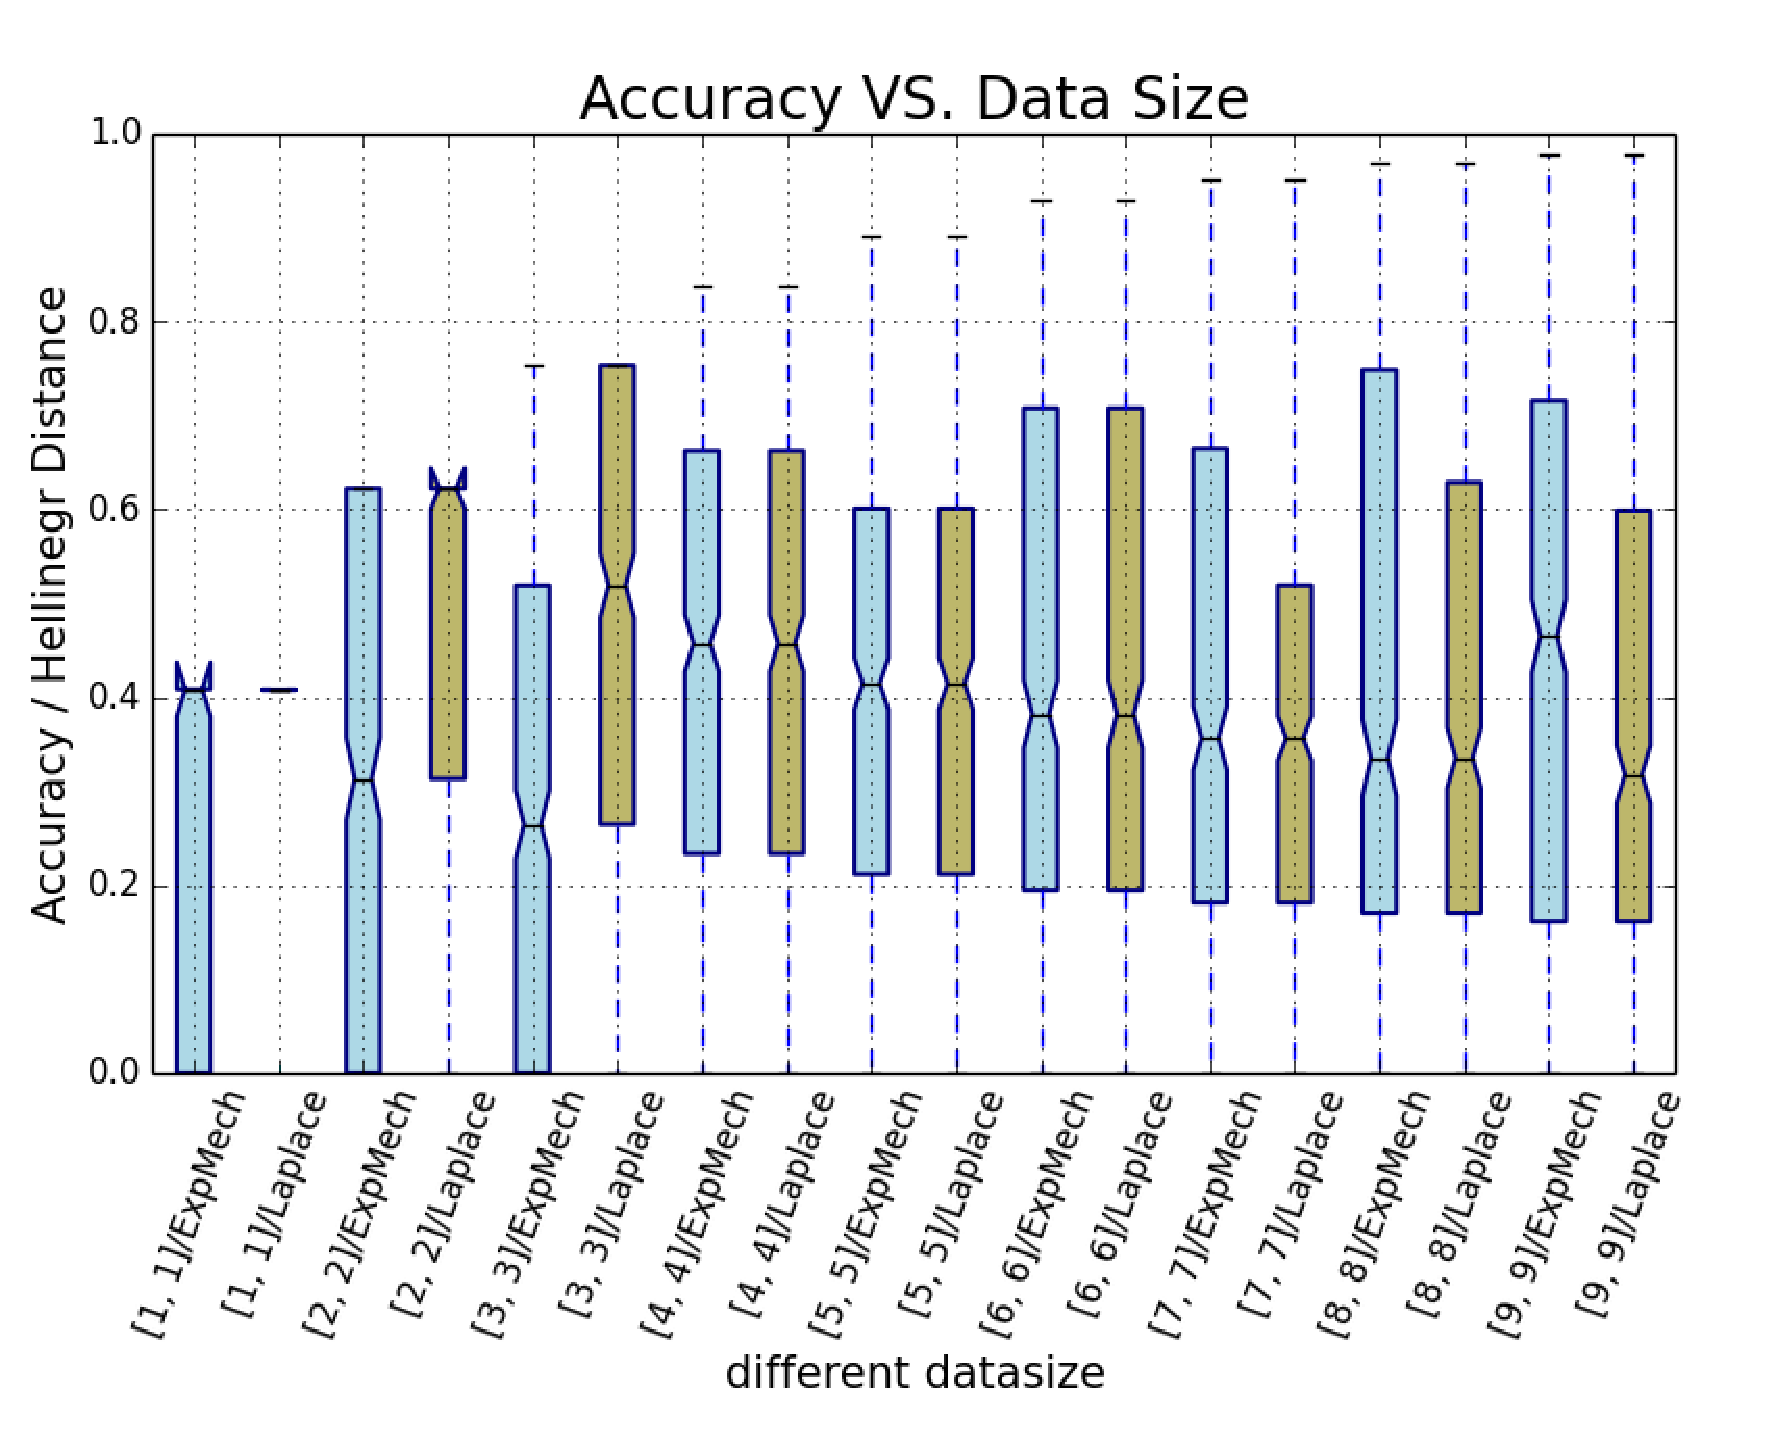
\includegraphics[width=0.3\textwidth]{accuracy_vs_datasize_1_1.eps}}
  \subfigure[three dimensions with $\dirichlet (1,1,1)$ prior distribution]{
    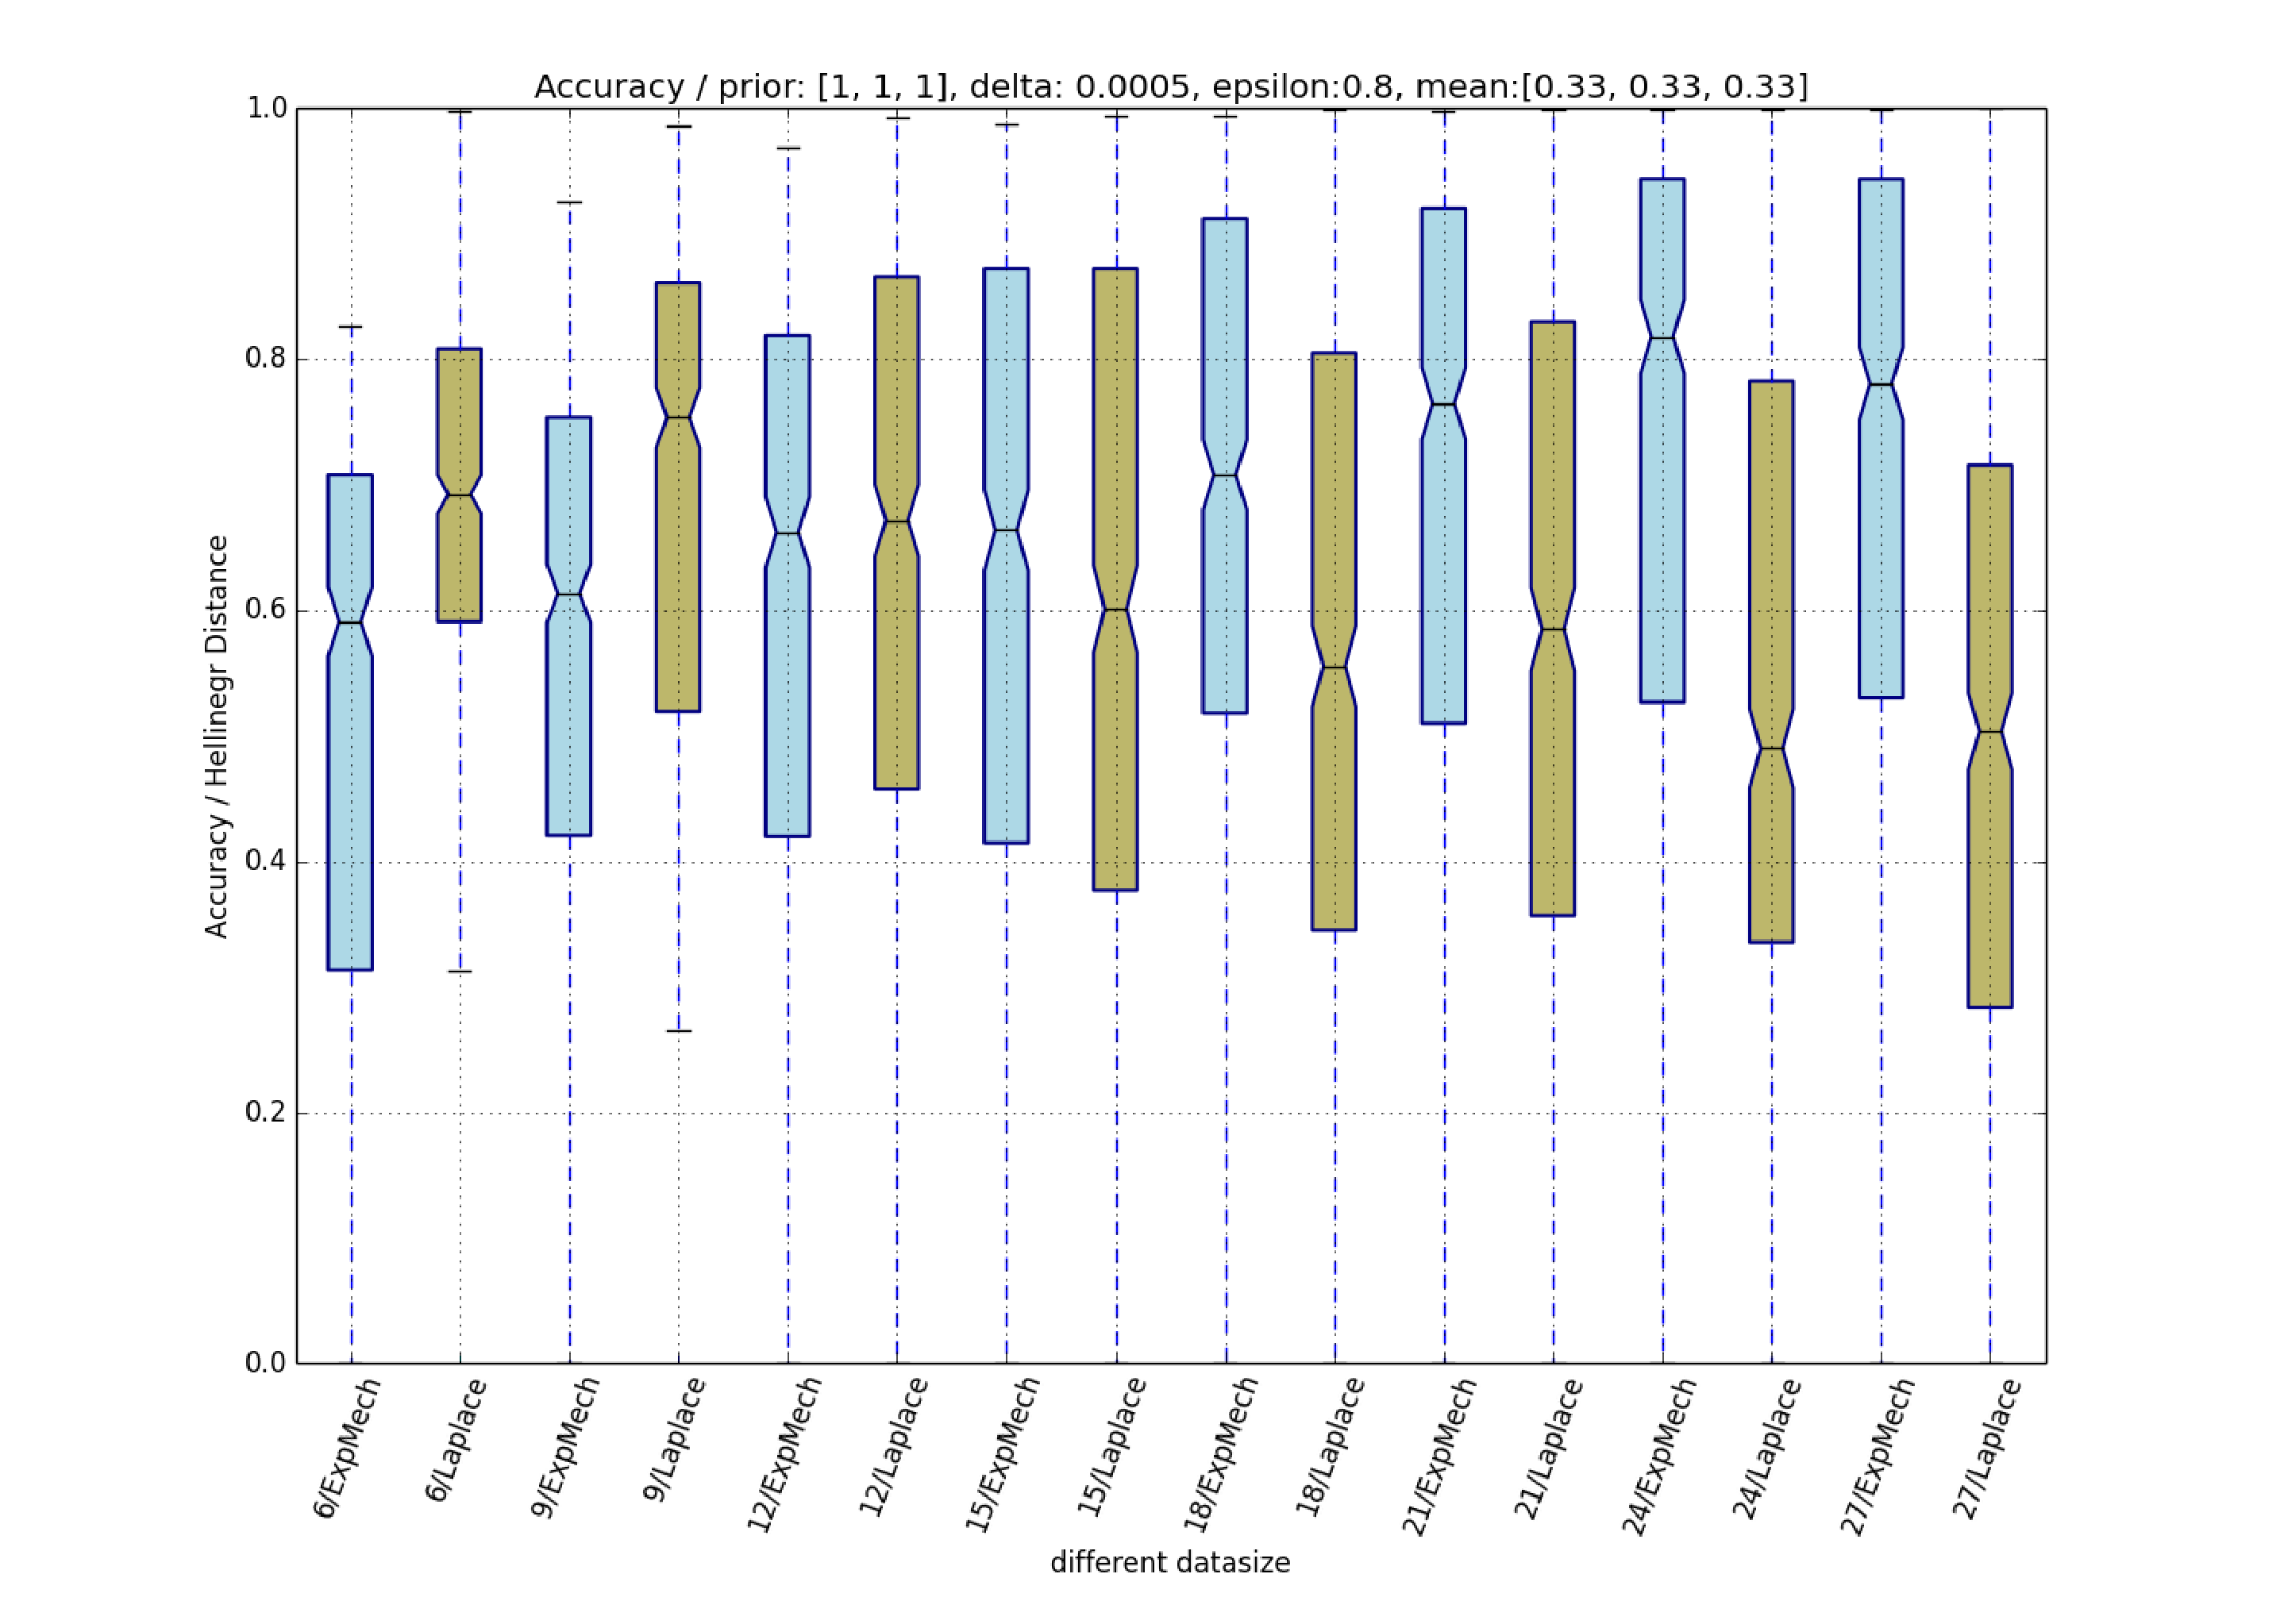
\includegraphics[width=0.3\textwidth]{accuracy_vs_datasize_1_1_1.eps}} 
\caption{Accuracy measurement based on Hellinger distance wrt. different datasizes. Settings: observed data are uniformly distributed, $\epsilon = 0.8$ and $\delta = 0.00000001$}
\label{fig_vs_datasize}
\end{center}
\end{figure}

In Fig. \ref{fig_vs_datasize}, both of the two plots show that when data size go larger, accuracy of our exponential mechanism are decreasing. In Fig. \ref{fig_vs_datasize}(a), when the data size is smaller than 12, we can beta Laplace mechanism but fail when data size larger than or equal to 12. Same as in Fig. \ref{fig_vs_datasize}(b), we can beat Laplace mechanism when data size is smaller than 15 and fail otherwise.

\subsubsection{Accuracy Evaluation wrt. Dimensions}
\label{subsubsec_vs_dimension}


\begin{figure}[ht]
\centering
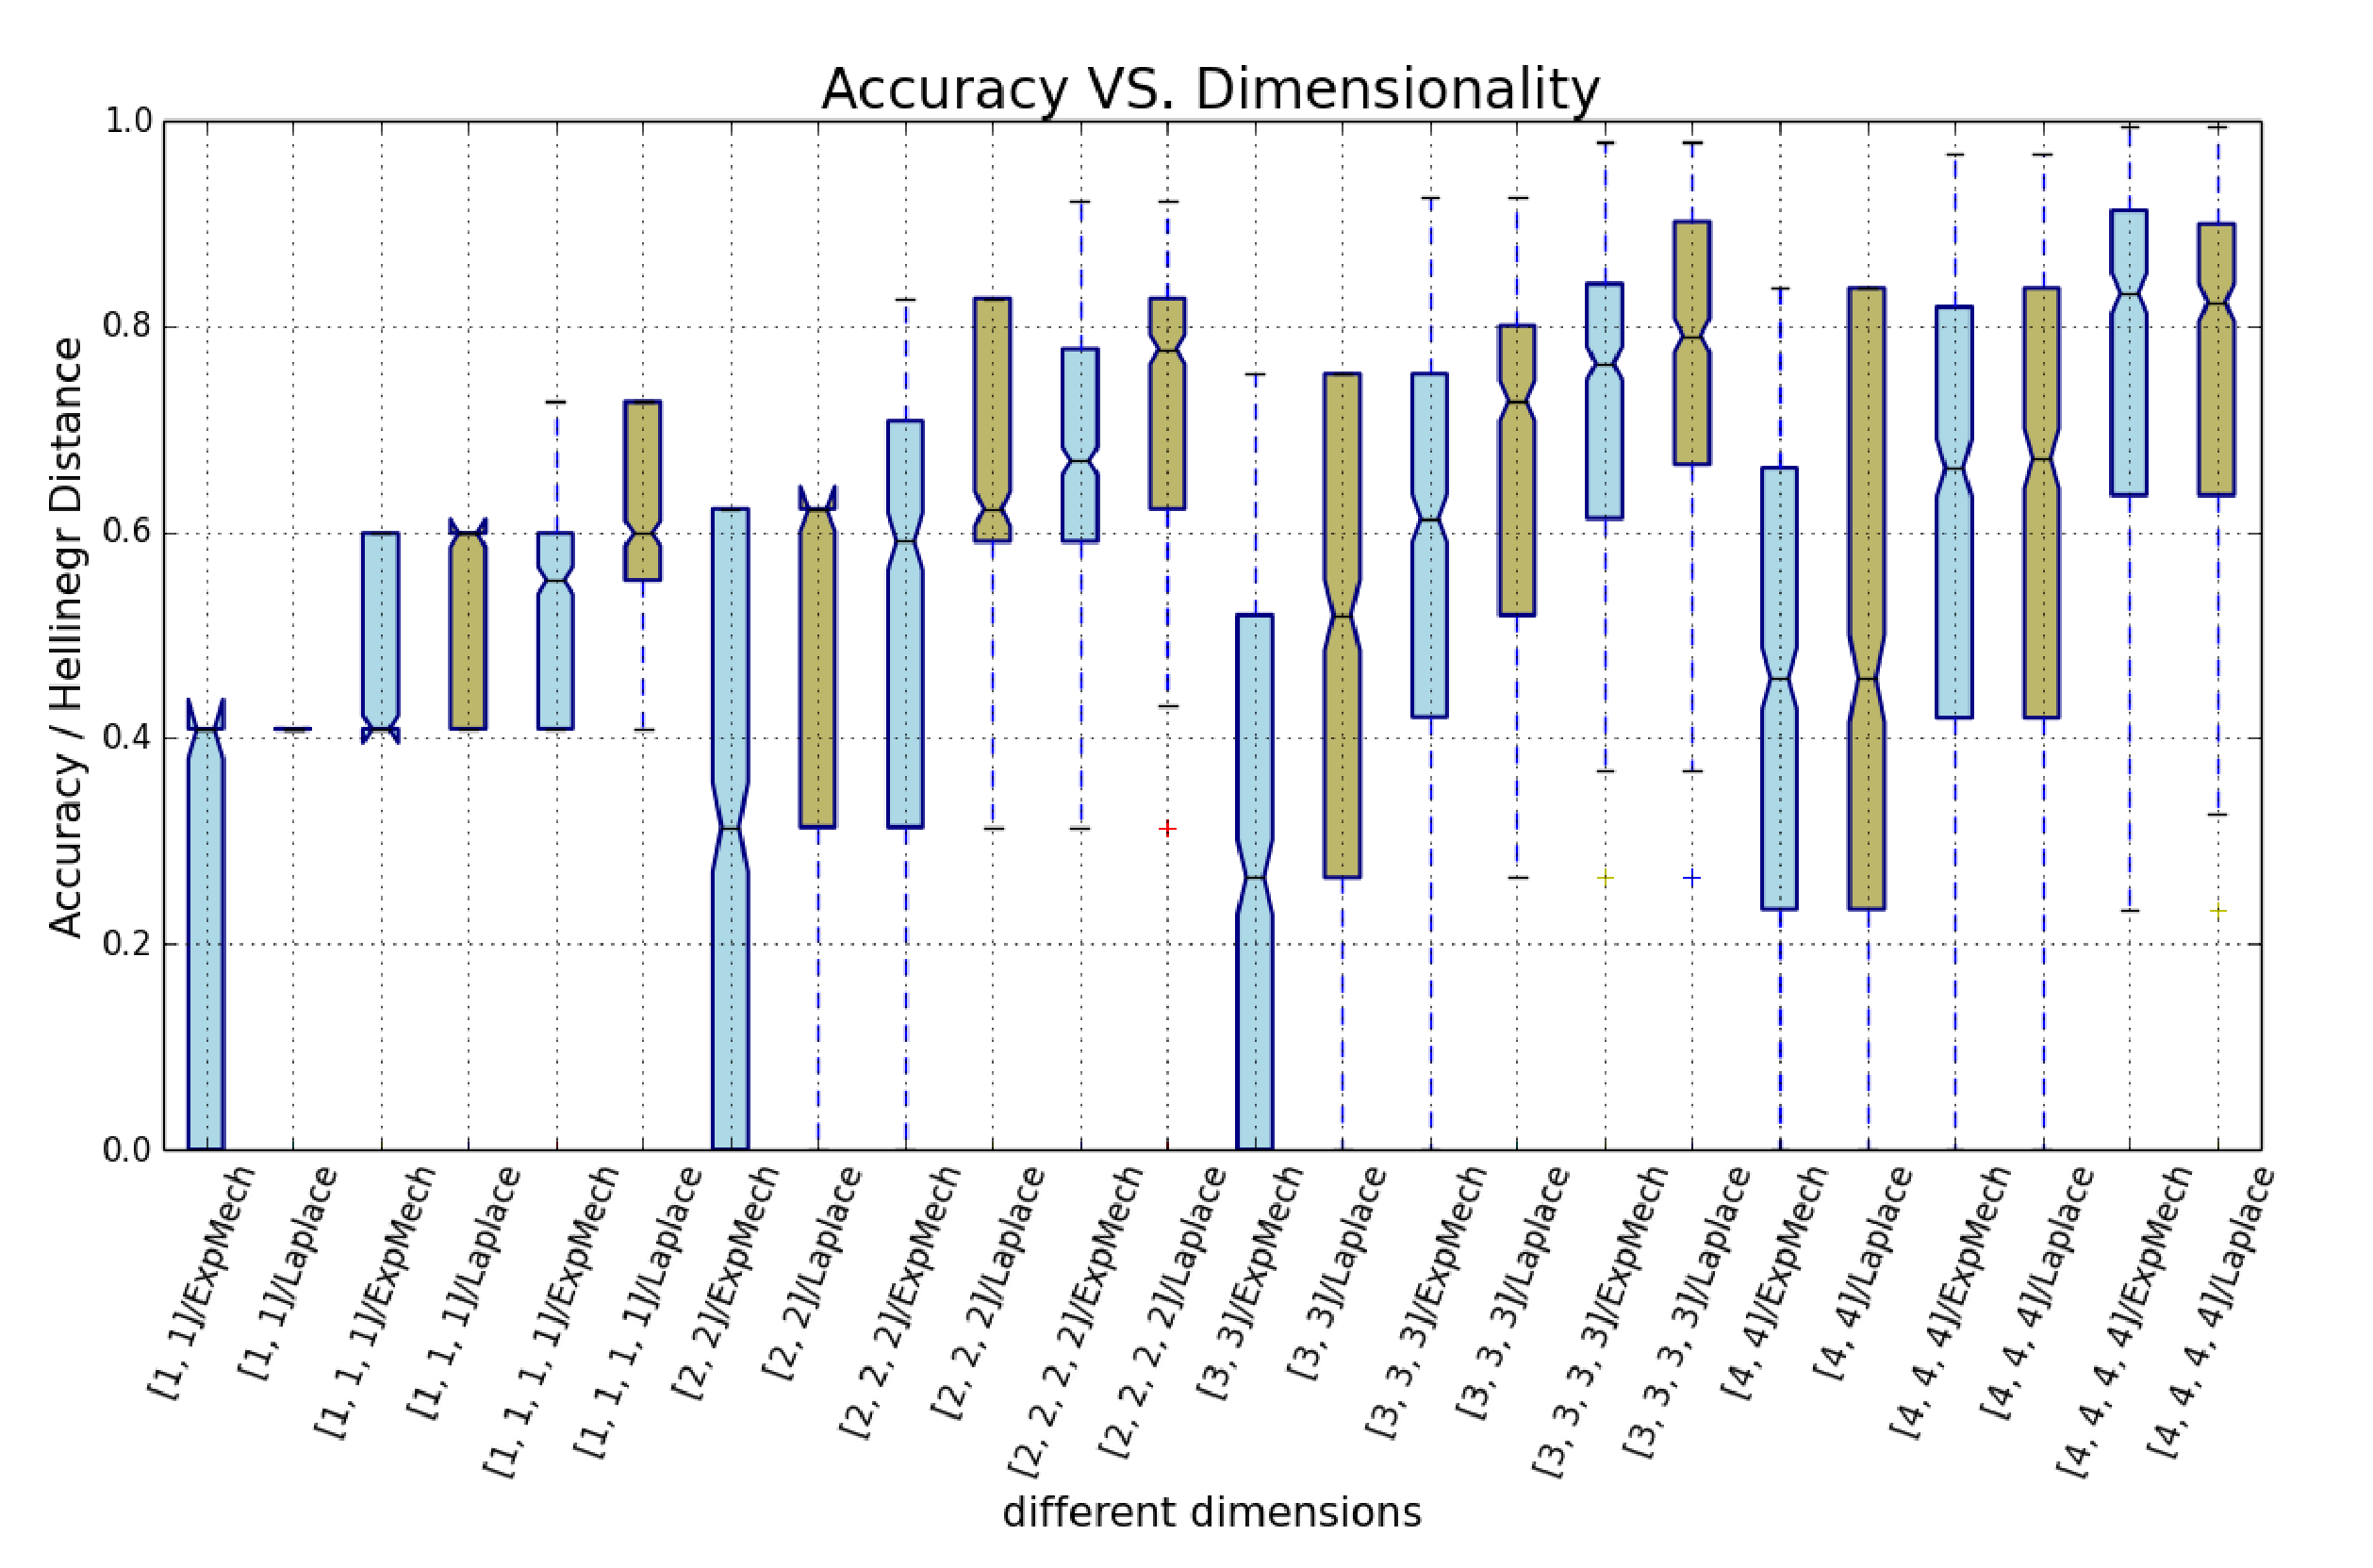
\includegraphics[width=0.45\textwidth]{accuracy_vs_dimension.eps}
\caption{Accuracy measurement based on Hellinger distance wrt. different dimensions and data size. Settings: observed data are uniformly distributed, $\epsilon = 0.8$ and $\delta = 0.00000001$, prior distributions are all $1$ in every dimension}
\label{fig_vs_dimension}
\end{figure}

In Fig. \ref{fig_vs_dimension}, x-axis are observed data sets of different size and dimensions. The plot shows that dimensions have similar influence on our exponential mechanism and the Laplace mechanism. Accuracy of two mechanisms both decrease when dimensions go larger. We will be beat by Laplace mechanism when data size increase but will not be affected when dimensions increase. In other words, dimension has little influence on whether we will beat Laplace mechanism.


\subsubsection{Accuracy Evaluation wrt. Data variance}
\label{subsubsec_vs_variance}

\begin{figure}[ht]
\centering
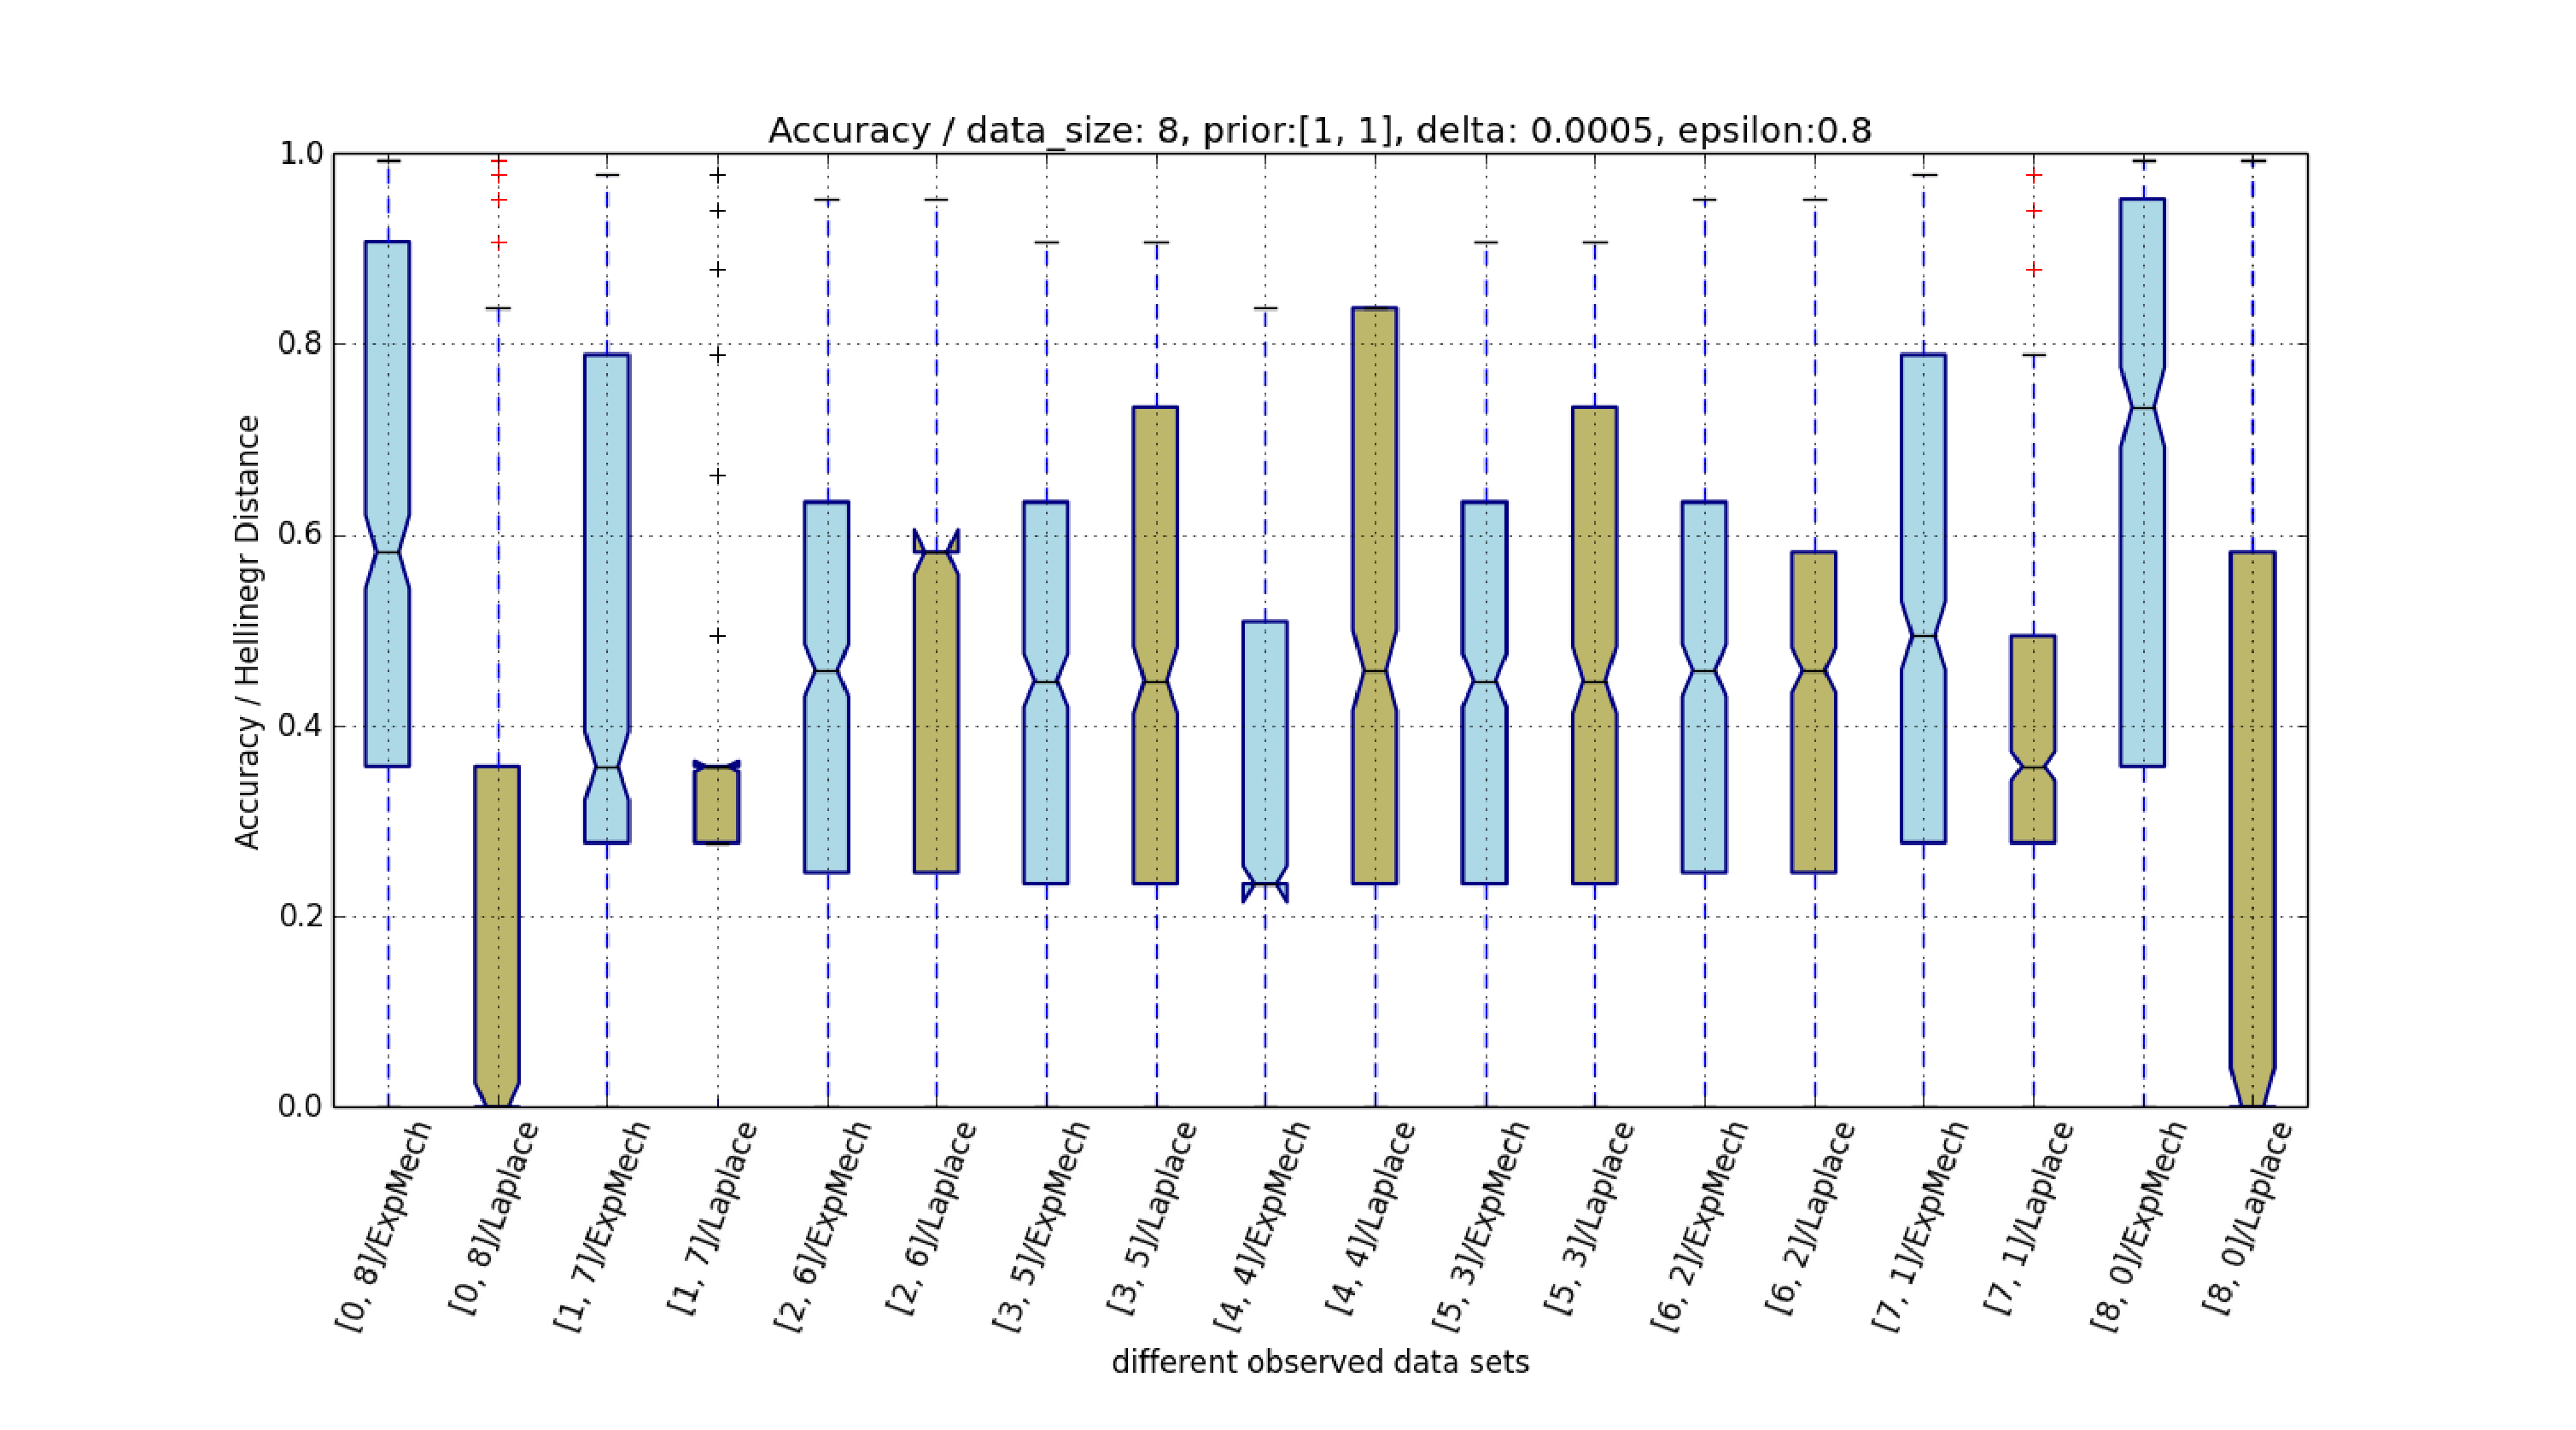
\includegraphics[width=0.45\textwidth]{accuracy_vs_mean_1_1.eps}
\caption{Accuracy measurement based on Hellinger distance wrt. different data variance. Settings: $\epsilon = 0.8$ and $\delta = 0.00000001$, prior distributions are all $1$ in every dimension}
\label{fig_vs_variance}
\end{figure}

In Fig. \ref{fig_vs_variance}, x-axis are observed data sets of different variances (or means). We study this variable under two-dimension $\betad$ distribution in order to be concise. It shows that our mechanism's accuracy is better when data variance go smaller, meanwhile Laplace mechanism go worse. We will beat Laplace mechanism when observed data are more uniformly.



\subsubsection{Accuracy Evaluation wrt. Prior Distribution}
\label{subsubsec_vs_prior}

\begin{figure}[ht]
\centering
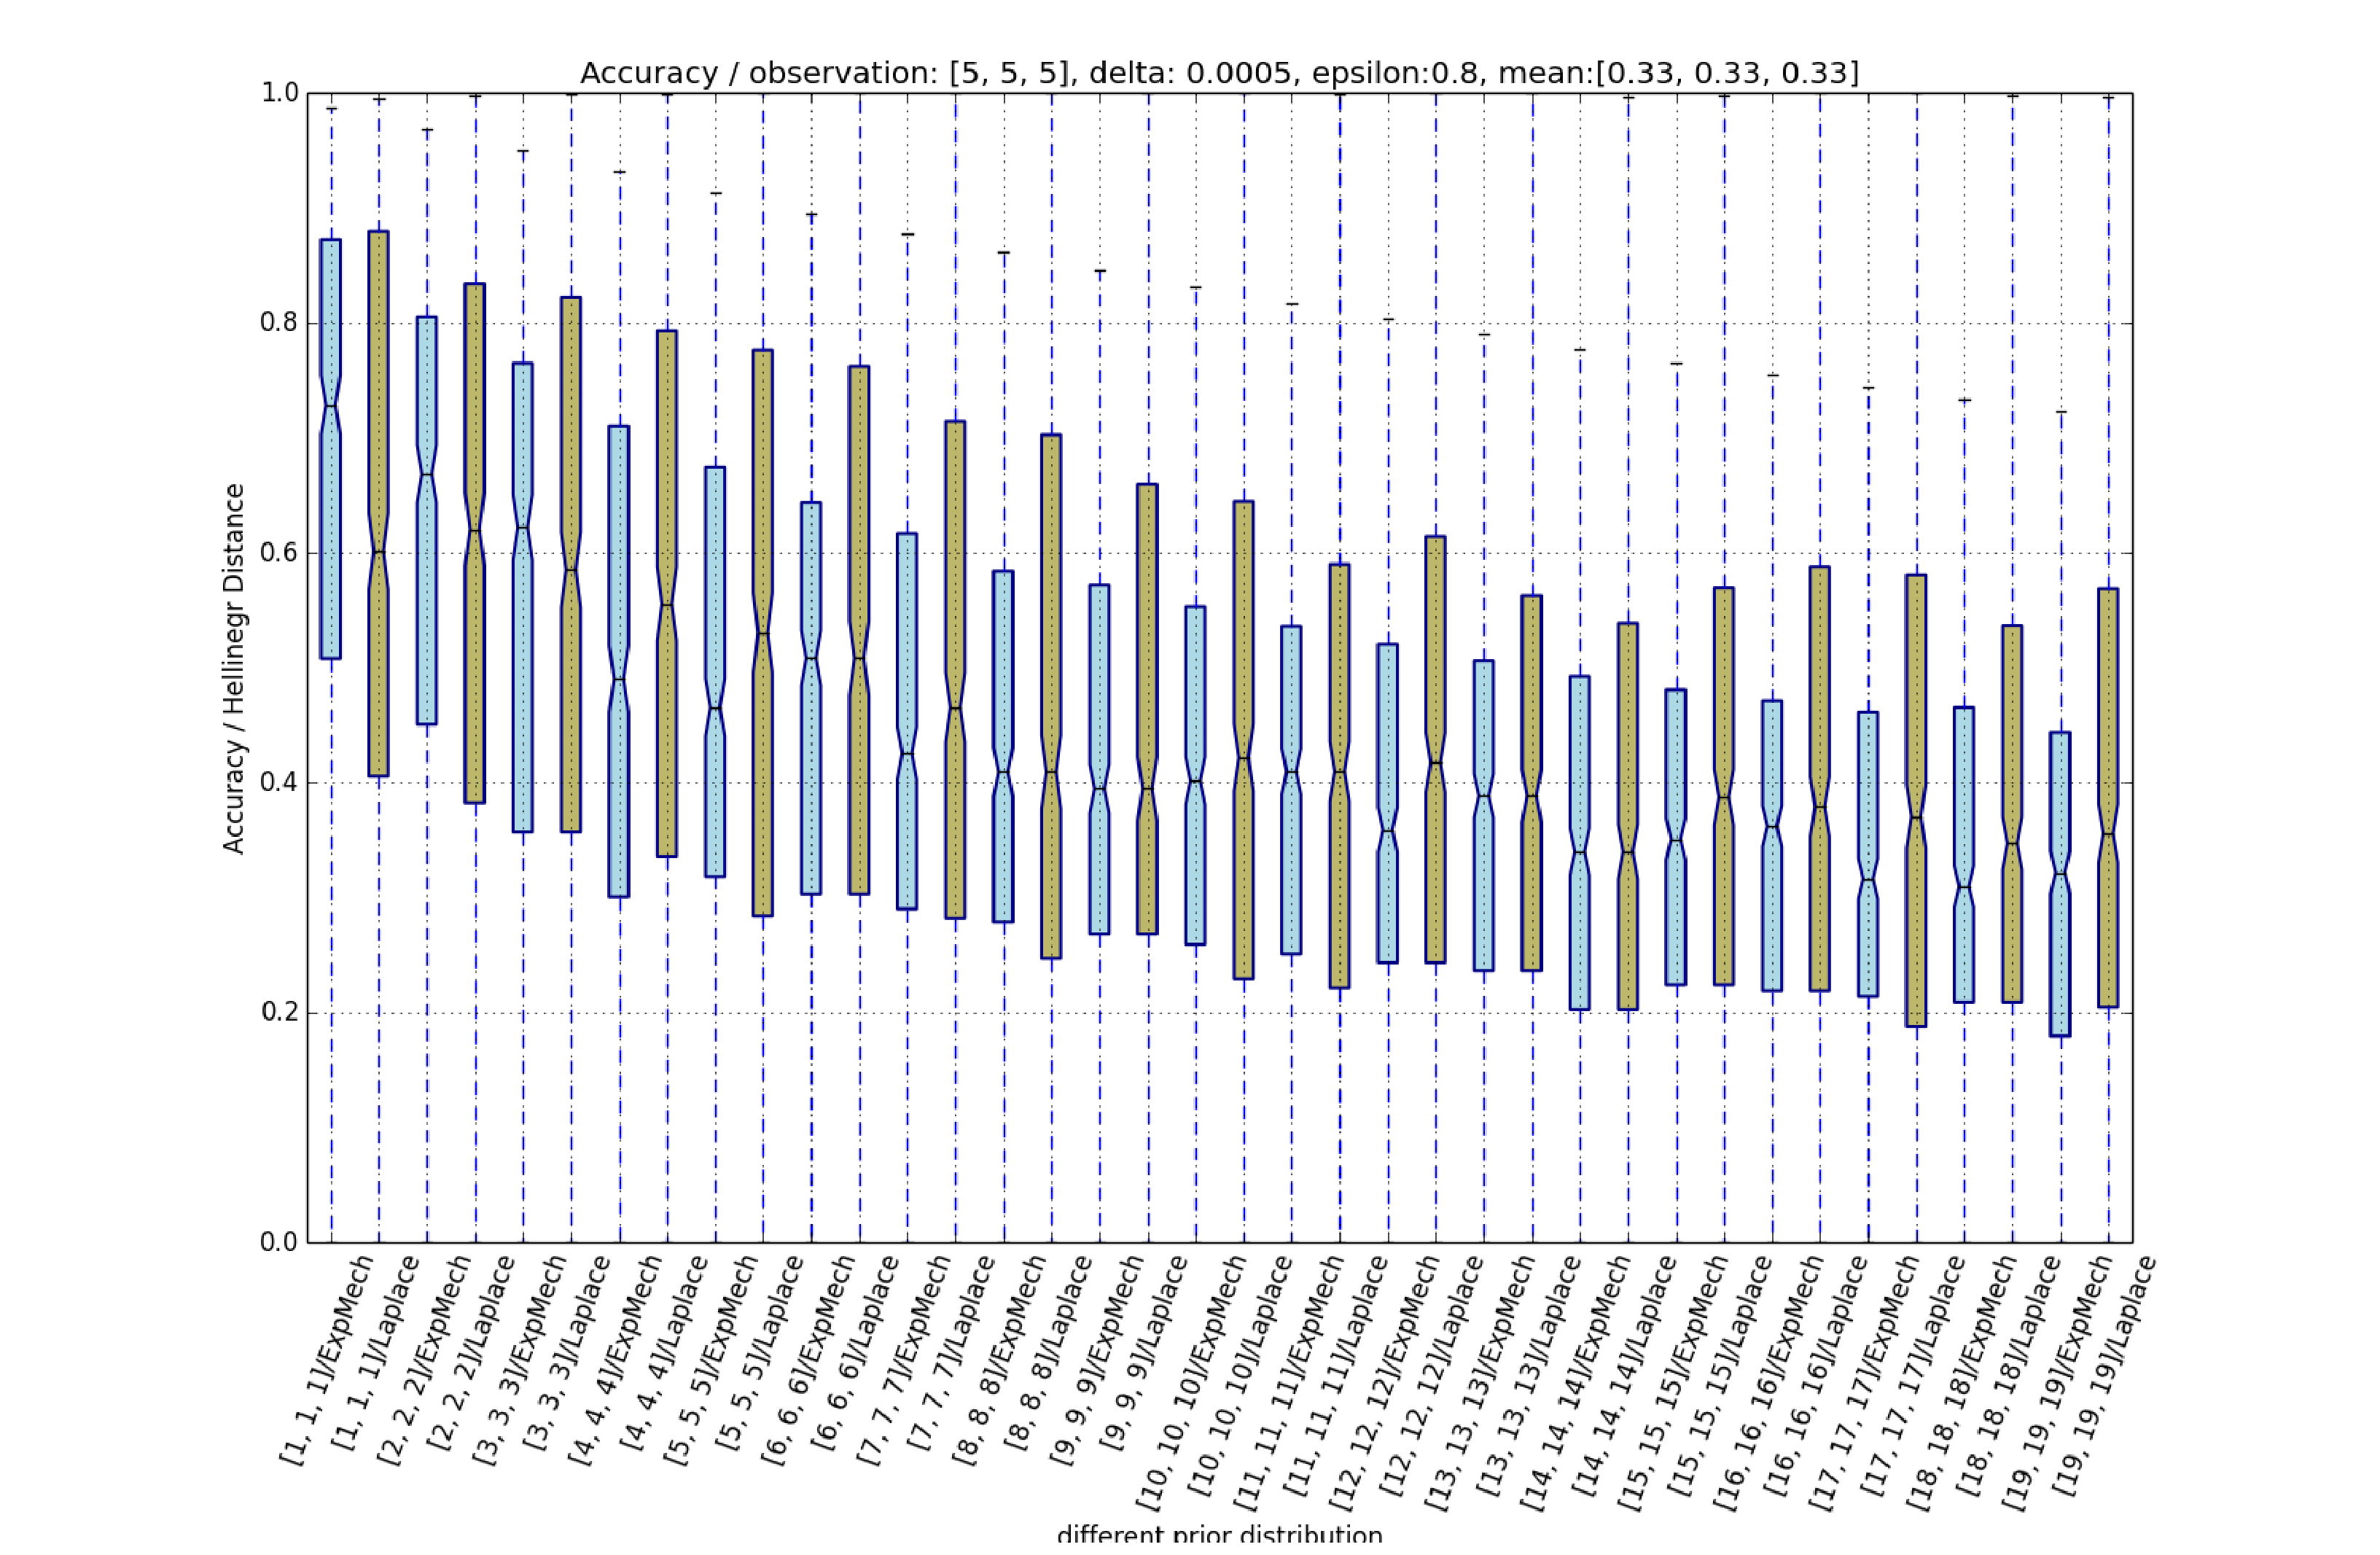
\includegraphics[width=0.45\textwidth]{accuracy_vs_prior_5_5_5.eps}
\caption{Accuracy measurement based on Hellinger distance wrt. different prior distribution. Settings: $\epsilon = 0.8$ and $\delta = 0.00000001$, observed data set is: $[5,5,5]$}
\label{fig_vs_prior}
\end{figure}

In Fig. \ref{fig_vs_prior}, we study this variable under setting that observed data set is $[5,5,5]$ because in Fig. \ref{fig_vs_datasize} Laplace mechanism beat us when data size is 15 and uniformly distributed. The plot shows that in the beginning we cannot beat Laplace but when prior distribution grow larger, we perform better and better and beat Laplace mechanism finally.



% \subsubsection{Accuracy Evaluation wrt. Prior Distribution and Data Variance}
% \label{subsubsec_vs_prior_variance}

% \begin{figure}[ht]
% \centering
% 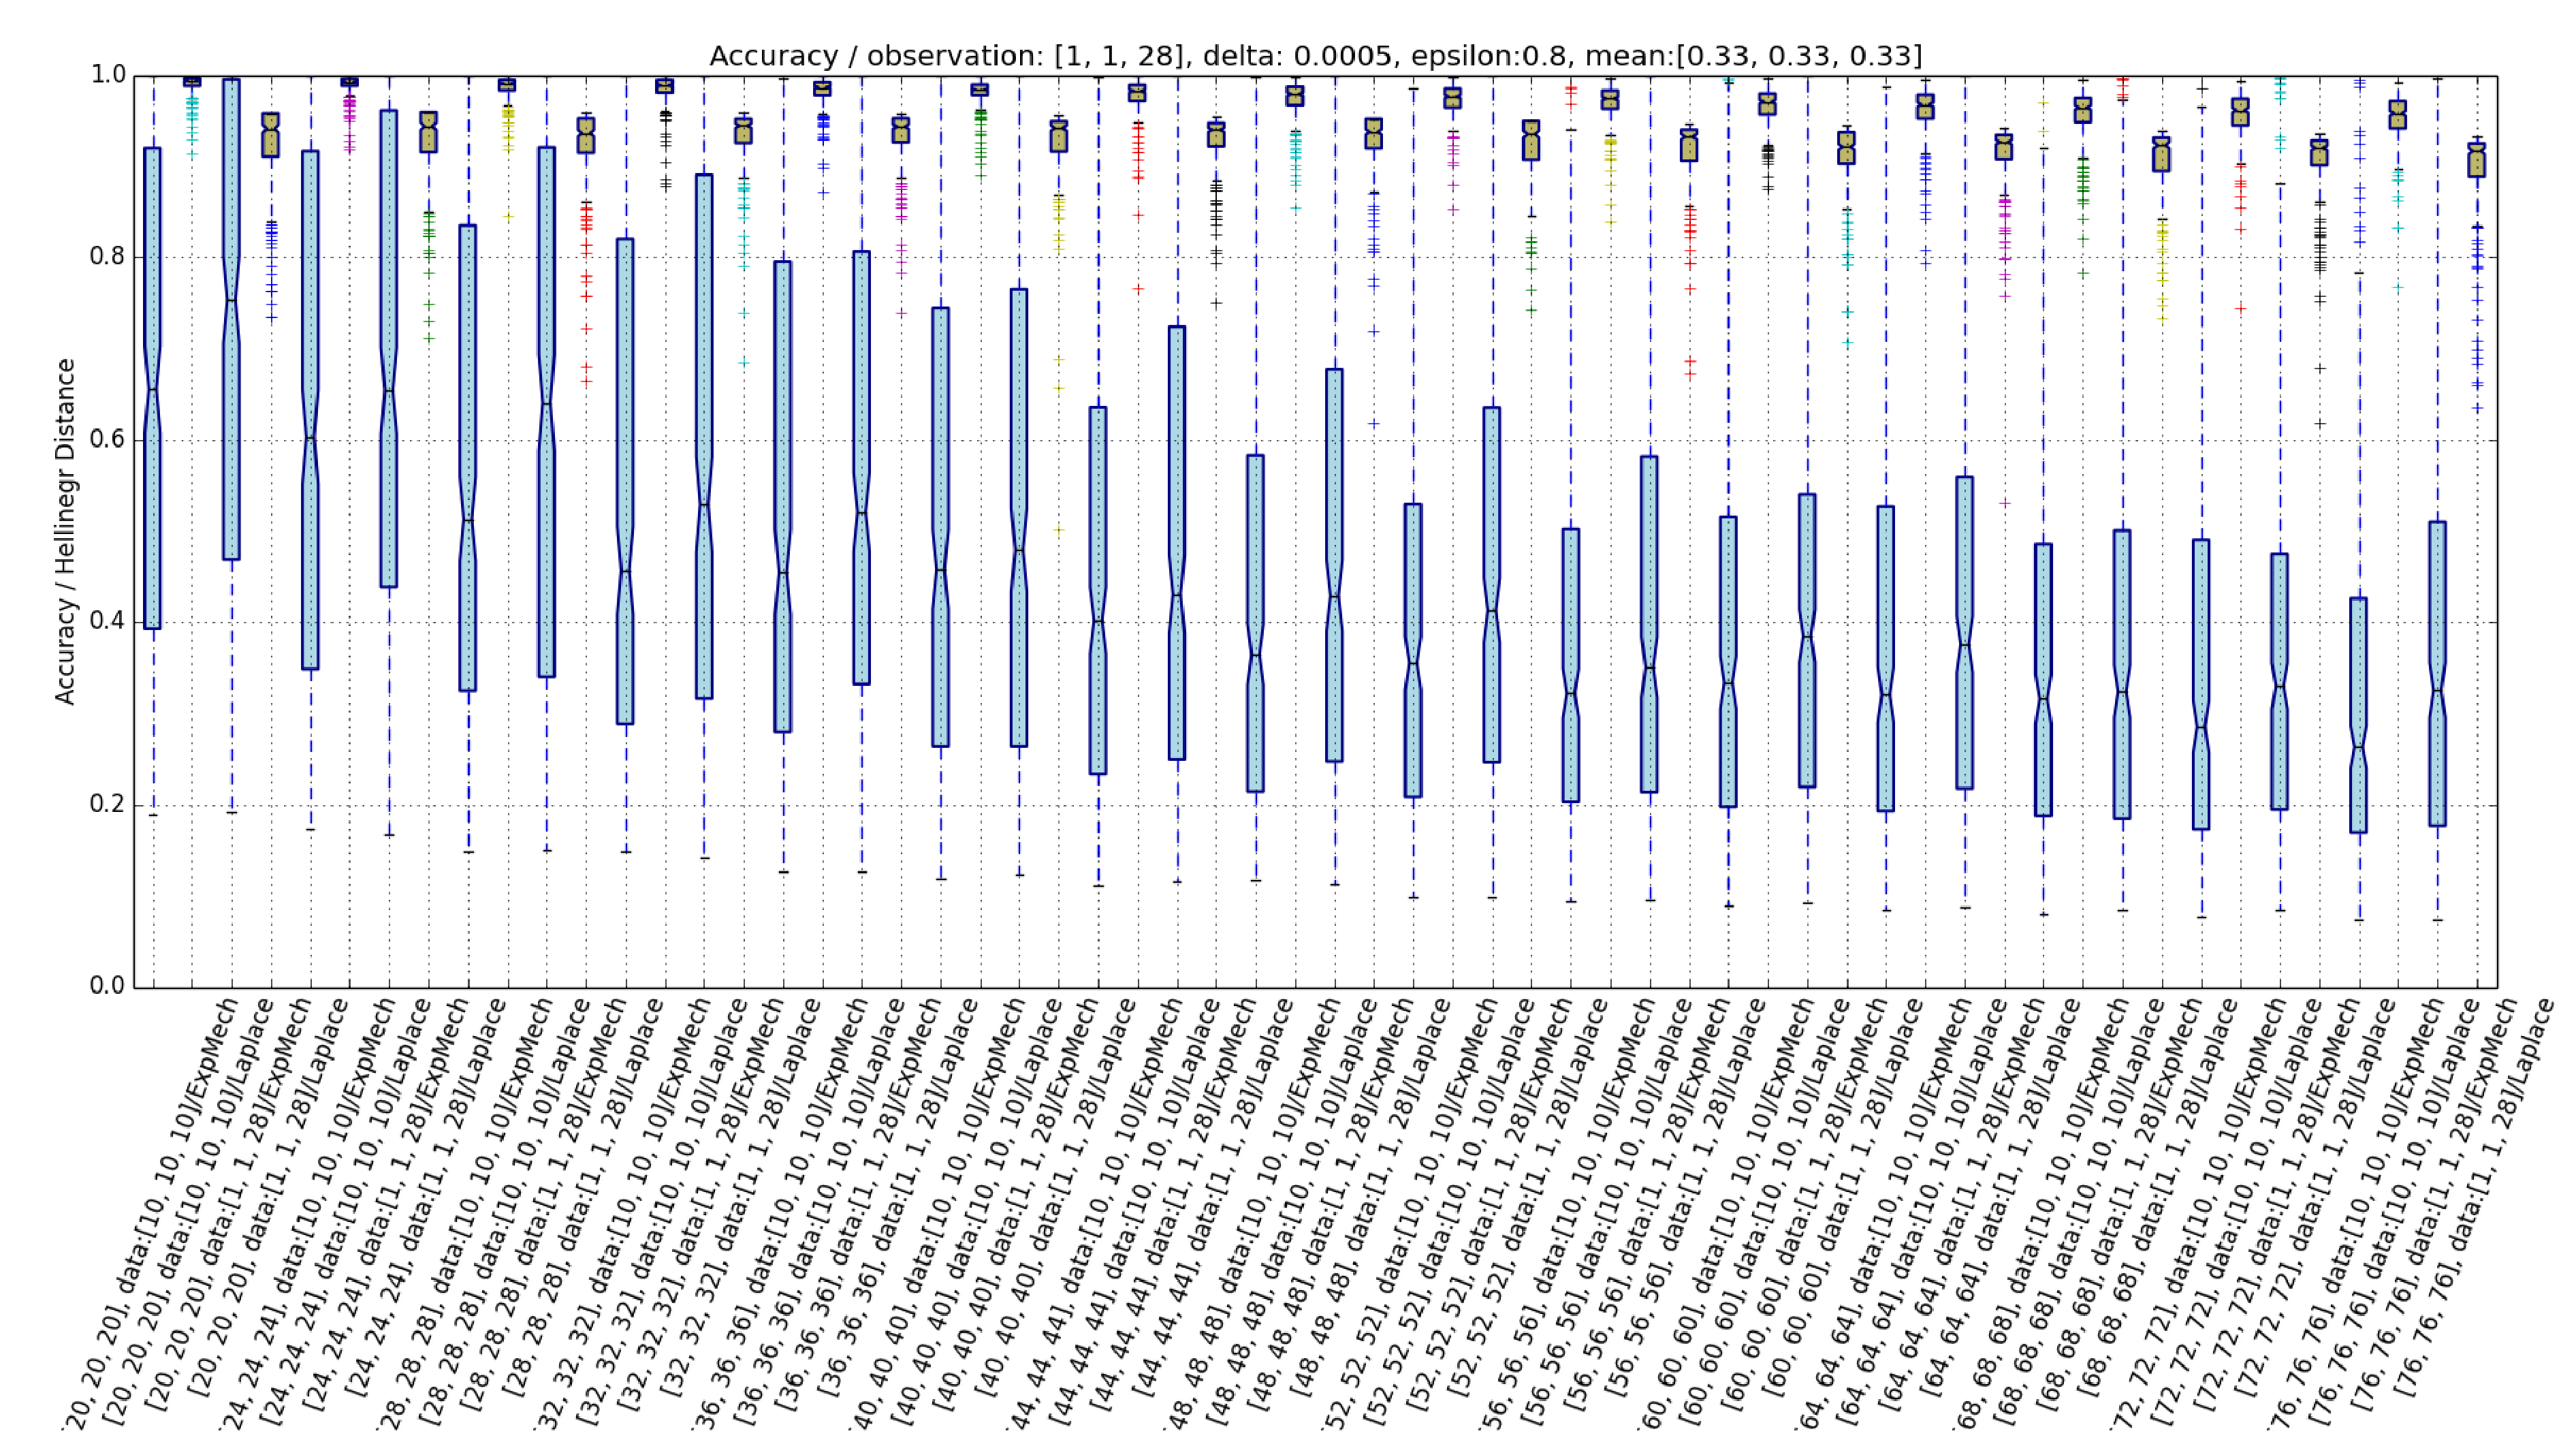
\includegraphics[width=0.45\textwidth]{Accuracy_VS_Prior_mean.eps}
% \caption{Accuracy measurement based on Hellinger distance wrt. different prior distribution and data variances. Settings: $\epsilon = 0.8$ and $\delta = 0.00000001$, observed data sets are $[10,10,10]$ and $[1,1,28]$ and prior distributions are range from $[20,20,20]$ to $[76,76,76]$}
% \label{fig_vs_prior_variance}
% \end{figure}

% Here, we change the prior distribution and data variance in the same time. As shown in Fig. \ref{fig_vs_prior_variance}, our exponential mechanism do better in uniform data set than in edging data set while Laplace mechanism on the contrary. Moreover, our mechanism is improving continuously and significantly as prior distribution increasing while Laplace mechanism isn't.


\section{Conclusions}
We can obtain some preliminary conclusions: 
\begin{enumerate}
	\item We can beat Laplace mechanism when data size is small.
	\item We will beat Laplace mechanism when observed data are more uniformly.
  \item When prior distribution grow larger, we perform better and better and beat Laplace mechanism finally.
\end{enumerate} 

In consequence, we have a better accuracy in small data size, in larger prior and in uniformly data.



\bibliographystyle{ACM-Reference-Format}
\bibliography{bayesian.bib}

\end{document}
 % TODO: replace with your brilliant paper!
% 
%packages
\usepackage{natbib}
\usepackage{amsmath}
\usepackage{amsthm}
\usepackage{mathtools}
\usepackage{mdframed}
\usepackage{subfigure}
\usepackage{booktabs}
% \usepackage{hyperref}
\usepackage{subfigure}
\usepackage{siunitx} % Provides the \SI{}{} and \si{} command for typesetting SI units
\usepackage{graphicx} % Required for the inclusion of images
% \usepackage{natbib} % Required to change bibliography style to APA
\usepackage{datetime}
\usepackage{lscape}
\usepackage{algorithm}
\usepackage{algorithmic}
\usepackage{xspace}
\usepackage[english]{babel} % English language/hyphenation
\usepackage{proof}
\usepackage{booktabs} % Top and bottom rules for tables
\usepackage[colorlinks, allcolors = blue,]{hyperref}
\usepackage{accents}
\usepackage{amsfonts}
\usepackage{stmaryrd}
\usepackage{amsmath,amsthm,amssymb,latexsym} 
\usepackage{microtype}
\usepackage{graphicx}
\usepackage{subfigure}
\usepackage{booktabs} % for professional tables
\usepackage{hyperref}
\usepackage{icml2019}
\usepackage{lipsum}

\usepackage{authblk}


%new commands
\newcommand{\theHalgorithm}{\arabic{algorithm}}
\newtheorem{definition}{Definition}
\usepackage{cancel}
\usepackage[normalem]{ulem}
\newcommand{\dataobs}{\textbf{x}}
\newcommand{\adj}[2]{\textbf{adj}(#1,#2)}
\newcommand{\candidateset}{\mathcal{R}_{\textup{post}}}
\newcommand{\bprior}{\boldsymbol{\beta}_{\textup{prior}}}
\newcommand{\bysinfer}{\mathsf{Infer}}
\newcommand{\betad}{\mathsf{Beta}}
\newcommand{\betaf}{\textup{B}}
\newcommand{\mbetaf}{\boldsymbol{\textup{B}}}
\newcommand{\vtheta}{\boldsymbol{\theta}}
\newcommand{\valpha}{\boldsymbol{\alpha}}
\newcommand{\vbeta}{\boldsymbol{\beta}}
\newcommand{\lapmech}{\mathsf{LSDim}}
\newcommand{\ilapmech}{\mathsf{LSHist}}
\newcommand{\binomial}[2]{\mathsf{Bin}(#1, #2)}
\newcommand{\multinomial}[2]{\mathsf{Mult}(#1, #2)}
\newcommand{\expmech}{\mathsf{EHD}}
\newcommand{\hexpmech}{\mathsf{EHDS}}
\newcommand{\lexpmech}{\mathsf{EHDL}}
\newcommand{\hexpmechd}{\mathsf{expMech}^{D}_{\hellinger}}
\newcommand{\privinfer}{\mathsf{PrivInfer}}
\newcommand{\hlg}{\mathsf{H}}
\newcommand{\dirichlet}[1]{\mathsf{Dir}(#1)}
\newcommand{\alphas}{\boldsymbol{\alpha}}
\newcommand{\xis}{\boldsymbol{\xi}}
\newcommand{\iverson}[1]{[#1]}
\newcommand{\datauni}{\mathcal{X}}
\newcommand{\hellinger}{\mathcal{H}}
\newcommand{\ux}[1]{u(\textbf{x}, {#1})}
\newcommand{\uxadj}[1]{u(\textbf{x}', {#1})}
\newcommand{\cardinality}[2]{\mathcal{C}^{#1}_{#2}}
\newcommand{\range}{\mathcal{O}}
\newcommand{\nomalizer}[1]{\sum\limits_{r'\in \mathcal{R}_{\textup{post}}} \exp \big(\frac{-\epsilon\cdot \mathcal{H} (\mathsf{BI}(#1),r')}{4 \cdot S(#1)}\big)}

\newcommand{\unomalizer}[1]{\sum\limits_{r'\in \mathcal{R}_{\textup{post}}} \exp \big(\frac{-\epsilon\cdot u(#1, r')}{4 \cdot S(#1)}\big)}


\newcommand{\hexpmechPr}[2]{\underset{z \thicksim \hexpmech(#1)}{\Pr}\left[ #2 \right]}
\newcommand{\lapmechPr}[2]{\underset{z \thicksim \lapmech(#1)}{\Pr}\left[ #2 \right]}

\newcommand{\ilapmechPr}[2]{\underset{
{z \thicksim \ilapmech(#1)}
}{\Pr}\left[ #2 \right]}

\newtheorem{thm}{Theorem}[section]

\newtheorem{lem}{Lemma}[section]

\newtheorem{assert}{Assertion}[lem]
\newcommand{\lap}[2]{\mathsf{Lap}(#1, #2)}
\newcommand{\todo}[1]{{\footnotesize \color{red}\textbf{[[ #1 ]]}}}

\section{Bayesian Inference Background}
Given a prior belief $\Pr(\theta)$ on some parameter $\theta$,
and given an observation $\dataobs$,
the posterior distribution on $\theta$ given $\dataobs$ is computed as:
\[
  \Pr(\theta | \dataobs) = \frac{Pr(\dataobs | \theta) \cdot \Pr(\xis)}{\Pr(\dataobs)}
\]
where the expression  $\Pr(\dataobs | \theta)$ denotes the \emph{likelihood} of $\theta$ when
\dataobs~ is observed. Since we consider \dataobs to be fixed the likelihood is a function of $\theta$.
For the same reason $\Pr(\dataobs)$ is a constant independent of $\theta$.
Usually in statistics the prior distribution $\Pr(\theta)$ is chosen so that it represents
the initial belief on $\theta$. That is, when no data has been observed. In practice though,
prior distributions and likelihood functions are usually chosen so that the posterior
belongs to the same \emph{family} of distributions. In this case we say that the prior
is conjugate of the likelihood function. Using conjugate priors simplify calculcations and allows
for inference to be performed in a recursive fashion over the data.
In this work we will consider a specific instance of Bayesian inference and one of its generalizations.
Specifically, we will consider the situation where $\theta$ represents the parameter --informally called \emph{bias})--
of a Bernoulli distributed random variable, and its immediate generalization where the parameter $\vtheta$ represents
the the vector of parameters of a categorical distributed random variable.
In the former case the prior distribution over $\theta\in [0,1]$ is going to be a beta distribution, $\betad(\alpha, \beta)$, with parameters
$\alpha,\beta\in\mathbb{R}^{+}$, and with p.d.f:
\[
  \Pr(\theta)\equiv \frac{\theta^{\alpha} (1- \theta)^{\beta}}{\betaf(\alpha,\beta)}
\]
where $\betaf(\cdot,\cdot)$ is the beta function.
The data $\dataobs$ will be a sequence of $n\in\mathbb{N}$ 0/1 values, that is $\dataobs=\ll x_1,\dots x_n \gg, x_i\in\{0,1\}$, and the likelihood function is:
\[
  \Pr(\dataobs | \theta)\equiv \theta^{a}(1-\theta)^{n-a}
\]
where $a=\displaystyle\sum_{i=1}^{n}\mathrm{x_i}$.
From this it can easily be derived that the posterior distribution is:
\[
  \Pr(\theta|\dataobs)=\betad(\alpha+a,\beta+n-a)
\]
In the latter case the prior distribution over $\vtheta\in [0,1]^{k}$ is given by a Dirichelet distribution, $\dirichlet(\vtheta)$, for $k\in\mathbf{N}$,
and $\valpha\in(\mathbf{R^{+}})^{k}$, with p.d.f:
\[
  \Pr(\vtheta)\equiv\frac{1}{\mbetaf(\valpha)}\cdot \displaystyle\prod_{i=1}^{k}{\theta_i^{\alpha_i-1}}
\]
where $\mbetaf(\cdot)$ is the generealised beta function.
The data $\dataobs$ will be a sequence of $n\in\mathbb{N}$ values coming from a universe $\datauni$, such that $\mid\datauni \mid=k$.
The likelihood function will be:
\[
  \Pr(\dataobs|\vtheta)\equiv \displaystyle\prod_{a\in\datauni}\alpha_{a}^{z_a}
\todo{to check}\]
where $z_a=\displaystyle\sum_{i=1}^{n}\iverson{x_i=a}$, where in $\iverson{\cdot}$ we use
Iverson bracket notation. The posterior distribution over $\vtheta$ turns out to be
\[
  \Pr(\vtheta|\dataobs)=\todo{to type down}\dirichlet(\vtheta+...)
\]
\section{Problem Statement}
% When we try
% to make this distribution public, sensitive information of the data
% based on which the posterior drew from can be compromised. So, it is
% important to protect this posterior distribution. When our protection
% objective is a distribution rather than a numeric value or vector, it
% would be better to measure the accuracy by distance over
% distributions, for instance, Hellinger distance, than by numeric
% metrics like $\ell_1$-norm.
This work will show that the same mechanism can
perform differently when its accuracy is computed w.r.t to a metric
over probability measures (e.g total variation distance, or Hellinger distance)
from when the metric (e.g. $\ell_1$-norm) is over the parameters.  
\section{Technical Problem Statement}
\label{sec_bayesInfer}
The posterior belief about parameters $\xis$ is inferred from the
group of sensitive data. Because it is usually published in form of a
distribution, for example, $\betad(\alpha',\beta'), \cdots,$ itself
can relieve a lot of information about sensitive data. So, the
sensitive information we want to protect here is the posterior belief,
i.e., $Pr(\xis | \dataobs)$, rather than just a sample drew from
it\cite{foulds2016theory}. Then it will be better if we can use a
distance over two distributions to measure the accuracy than a
distance over just parameters or values when we are protecting a
distribution, for instance, Hellinger distance in our paper. When we
measure the accuracy between true posterior and protected posterior
using Hellinger distance, it would be better we can have a protection
mechanism based on Hellinger distance. However, current mechanisms are
mainly based on $l_1$ norm by Laplace mechanism
\cite{zhang2016differential} \cite{xiao2012bayesian}. That's why we
design our exponential mechanism over Hellinger distance to protect
the whole posterior distribution.


\section{Baseline Approach - Laplace Mechanism}
\label{sec_lap}
Based on the posterior results from Bayesian inference, we calculate the Laplace mechanism updates on posterior and get the private results under Laplace mechanism. In the case of $m$ dimension Dirichlet distribution, we will add $(m-1)$ i.i.d. Laplace noises $\{| Lap_1 |, | Lap_2 |, \cdots, | Lap_{m-1} |\}$ to the output, where $Lap_i = floor(Y)$, $Y \sim Lap(\frac{2}{\epsilon})$. The private posterior then will be $\dirichlet(\alpha_1 + n_1 + | Lap_1 |, \alpha_2 + n_2 + | Lap_2 |, \cdots, \alpha_m + n - (Lap_1 + \cdots + Lap_{m-1}))$.

\section{Our Approach - Exponential Mechanism with Smooth Sensitivity}
\label{sec_smoo}

% \subsection{Algorithm Setting up}
We define a new mechanism $\hexpmech(x)$ which is similar to the exponential mechanism where we use $\mathcal{R}$ as the set $\betaset$ of beta distributions with integer parameters summing up to $n+2$, as scoring function we use the Hellinger distance from $\bysinfer(x)$, i.e. $\hlg(\bysinfer(x),-)$, and we calibrate the noise to the smooth sensitivity~\cite{nissim2007smooth}. The only difference is in the sensitivity part, since now we use the smooth sensitivity.

\begin{definition}
\label{def_smoo}
The mechanism $\hexpmech(x)$ outputs a candidate $r \in \betaset$ with probability
\begin{equation*}
\underset{z \thicksim \hexpmech(x)}{Pr}[z=r] = \frac
{exp(\frac{-\epsilon\hlg(\bysinfer(x),r)}{2 S_\beta(x)})}
{\Sigma_{r' \in R}\ exp(\frac{-\epsilon \hlg(\bysinfer(x),r')}{2 S_\beta(x)})},
\end{equation*}
where $s_\beta(x)$ is the smooth sensitivity of $\hlg(\bysinfer(x),-)$, calculated by:
\begin{equation*}
S_{\beta}(x) = \max(\Delta_{l}\hlg(\bysinfer(x),-), \max_{y \neq x; y \in D^{n}}(\Delta_{l}\hlg(\bysinfer(y),-)\cdot e^{-\beta d(x,y)})),
\end{equation*}
where $d$ is the Hamming distance between two datasets, and $\beta =
\beta(\epsilon, \delta)$ is a function of $\epsilon$ and $\delta$. 
\end{definition}


In what follows, we will use a correspondence between the probability
 $\underset{z \thicksim \hexpmech(x)}{Pr}[z = r]$ of every
 $r\in\betaset$ and the probability 
 $\underset{z \thicksim \hexpmech(x)}{Pr}[\hlg(\bysinfer(x),z) =
 \hlg(\bysinfer(x),r)]$ for the utility score for $r$. In particular, for every
 $r\in\betaset$ we have:
$$
\underset{z \thicksim \hexpmech(x)}{Pr}[z = r]=
\frac{1}{2}\Big (\underset{z \thicksim \hexpmech(x)}{Pr}[\hlg(\bysinfer(x),z) =
 \hlg(\bysinfer(x),r)]\Big )
$$
To see this, it is enough to notice that: $\underset{z \thicksim \hexpmech(x)}{Pr}[z = r]$ is proportional too $\hlg(\bysinfer(x),r)$, i.e., $u(x,z)$. We can derive, if $u(r,x) = u(r',x)$ then $\underset{z \thicksim \hexpmech(x)}{Pr}[z = r] = \underset{z \thicksim \hexpmech(x)}{Pr}[z = r']$. We assume the number of candidates $z \in \mathcal{R}$ that satisfy $u(z,x) = u(r,x)$ is $|r|$, we have  $\underset{z \thicksim \hexpmech(x)}{Pr}[u(z,x) = u(r,x)] = |r| \underset{z \thicksim \hexpmech(x)}{Pr}[z = r]$. Because Hellinger distance  $\hlg(\bysinfer(x),z)$ is axial symmetry, where the $\bysinfer(x)$ is the symmetry axis. It can be infer that $|z| = 2$ for any candidates, apart from the true output, i.e., $\underset{z \thicksim \hexpmech(x)}{Pr}[u(z,x) = u(r,x)] = 2 \underset{z \thicksim \hexpmech(x)}{Pr}[z = r]$. This parameter can be eliminate in both sides in proof.

In our private Bayesian inference mechanism, we set the $\beta$ as $\ln(1 - \frac{\epsilon}{2 \ln (\frac{\delta}{2 (n + 1)})})$. 





% \subsection{Sliding Property of Exponential Mechanism}
% \begin{lem}
% Consider the exponential mechanism  $\sexpmech(x,u,\mathcal{R})$
% calibrated on the smooth sensitivity. Let $\lambda = f(\epsilon,
% \delta)$, $\epsilon\geq 0$ and $|\delta| < 1$. Then, the following \emph{sliding property} holds:
% \begin{equation*}
% \underset{r \thicksim \hexpmech(x)}{Pr}[u(r,x) = \hat{s}]
% \leq
% e^{\frac{\epsilon}{2}} \underset{r \thicksim \hexpmech(x)}{Pr}[u(r,x) = (\Delta + \hat{s})] + \frac{\delta}{2},
% \end{equation*}

% \end{lem}

% \begin{proof}

% We denote the normalizer of the probability mass in $\hexpmech(x)$: $\sum_{r' \in \mathcal{R}}exp(\frac{\epsilon u(r',x)}{2 S(x)})$ as $NL(x)$:
% \begin{equation*}
% \begin{split}
% LHS 
%   = \underset{r \thicksim \hexpmech(x)}{Pr}[u(r,x) = \hat{s}]
% & = \frac{exp(\frac{\epsilon \hat{s}}{2 S(x)})}{NL(x)}\\
% & = \frac{exp(\frac{\epsilon (\hat{s} + \Delta - \Delta)}{2 S(x)})}{NL(x)}\\
% & = \frac{exp(\frac{\epsilon (\hat{s} + \Delta)}{2 S(x)} + \frac{- \epsilon \Delta}{2 S(x)})}{NL(x)}\\
% & = \frac{exp(\frac{\epsilon (\hat{s} + \Delta)}{2 S(x)})}{NL(x)} \cdot e^{\frac{- \epsilon \Delta}{2 S(x)})}.\\
% \end{split}
% \end{equation*}

% By bounding the $\Delta \geq -S(x)$, we can get:

% \begin{equation*}
% \begin{split}
% \frac{exp(\frac{\epsilon (\hat{s} + \Delta)}{2 S(x)})}{NL(x)} \cdot e^{\frac{- \epsilon \Delta}{2 S(x)}}
% & \leq \frac{exp(\frac{\epsilon (\hat{s} + \Delta)}{2 S(x)})}{NL(x)} \cdot e^{\frac{\epsilon}{2}}\\
% &  =  e^{\frac{\epsilon}{2}} \underset{z \thicksim \hexpmech(x)}{Pr}[u(r,x) = (\Delta + \hat{s})] \leq RHS\\
% \end{split}
% \end{equation*}

% \end{proof}

% \subsection{Dilation Property of Exponential Mechanism}
% \begin{lem}
% for any exponential mechanism $\hexpmech(x)$, $\lambda < |\beta|$, $\epsilon$, $|\delta| < 1$ and $\beta \leq \ln(1 - \frac{\epsilon}{2 \ln (\frac{\delta}{2 (n + 1)})})$, the dilation property holds:

% \begin{equation*}
% \underset{z \thicksim \hexpmech(x)}{Pr}[u(z,x) = c]
% \leq
% e^{\frac{\epsilon}{2}} \underset{z \thicksim \hexpmech(x)}{Pr}[u(z,x) = e^{\lambda} c] + \frac{\delta}{2},
% \end{equation*}
% where the sensitivity in mechanism is still smooth sensitivity as above.
% \end{lem}

% \begin{proof}

% The sensitivity is always greater than 0, and our utility function $-\hlg(\bysinfer(x),z)$ is smaller than zero, i.e., $u(z,x) \leq 0$, we need to consider two cases where $\lambda < 0$, and $\lambda > 0$:

% We set the $h(c) = Pr[u(\hexpmech(x)) = c] = 2\frac{exp(\frac{\epsilon z}{2 S(x)})}{NL(x)}$.

% We first consider $\lambda < 0$. In this case, $1 < e ^ {\lambda}$, so the ratio $\frac{h(c)}{h(e^{\lambda}c)} = \frac{exp(\frac{\epsilon c}{2 S(x)})}{exp(\frac{\epsilon (c \cdot e^{\lambda})}{2 S(x)})}$ is at most $\frac{\epsilon}{2}$.

% Next, we proof the dilation property for $\lambda > 0$, The ratio of $\frac{h(c)}{h(e^{\lambda}c)}$ is $\exp(\frac{\epsilon}{2} \cdot \frac{u(\hexpmech(x)) (1 - e^{\lambda})}{S(x)})$. Consider the event $G = \{ \hexpmech(x) : u(\hexpmech(x)) \leq \frac{S(x)}{(1 - e^{\lambda})}\}$. Under this event, the log-ratio above is at most $\frac{\epsilon}{2}$. The probability of $G$ under density $h(c)$ is $1 - \frac{\delta}{2}$. Thus, the probability of a given event $z$ is at most $Pr[c \cap G] + Pr[\overline{G}] \leq e^{\frac{\epsilon}{2}} Pr[e^{\lambda}c \cap G] + \frac{\delta}{2} \leq e^{\frac{\epsilon}{2}} Pr[e^{\lambda}c] + \frac{\delta}{2}$.\\


% \textbf{Detail proof:}
% \begin{itemize}

% 	\item $\lambda < 0$

% 		The left hand side will always be smaller than 0 and the right hand side greater than 0. This will always holds, i.e.
% 		\begin{equation*}
% 		\end{equation*}
% 	\item $\lambda > 0$


% Because $\hat{s} = u(r)$ where $r \thicksim \hexpmech(x)$, we can substitute $\hat{s}$ with $u(\hexpmech(x))$. Then, what we need to proof under the case $\lambda > 0$ is:
% \begin{equation*}
% u(\hexpmech(x)) \leq \frac{S(x)}{(1 - e ^ {\lambda})}
% \end{equation*}
% By applying the accuracy property of exponential mechanism, we bound the probability that the equation holds with probability:
% \begin{equation*}
% \begin{split}
% Pr[u(\hexpmech(x)) \leq \frac{S(x)}{(1 - e ^ {\lambda})}] 
% & \leq \frac{|\mathcal{R}|exp(\frac{\epsilon S(x)}{(1 - e ^ {\lambda})}/2 S(x))}{|\mathcal{R}_{OPT}| exp(\epsilon OPT_{u(x)}/2 S(x))}\\
% \end{split}
% \end{equation*}

% In our Bayesian Inference mechanism, the size of the candidate set $\mathcal{R}$ is equal to the size of observed data set plus 1, i.e., $n + 1$, and $OPT_{u(x)} = 0$, then we have:
% \begin{equation*}
% \begin{split}
% Pr[u(\hexpmech(x)) \leq \frac{S(x)}{(1 - e ^ {\lambda})}] 
% & = (n + 1)exp(\frac{\epsilon S(x)}{(1 - e ^ {\lambda})}/2 S(x))\\
% & = (n + 1)exp(\frac{\epsilon}{2 (1 - e ^ {\lambda})})\\
% \end{split}
% \end{equation*}

% When we set $\lambda \leq \ln(1 - \frac{\epsilon}{2 \ln (\frac{\delta}{2 (n + 1)})})$, it is easily to derive that $Pr[u(\hexpmech(x)) \leq \frac{S(x)}{(1 - e ^ {\lambda})}] \leq \frac{\delta}{2}$.

% \end{itemize}

% \end{proof}

% \subsection{Privacy Analysis}
% \begin{lem}
% \label{lem_hexpmech_privacy}
% $\hexpmech$ is $(\epsilon, \delta)$-differential privacy.
% \end{lem}

% \begin{proof}
% of Lemma \ref{lem_hexpmech_privacy}: For all neighboring $x, y \in D^n$ and all sets $\mathcal{S}$, we need to show that:
% \begin{equation*}
% \underset{z \thicksim \hexpmech(x)}{Pr}[ z \in \mathcal{S}] \leq e^{\epsilon} \underset{z \thicksim \hexpmech(y)}{Pr}[z \in \mathcal{S}] + \delta. 
% \end{equation*}
% Given that $2\Big( \underset{z \thicksim \hexpmech(x)}{Pr}[ z \in \mathcal{S}]\Big) = \underset{z \thicksim \hexpmech(x)}{Pr}[ u(x,z) \in \mathcal{U}]$, let $\mathcal{U}_1 = \frac{u(y,z) - u(x,z)}{S(x)}$, $\mathcal{U}_2 = \mathcal{U} + \mathcal{U}_1$ and $\mathcal{U}_3 = \mathcal{U}_2 \cdot \frac{S(x)}{S(y)} \cdot \ln(\frac{NL(x)}{NL(y)})$. Then,

% \begin{equation*}
% \begin{split}
% 2\Big( \underset{z \thicksim \hexpmech(x)}{Pr}[ z \in \mathcal{S}]\Big)
% & = \underset{z \thicksim \hexpmech(x)}{Pr}[ u(x,z) \in \mathcal{U}]\\
% & \leq e^{\epsilon / 2} \cdot \underset{z \thicksim \hexpmech(x)}{Pr}[ u(x,z) \in \mathcal{U}_2]\\
% & \leq e^{\epsilon} \cdot \underset{z \thicksim \hexpmech(x)}{Pr}[ u(x,z) \in \mathcal{U}_3] + e^{\epsilon/2} \cdot \frac{\delta'}{2}\\
% & = e^{\epsilon} \cdot \underset{z \thicksim \hexpmech(y)}{Pr}[ u(y,z) \in \mathcal{U}] + \delta = 2\Big( e^{\epsilon} \cdot \underset{z \thicksim \hexpmech(x)}{Pr}[ z \in \mathcal{S}] \Big) + \delta\\
% \end{split}
% \end{equation*}

% The first inequality holds by the sliding property, since the $\mathcal{U}_1 \geq -S(x)$. The second inequality holds by the dilation property, since $\frac{S(x)}{S(y)} \cdot \ln(\frac{NL(x)}{NL(y)}) \leq 1 - \frac{\epsilon}{2 \ln (\frac{\delta}{2 (n + 1)})}$.

% \end{proof}

\section{Preliminary Experimental Results}
\label{sec_experiment}


\subsection{Accuracy Trade-off Evaluation wrt. Different Variables}
\label{subsec_vs_variables}

In this section, we evaluate the accuracy wrt. four variables, including data size, dimension, data variance and prior distribution, and some combinations of these variables. We experiment 1000 times under each value of variables and produce 4-quantile plots for each variable. In following 4-quantile plots, the y-axis is accuracy measured by Hellinger distance, x-axis is different value of variables. The blue boxes in plots represent our exponential mechanism and the next yellow box represents the Laplace mechanism under the same setting.

\subsubsection{Accuracy Evaluation wrt. Datasize}
\label{subsubsec_vs_datasize}

\begin{figure}[ht]
\begin{center}
\centering
  \subfigure[two dimensions with $\betad (1,1)$ prior distribution]{
    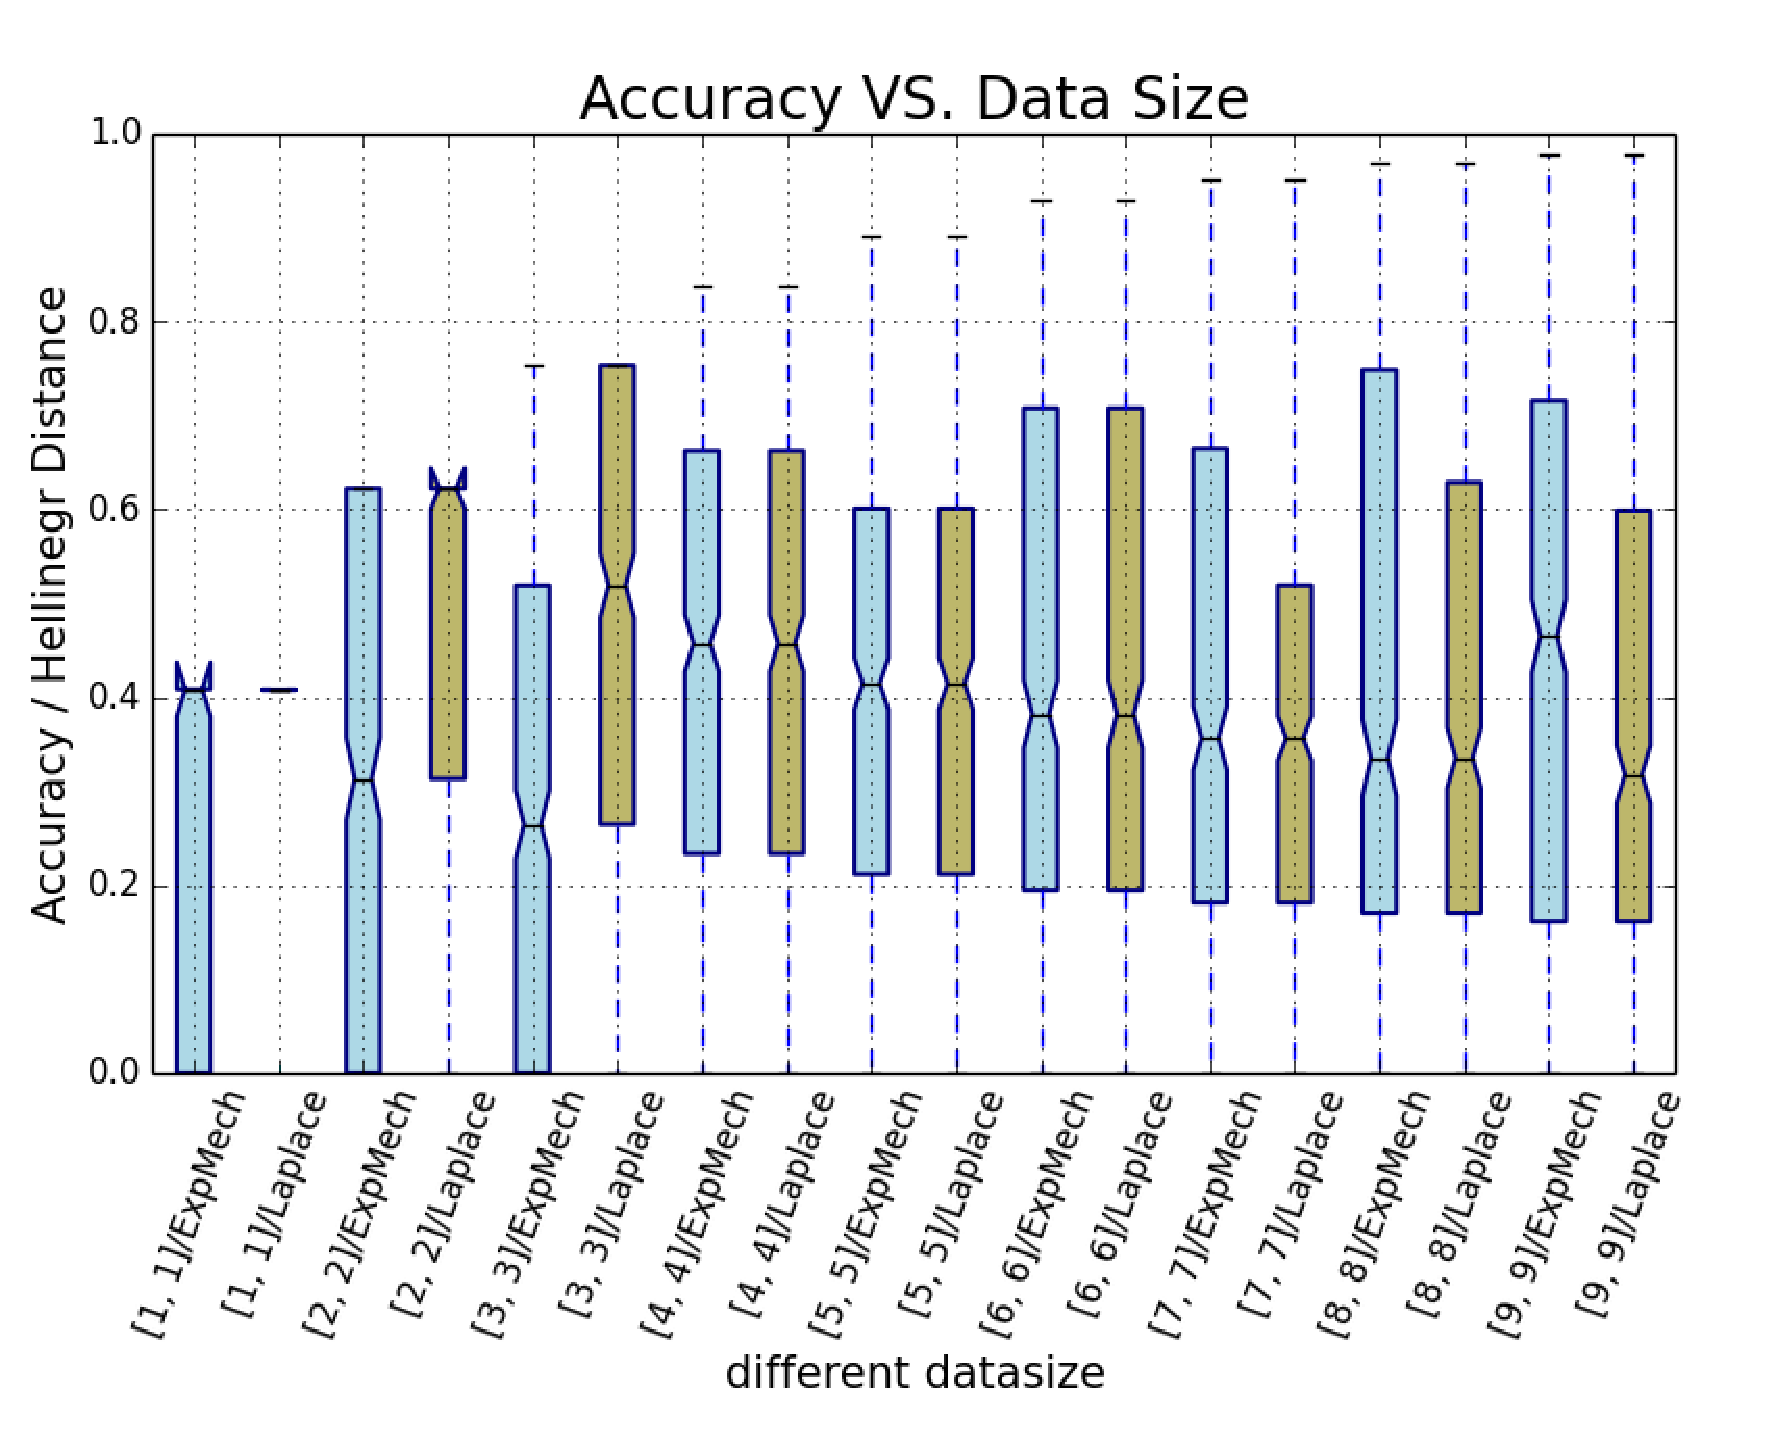
\includegraphics[width=0.3\textwidth]{accuracy_vs_datasize_1_1.eps}}
  \subfigure[three dimensions with $\dirichlet (1,1,1)$ prior distribution]{
    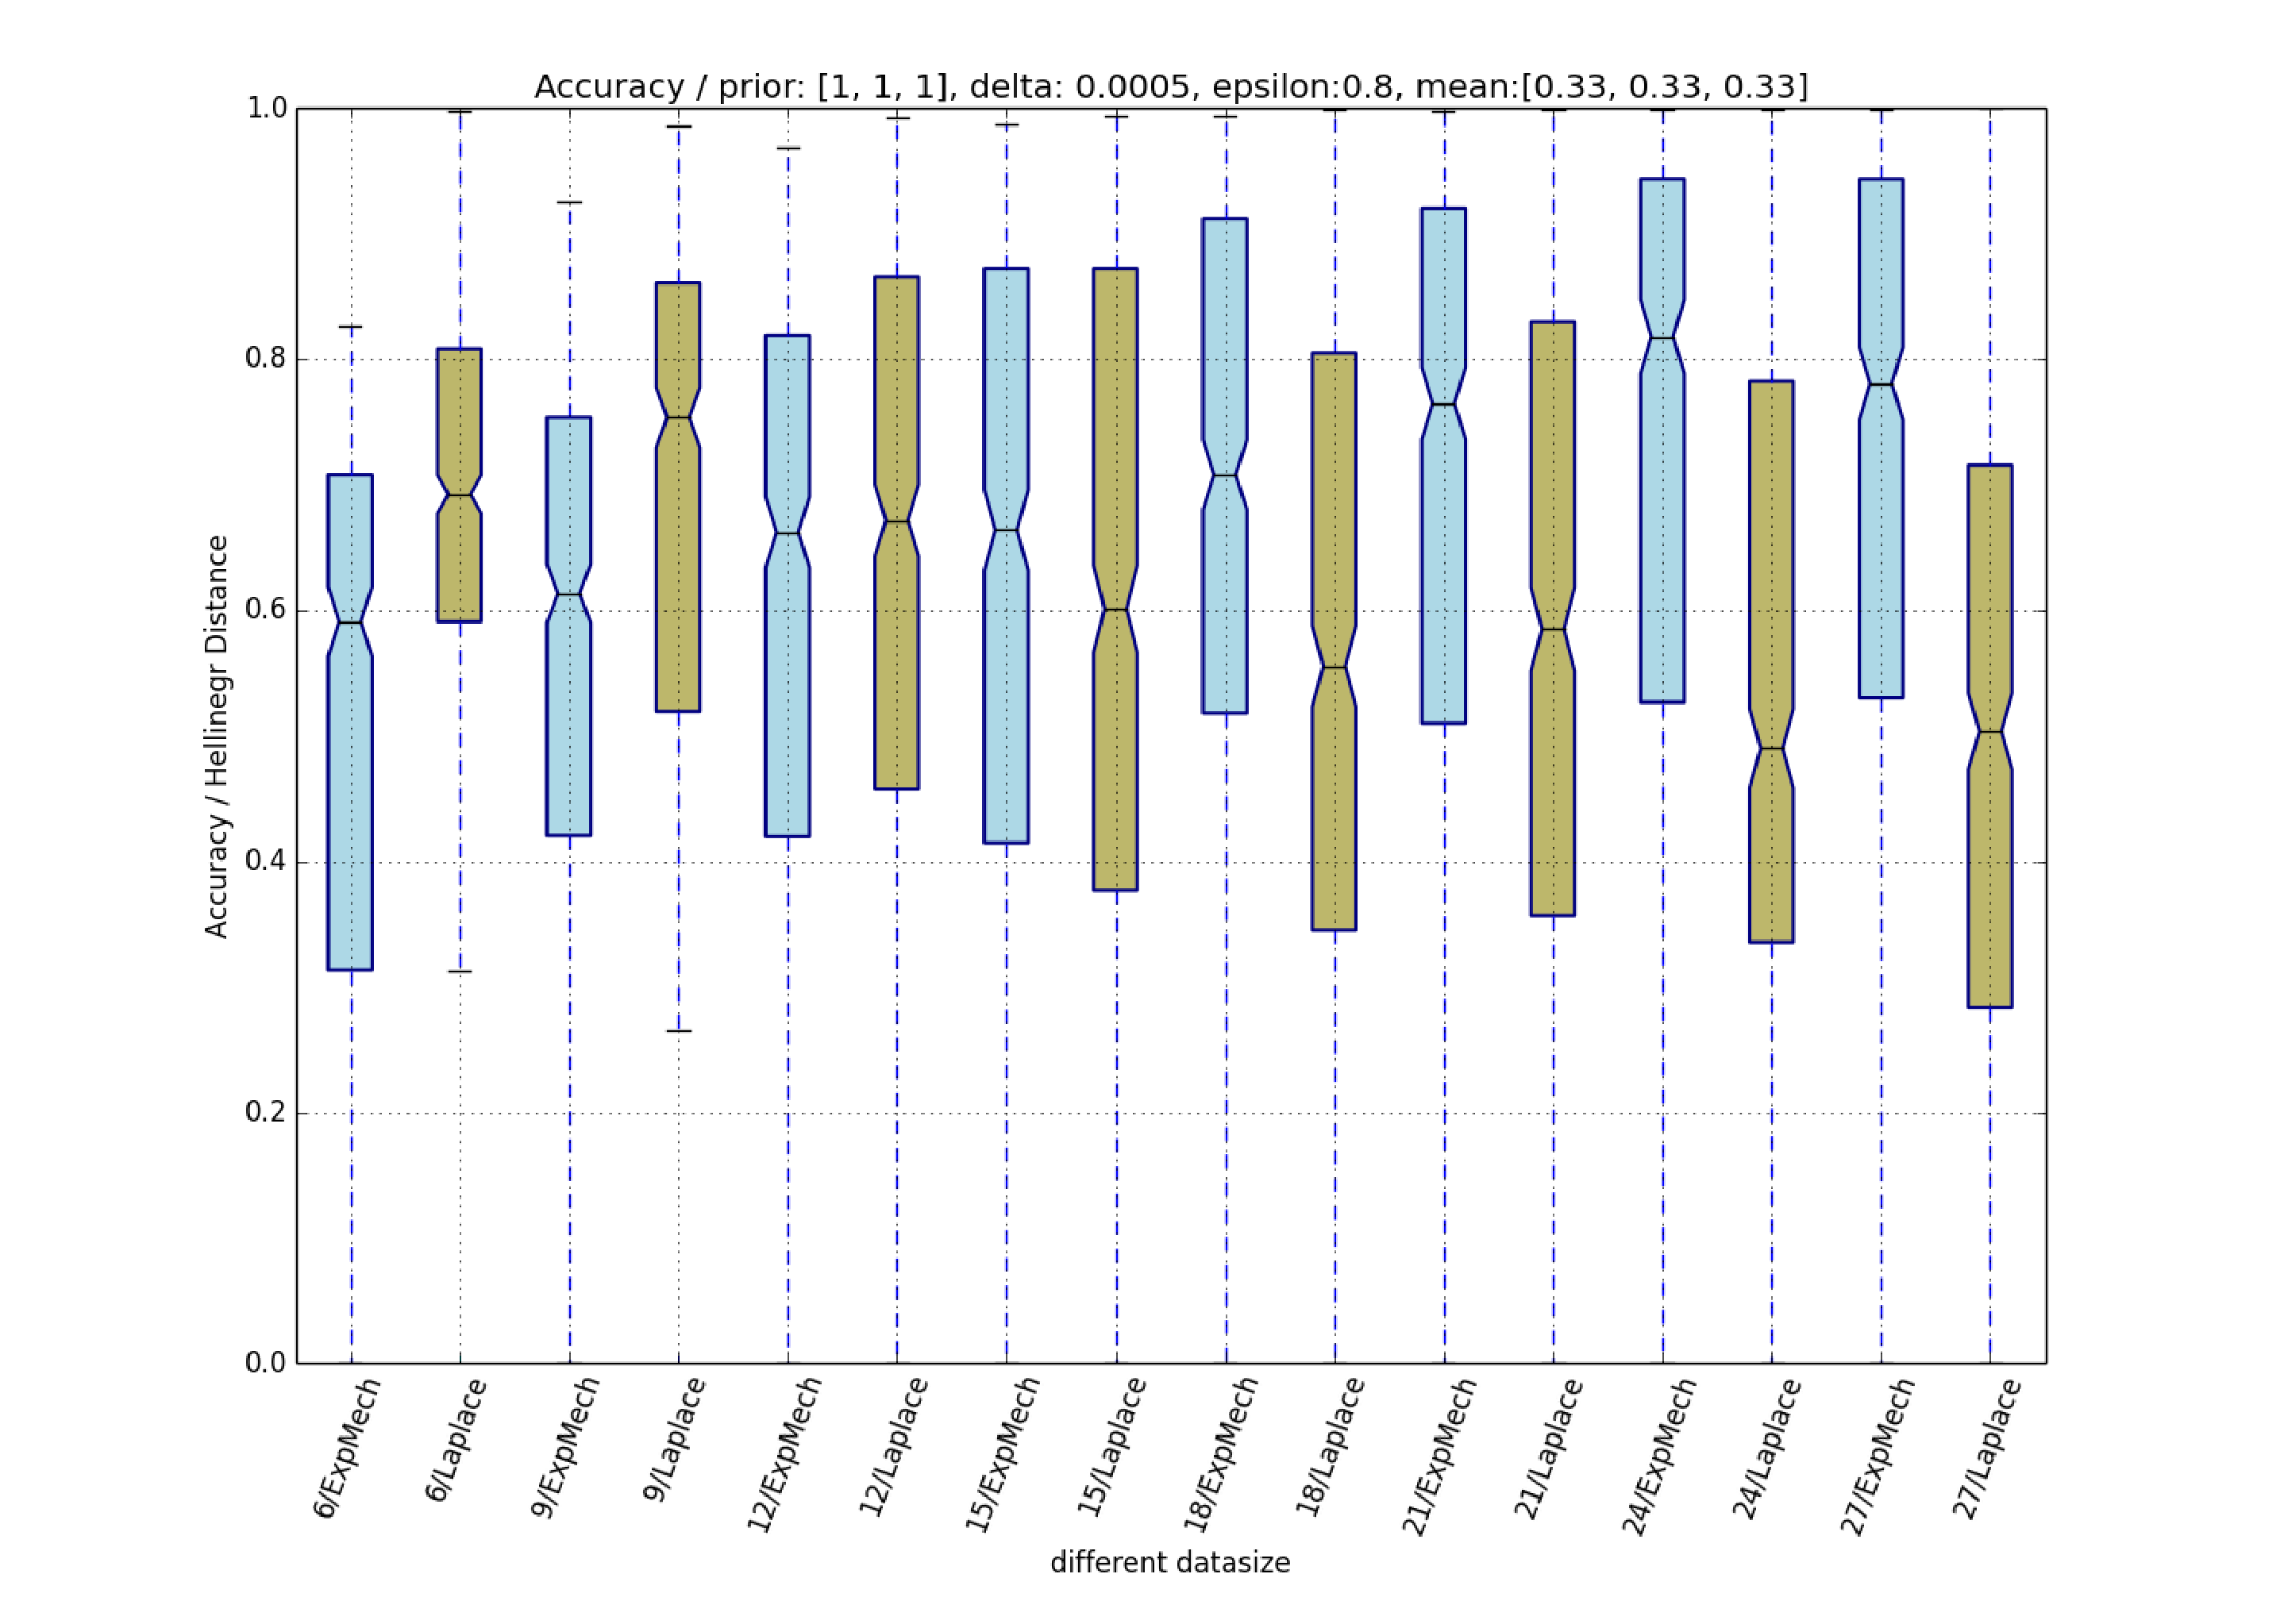
\includegraphics[width=0.3\textwidth]{accuracy_vs_datasize_1_1_1.eps}} 
\caption{Accuracy measurement based on Hellinger distance wrt. different datasizes. Settings: observed data are uniformly distributed, $\epsilon = 0.8$ and $\delta = 0.00000001$}
\label{fig_vs_datasize}
\end{center}
\end{figure}

In Fig. \ref{fig_vs_datasize}, both of the two plots show that when data size go larger, accuracy of our exponential mechanism are decreasing. In Fig. \ref{fig_vs_datasize}(a), when the data size is smaller than 12, we can beta Laplace mechanism but fail when data size larger than or equal to 12. Same as in Fig. \ref{fig_vs_datasize}(b), we can beat Laplace mechanism when data size is smaller than 15 and fail otherwise.

\subsubsection{Accuracy Evaluation wrt. Dimensions}
\label{subsubsec_vs_dimension}


\begin{figure}[ht]
\centering
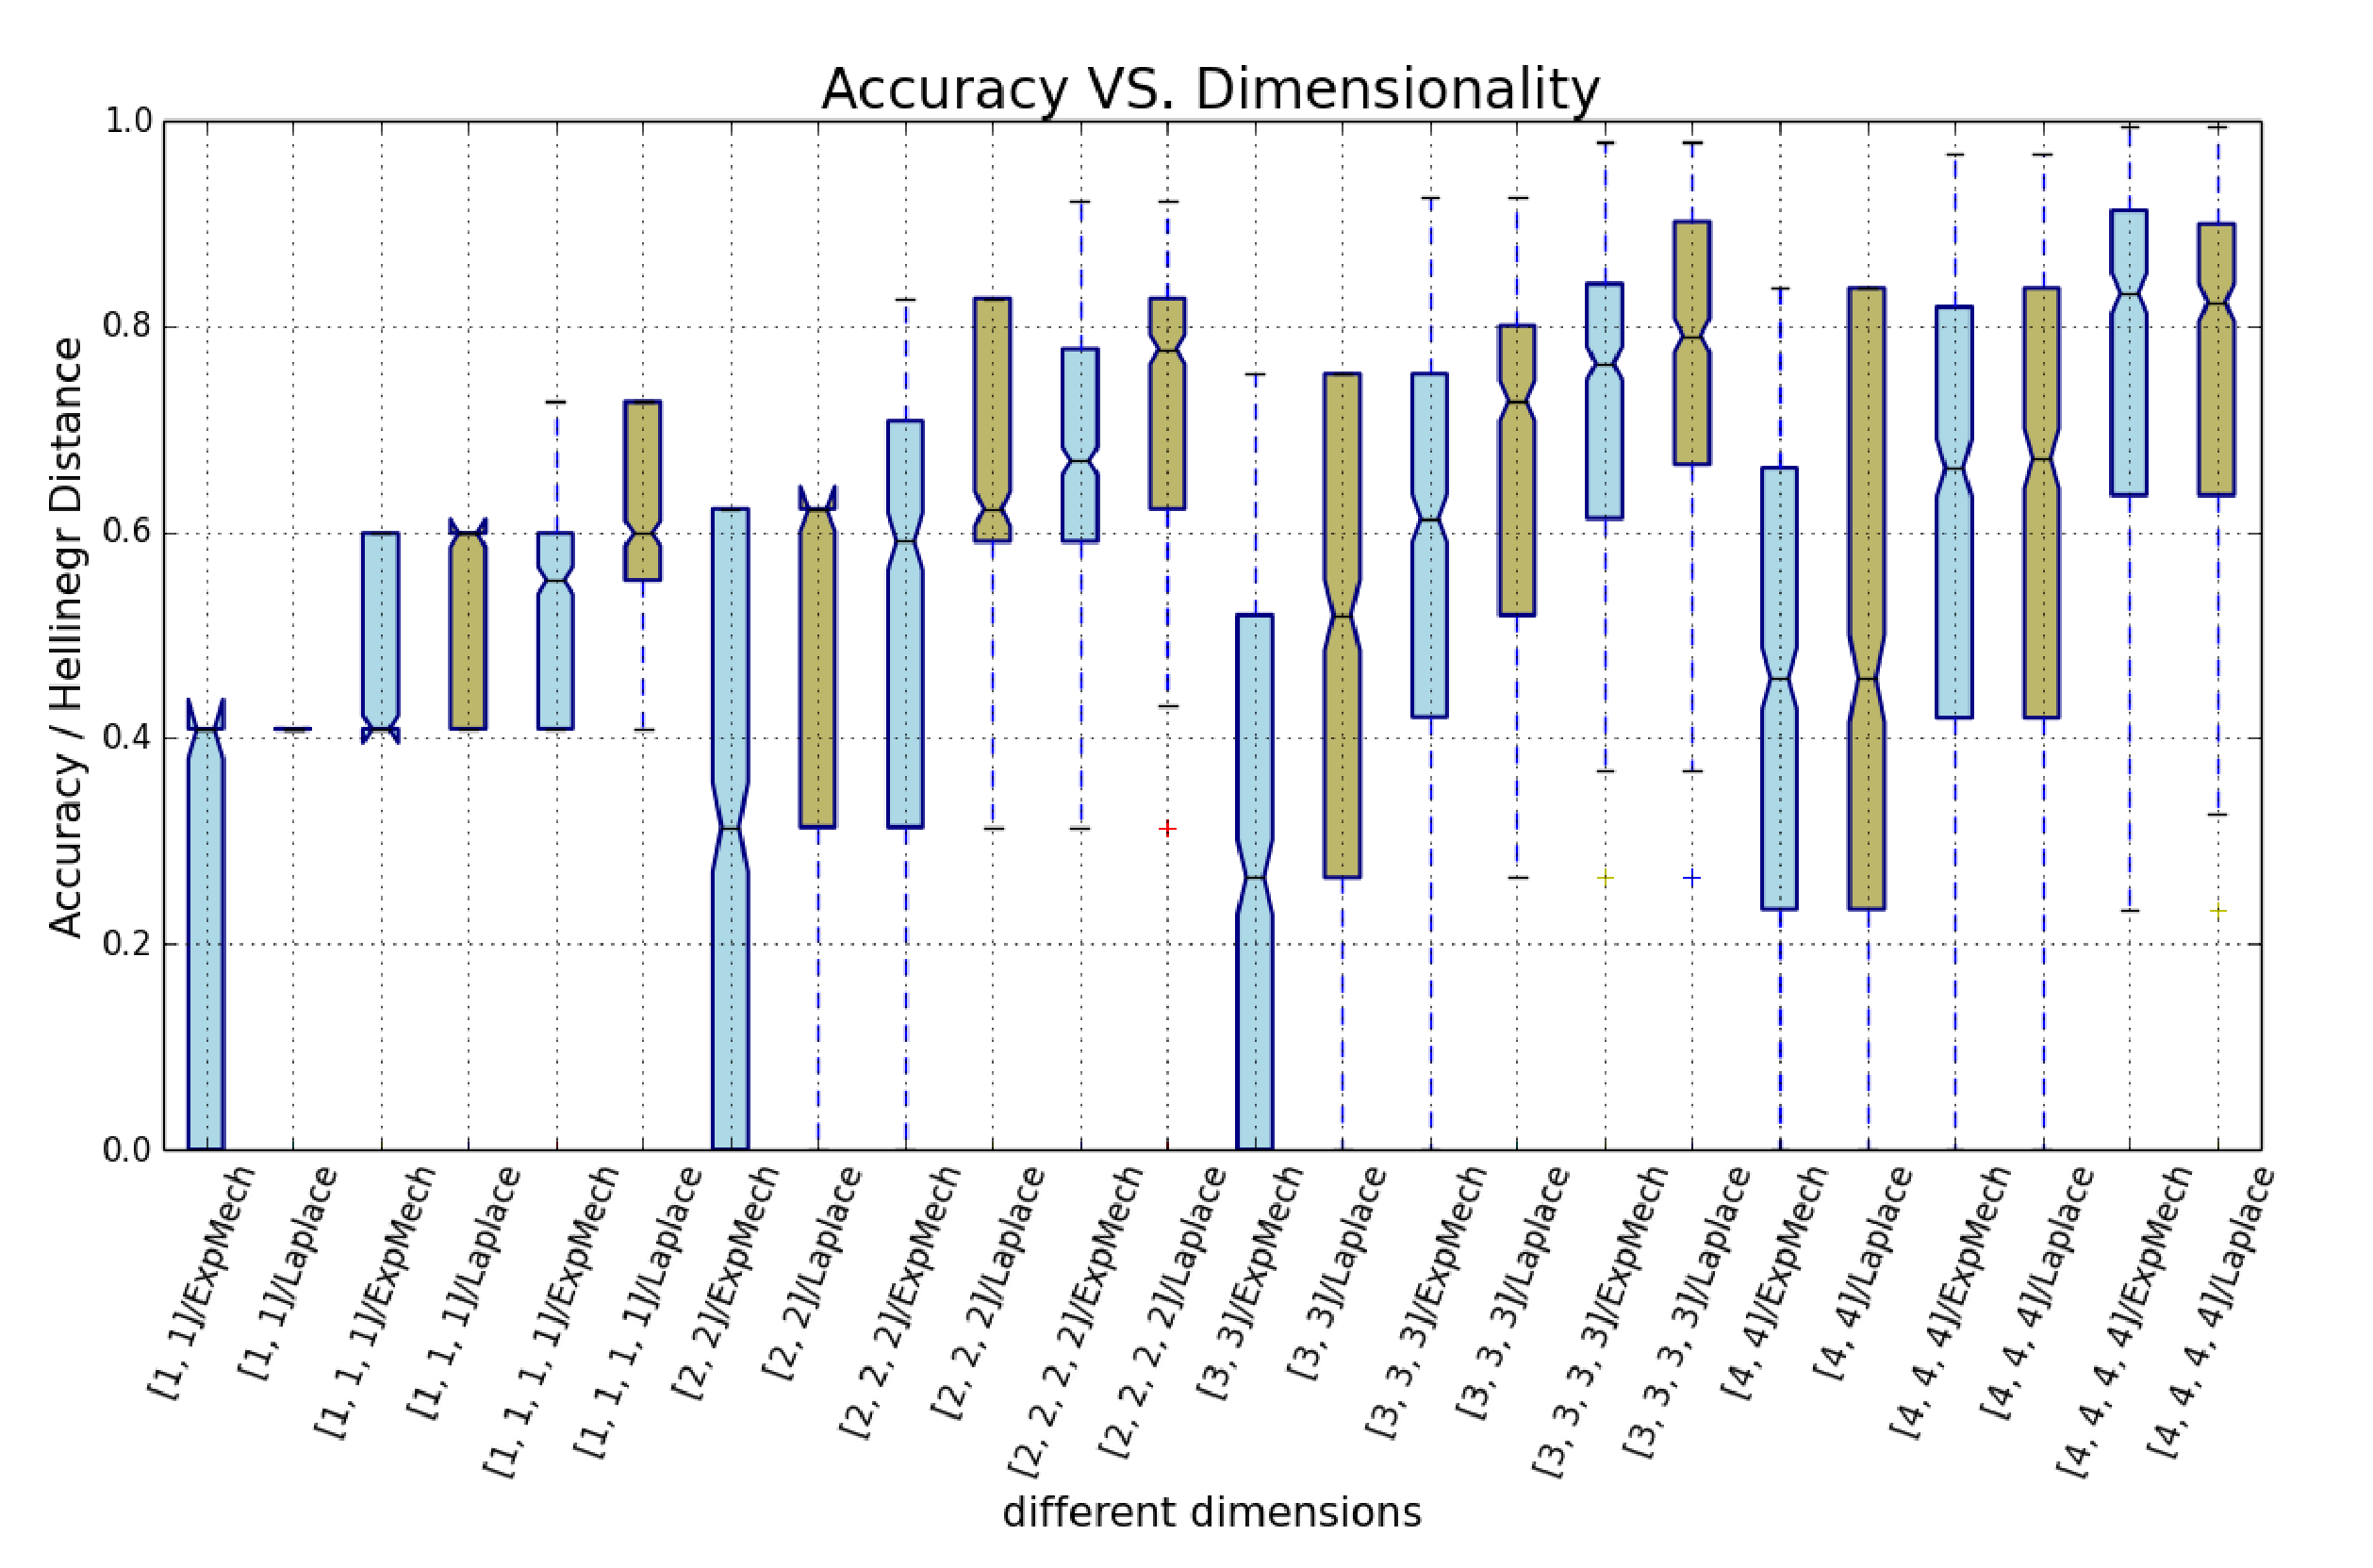
\includegraphics[width=0.45\textwidth]{accuracy_vs_dimension.eps}
\caption{Accuracy measurement based on Hellinger distance wrt. different dimensions and data size. Settings: observed data are uniformly distributed, $\epsilon = 0.8$ and $\delta = 0.00000001$, prior distributions are all $1$ in every dimension}
\label{fig_vs_dimension}
\end{figure}

In Fig. \ref{fig_vs_dimension}, x-axis are observed data sets of different size and dimensions. The plot shows that dimensions have similar influence on our exponential mechanism and the Laplace mechanism. Accuracy of two mechanisms both decrease when dimensions go larger. We will be beat by Laplace mechanism when data size increase but will not be affected when dimensions increase. In other words, dimension has little influence on whether we will beat Laplace mechanism.


\subsubsection{Accuracy Evaluation wrt. Data variance}
\label{subsubsec_vs_variance}

\begin{figure}[ht]
\centering
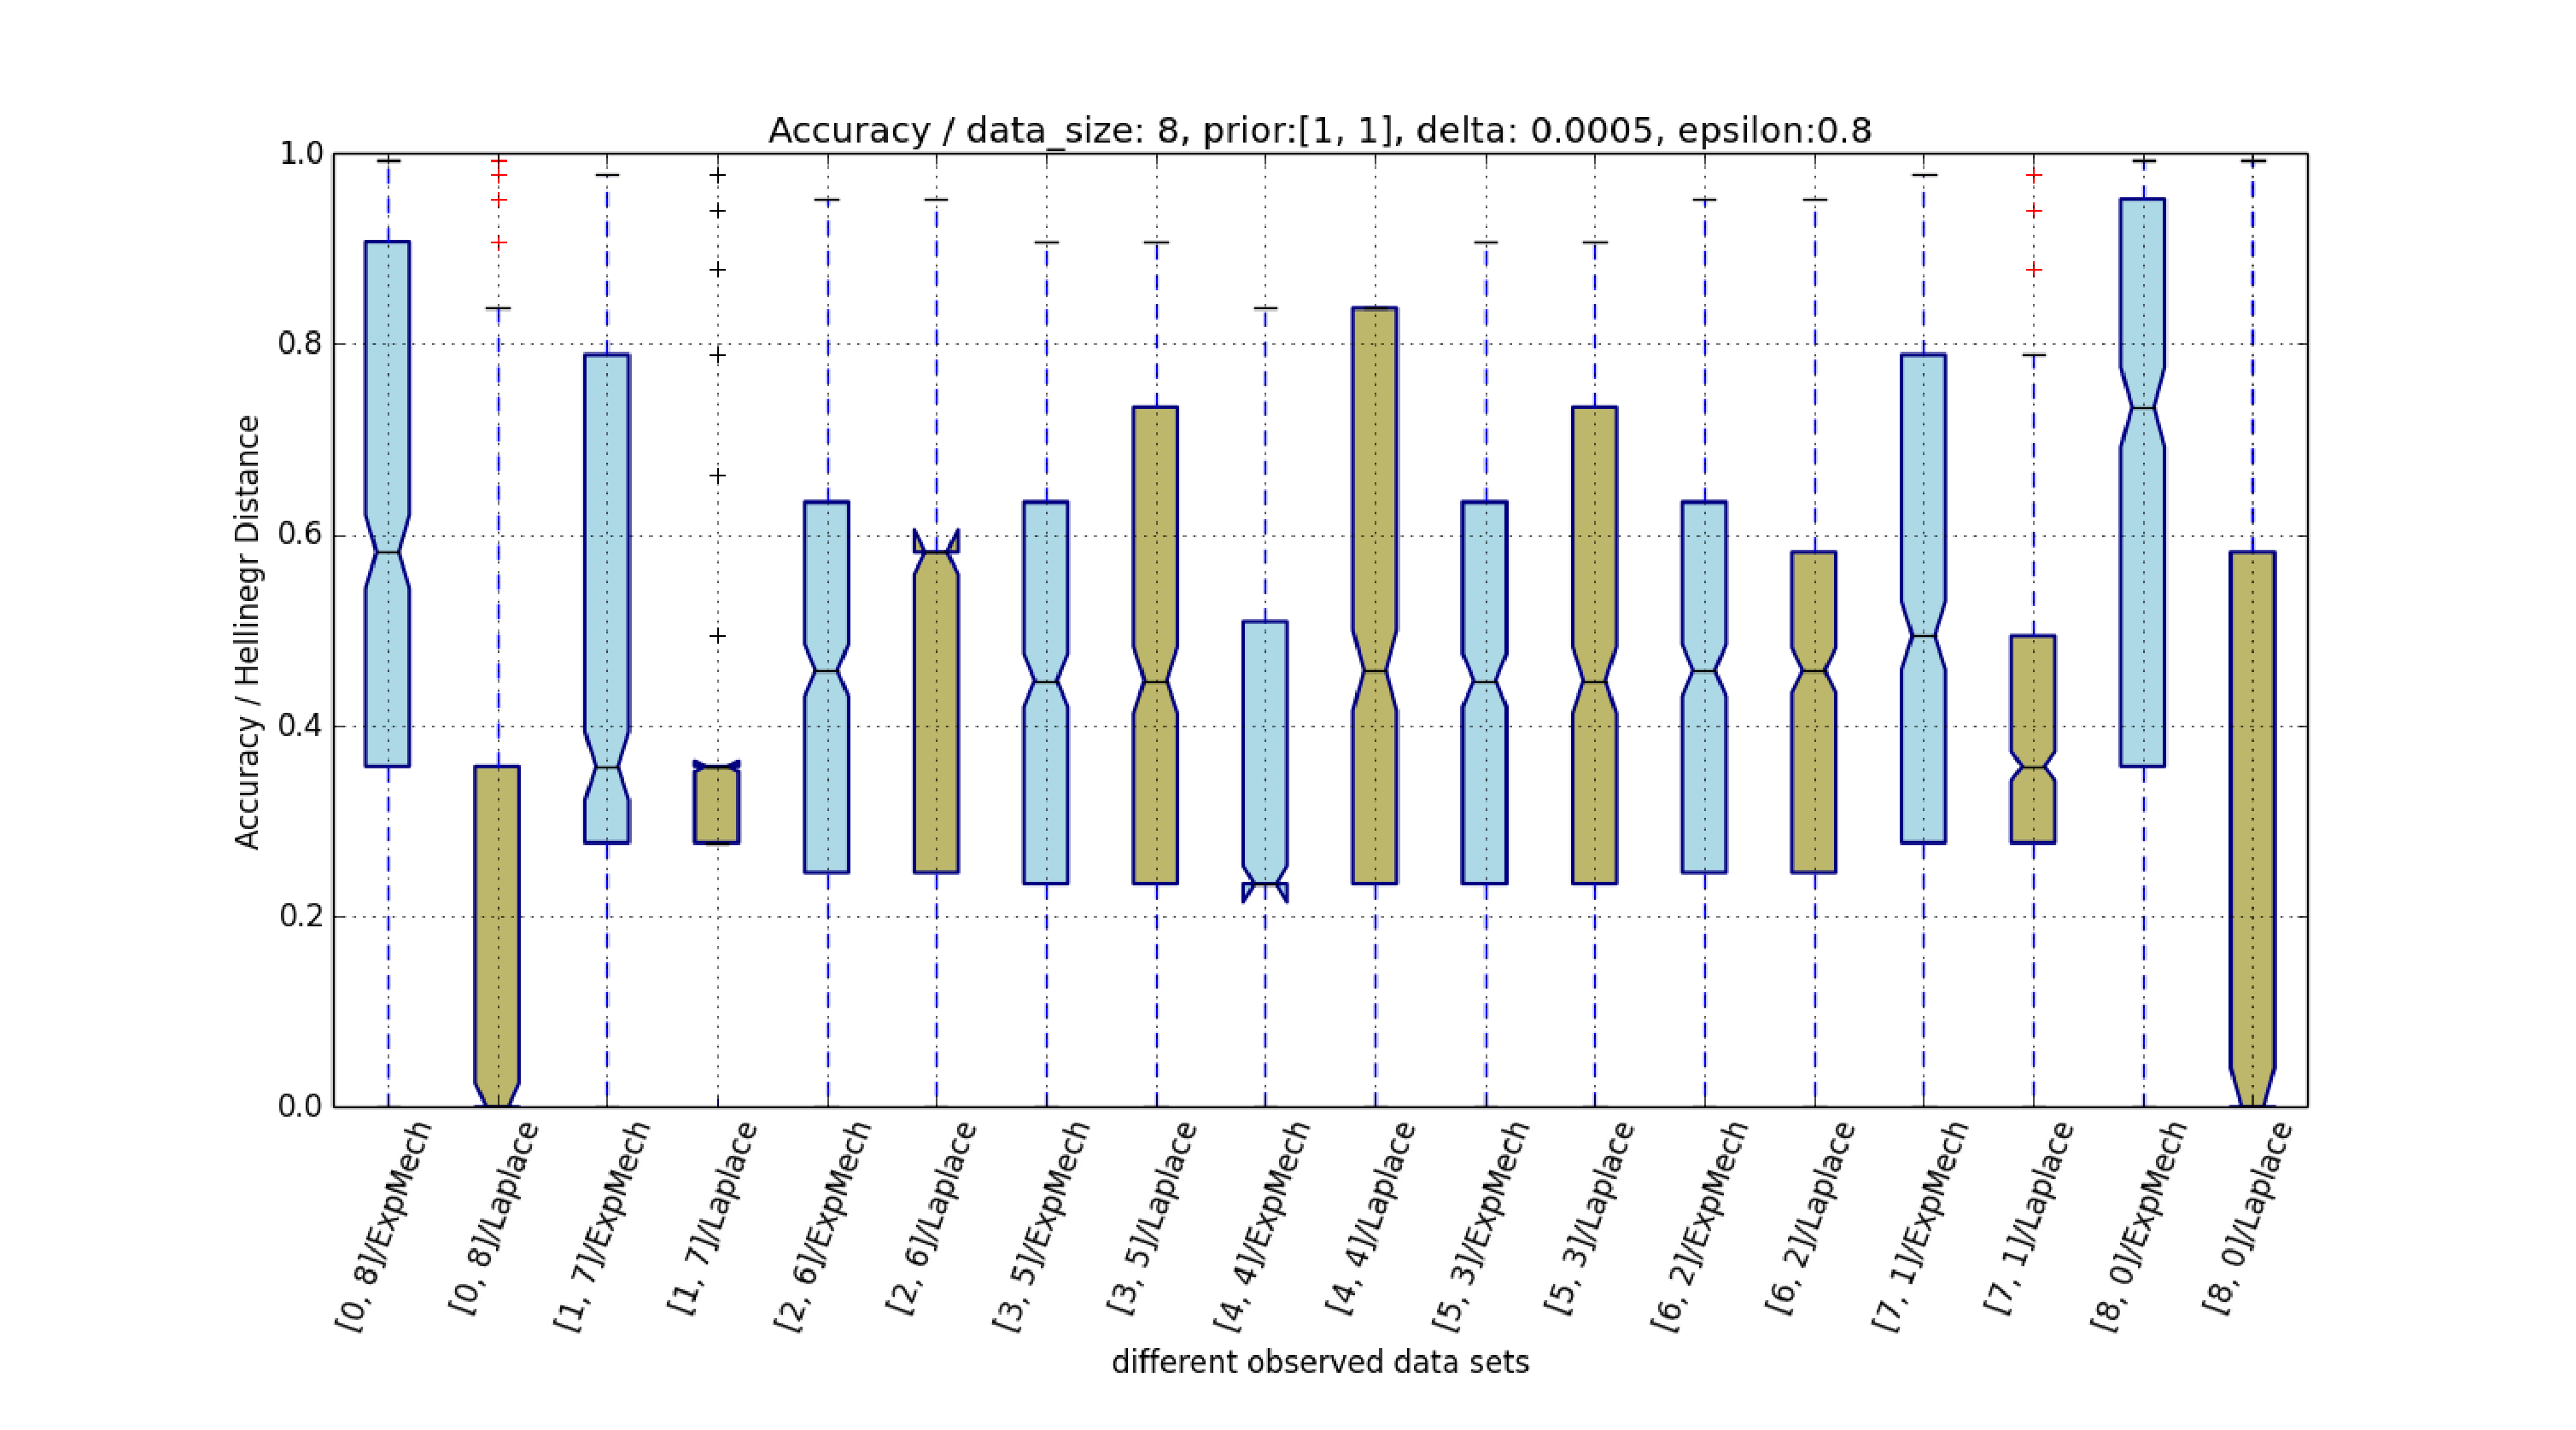
\includegraphics[width=0.45\textwidth]{accuracy_vs_mean_1_1.eps}
\caption{Accuracy measurement based on Hellinger distance wrt. different data variance. Settings: $\epsilon = 0.8$ and $\delta = 0.00000001$, prior distributions are all $1$ in every dimension}
\label{fig_vs_variance}
\end{figure}

In Fig. \ref{fig_vs_variance}, x-axis are observed data sets of different variances (or means). We study this variable under two-dimension $\betad$ distribution in order to be concise. It shows that our mechanism's accuracy is better when data variance go smaller, meanwhile Laplace mechanism go worse. We will beat Laplace mechanism when observed data are more uniformly.



\subsubsection{Accuracy Evaluation wrt. Prior Distribution}
\label{subsubsec_vs_prior}

\begin{figure}[ht]
\centering
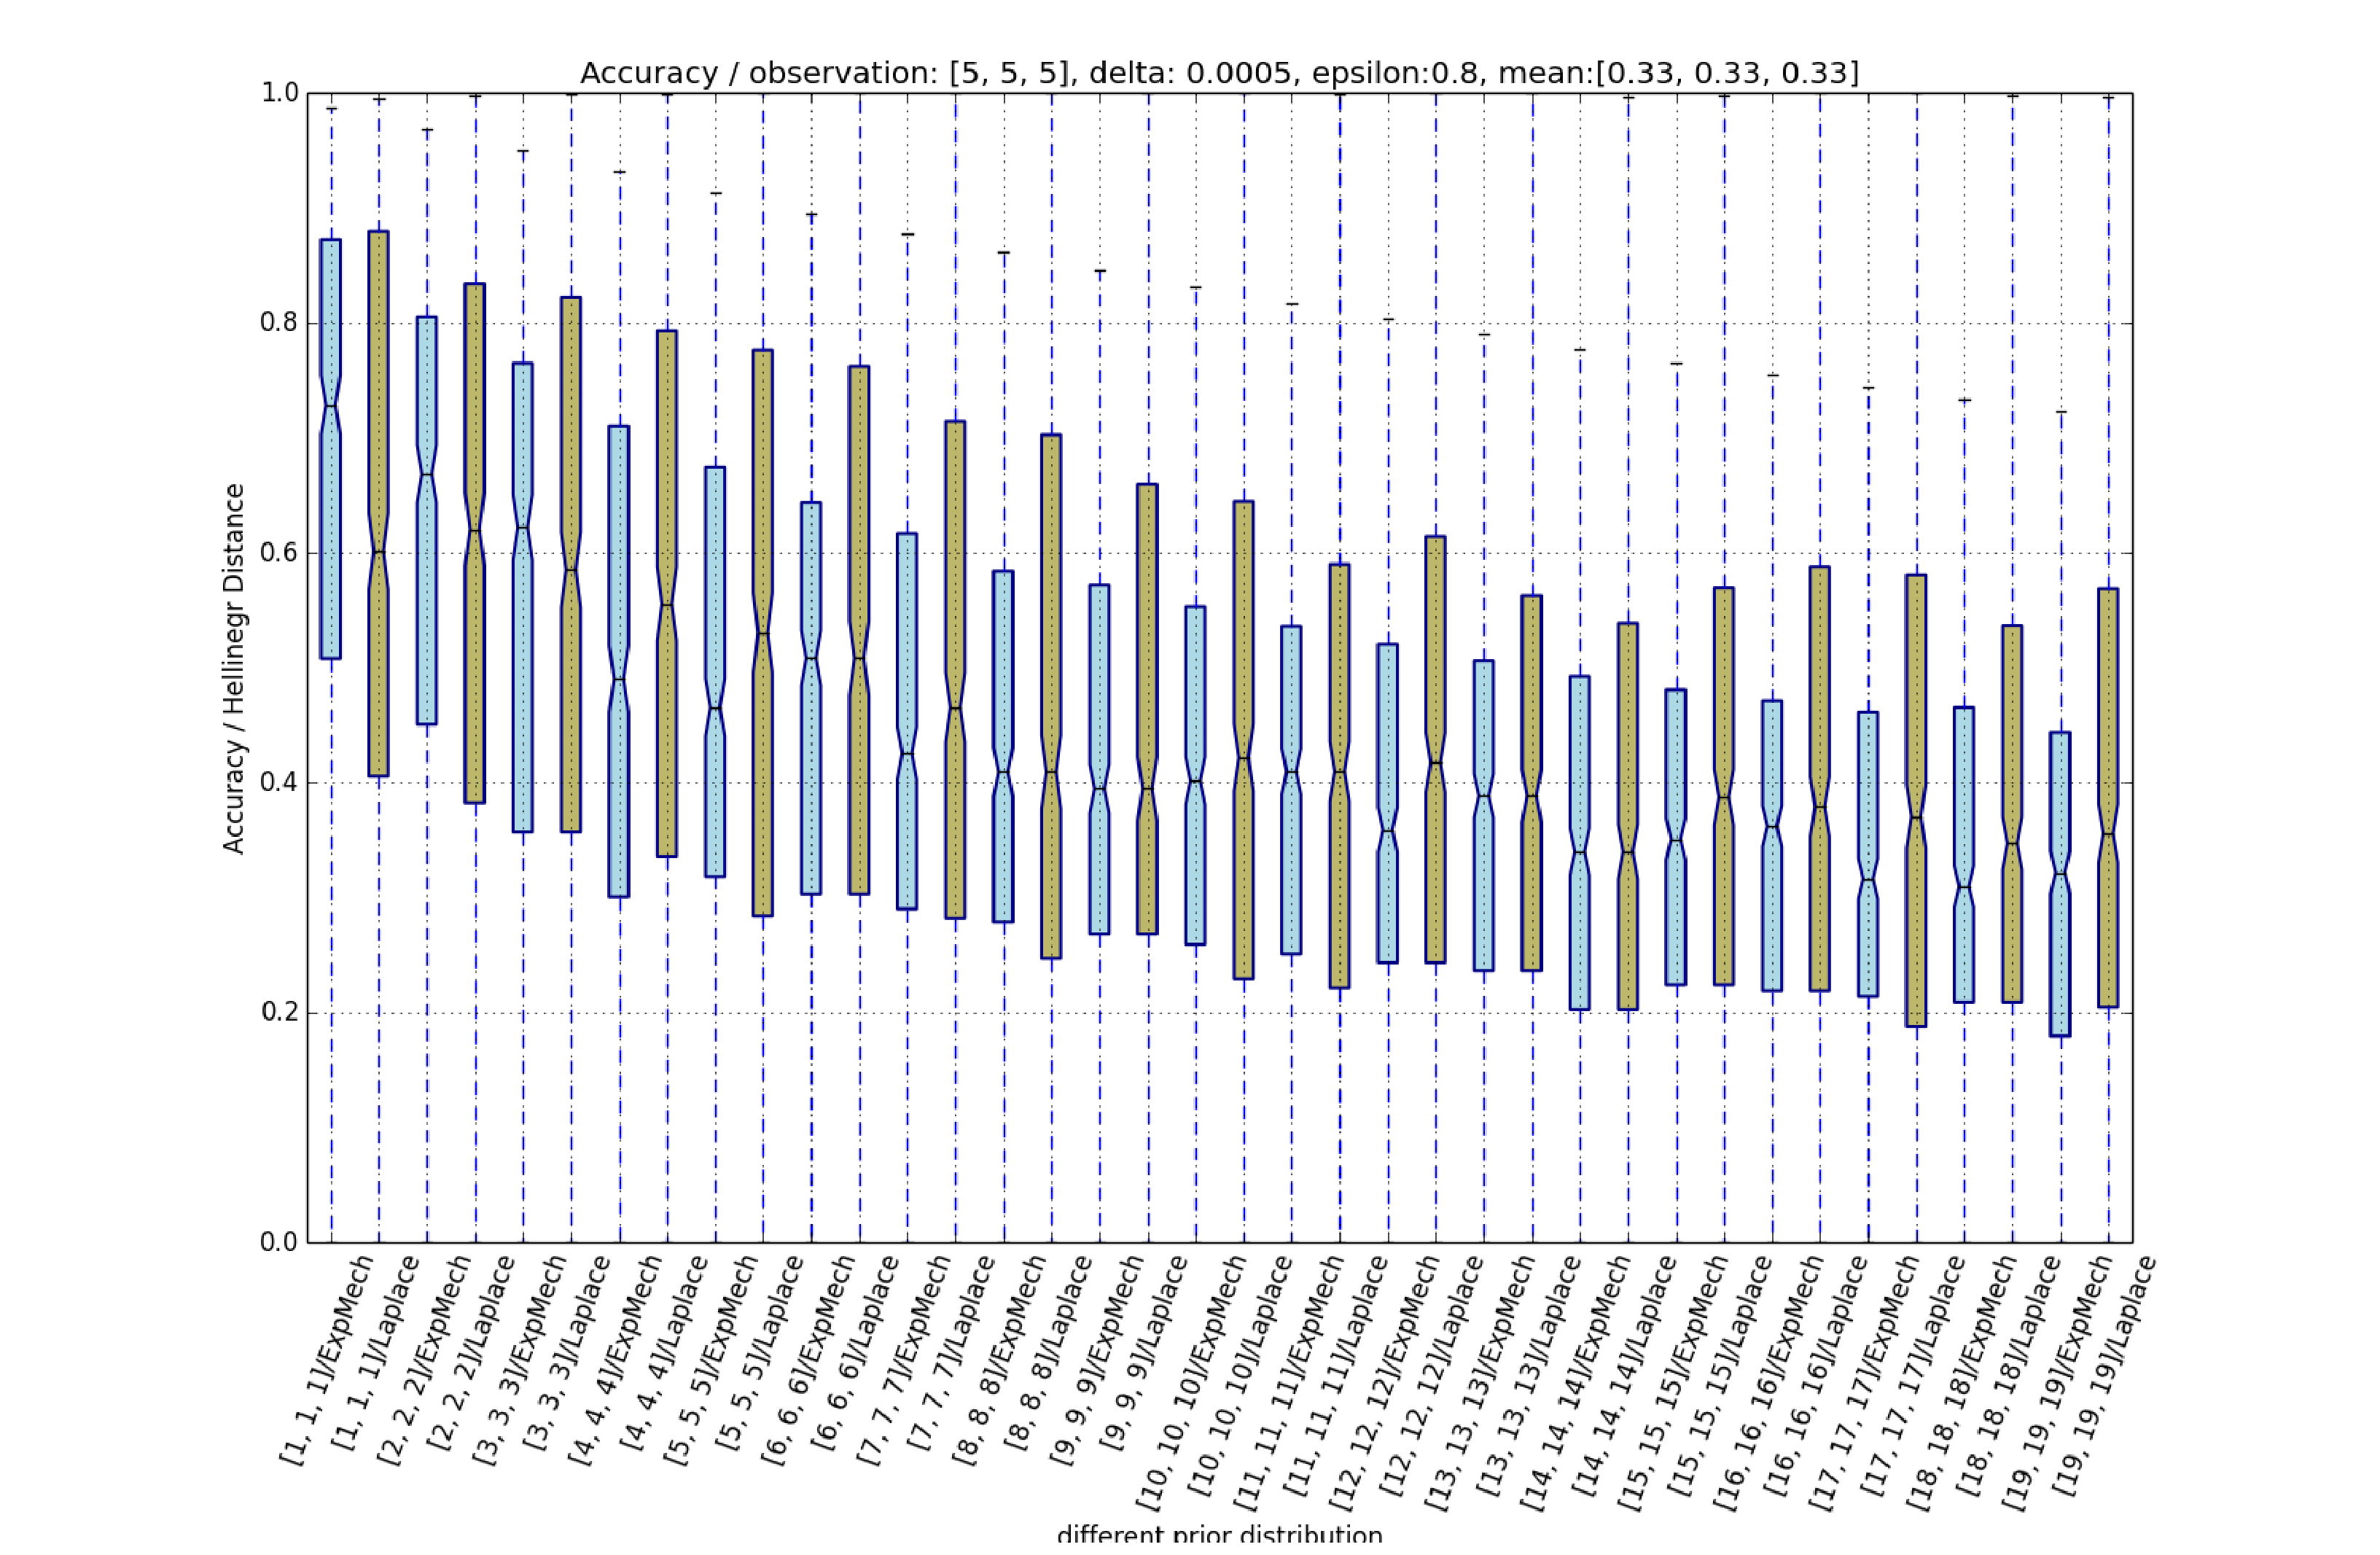
\includegraphics[width=0.45\textwidth]{accuracy_vs_prior_5_5_5.eps}
\caption{Accuracy measurement based on Hellinger distance wrt. different prior distribution. Settings: $\epsilon = 0.8$ and $\delta = 0.00000001$, observed data set is: $[5,5,5]$}
\label{fig_vs_prior}
\end{figure}

In Fig. \ref{fig_vs_prior}, we study this variable under setting that observed data set is $[5,5,5]$ because in Fig. \ref{fig_vs_datasize} Laplace mechanism beat us when data size is 15 and uniformly distributed. The plot shows that in the beginning we cannot beat Laplace but when prior distribution grow larger, we perform better and better and beat Laplace mechanism finally.



% \subsubsection{Accuracy Evaluation wrt. Prior Distribution and Data Variance}
% \label{subsubsec_vs_prior_variance}

% \begin{figure}[ht]
% \centering
% 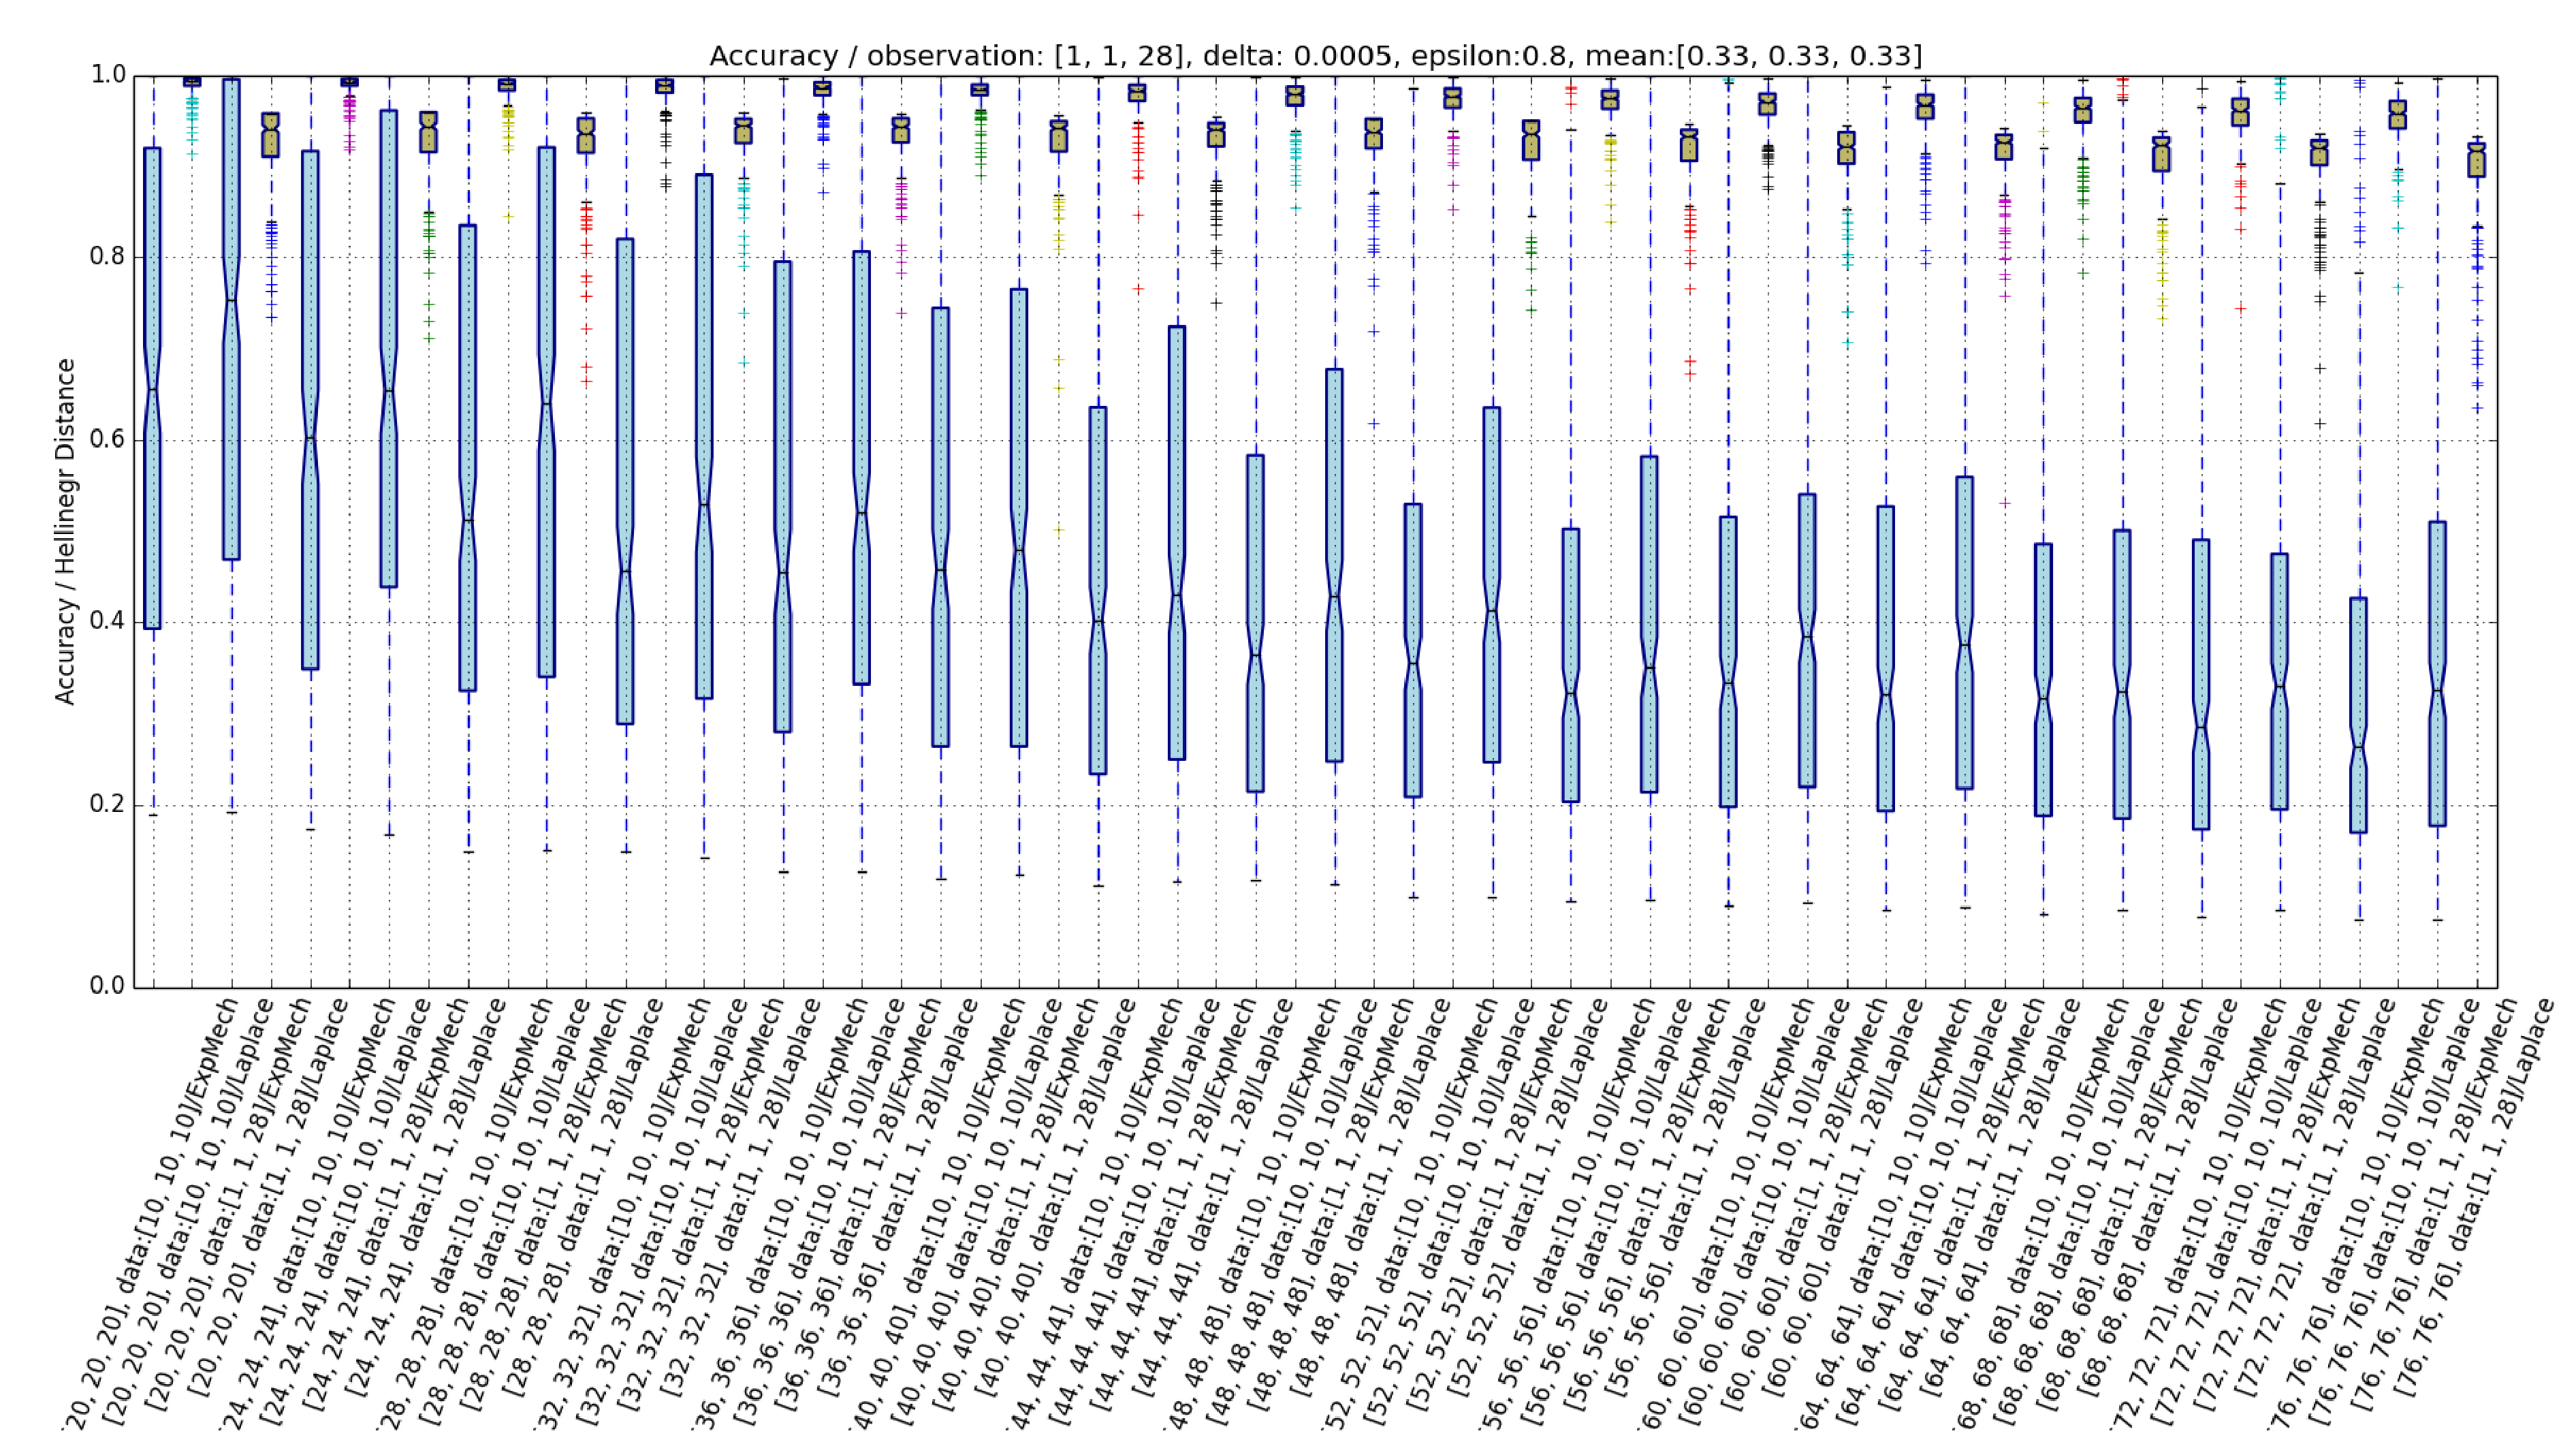
\includegraphics[width=0.45\textwidth]{Accuracy_VS_Prior_mean.eps}
% \caption{Accuracy measurement based on Hellinger distance wrt. different prior distribution and data variances. Settings: $\epsilon = 0.8$ and $\delta = 0.00000001$, observed data sets are $[10,10,10]$ and $[1,1,28]$ and prior distributions are range from $[20,20,20]$ to $[76,76,76]$}
% \label{fig_vs_prior_variance}
% \end{figure}

% Here, we change the prior distribution and data variance in the same time. As shown in Fig. \ref{fig_vs_prior_variance}, our exponential mechanism do better in uniform data set than in edging data set while Laplace mechanism on the contrary. Moreover, our mechanism is improving continuously and significantly as prior distribution increasing while Laplace mechanism isn't.


\section{Conclusions}
We can obtain some preliminary conclusions: 
\begin{enumerate}
	\item We can beat Laplace mechanism when data size is small.
	\item We will beat Laplace mechanism when observed data are more uniformly.
  \item When prior distribution grow larger, we perform better and better and beat Laplace mechanism finally.
\end{enumerate} 

In consequence, we have a better accuracy in small data size, in larger prior and in uniformly data.



\bibliographystyle{ACM-Reference-Format}
\bibliography{bayesian.bib}

\end{document}
 % TODO: replace with your brilliant paper!
% 
%packages
\usepackage{natbib}
\usepackage{amsmath}
\usepackage{amsthm}
\usepackage{mathtools}
\usepackage{mdframed}
\usepackage{subfigure}
\usepackage{booktabs}
% \usepackage{hyperref}
\usepackage{subfigure}
\usepackage{siunitx} % Provides the \SI{}{} and \si{} command for typesetting SI units
\usepackage{graphicx} % Required for the inclusion of images
% \usepackage{natbib} % Required to change bibliography style to APA
\usepackage{datetime}
\usepackage{lscape}
\usepackage{algorithm}
\usepackage{algorithmic}
\usepackage{xspace}
\usepackage[english]{babel} % English language/hyphenation
\usepackage{proof}
\usepackage{booktabs} % Top and bottom rules for tables
\usepackage[colorlinks, allcolors = blue,]{hyperref}
\usepackage{accents}
\usepackage{amsfonts}
\usepackage{stmaryrd}
\usepackage{amsmath,amsthm,amssymb,latexsym} 
\usepackage{microtype}
\usepackage{graphicx}
\usepackage{subfigure}
\usepackage{booktabs} % for professional tables
\usepackage{hyperref}
\usepackage{icml2019}
\usepackage{lipsum}

\usepackage{authblk}


%new commands
\newcommand{\theHalgorithm}{\arabic{algorithm}}
\newtheorem{definition}{Definition}
\usepackage{cancel}
\usepackage[normalem]{ulem}
\newcommand{\dataobs}{\textbf{x}}
\newcommand{\adj}[2]{\textbf{adj}(#1,#2)}
\newcommand{\candidateset}{\mathcal{R}_{\textup{post}}}
\newcommand{\bprior}{\boldsymbol{\beta}_{\textup{prior}}}
\newcommand{\bysinfer}{\mathsf{Infer}}
\newcommand{\betad}{\mathsf{Beta}}
\newcommand{\betaf}{\textup{B}}
\newcommand{\mbetaf}{\boldsymbol{\textup{B}}}
\newcommand{\vtheta}{\boldsymbol{\theta}}
\newcommand{\valpha}{\boldsymbol{\alpha}}
\newcommand{\vbeta}{\boldsymbol{\beta}}
\newcommand{\lapmech}{\mathsf{LSDim}}
\newcommand{\ilapmech}{\mathsf{LSHist}}
\newcommand{\binomial}[2]{\mathsf{Bin}(#1, #2)}
\newcommand{\multinomial}[2]{\mathsf{Mult}(#1, #2)}
\newcommand{\expmech}{\mathsf{EHD}}
\newcommand{\hexpmech}{\mathsf{EHDS}}
\newcommand{\lexpmech}{\mathsf{EHDL}}
\newcommand{\hexpmechd}{\mathsf{expMech}^{D}_{\hellinger}}
\newcommand{\privinfer}{\mathsf{PrivInfer}}
\newcommand{\hlg}{\mathsf{H}}
\newcommand{\dirichlet}[1]{\mathsf{Dir}(#1)}
\newcommand{\alphas}{\boldsymbol{\alpha}}
\newcommand{\xis}{\boldsymbol{\xi}}
\newcommand{\iverson}[1]{[#1]}
\newcommand{\datauni}{\mathcal{X}}
\newcommand{\hellinger}{\mathcal{H}}
\newcommand{\ux}[1]{u(\textbf{x}, {#1})}
\newcommand{\uxadj}[1]{u(\textbf{x}', {#1})}
\newcommand{\cardinality}[2]{\mathcal{C}^{#1}_{#2}}
\newcommand{\range}{\mathcal{O}}
\newcommand{\nomalizer}[1]{\sum\limits_{r'\in \mathcal{R}_{\textup{post}}} \exp \big(\frac{-\epsilon\cdot \mathcal{H} (\mathsf{BI}(#1),r')}{4 \cdot S(#1)}\big)}

\newcommand{\unomalizer}[1]{\sum\limits_{r'\in \mathcal{R}_{\textup{post}}} \exp \big(\frac{-\epsilon\cdot u(#1, r')}{4 \cdot S(#1)}\big)}


\newcommand{\hexpmechPr}[2]{\underset{z \thicksim \hexpmech(#1)}{\Pr}\left[ #2 \right]}
\newcommand{\lapmechPr}[2]{\underset{z \thicksim \lapmech(#1)}{\Pr}\left[ #2 \right]}

\newcommand{\ilapmechPr}[2]{\underset{
{z \thicksim \ilapmech(#1)}
}{\Pr}\left[ #2 \right]}

\newtheorem{thm}{Theorem}[section]

\newtheorem{lem}{Lemma}[section]

\newtheorem{assert}{Assertion}[lem]
\newcommand{\lap}[2]{\mathsf{Lap}(#1, #2)}
\newcommand{\todo}[1]{{\footnotesize \color{red}\textbf{[[ #1 ]]}}}

\section{Bayesian Inference Background}
Given a prior belief $\Pr(\theta)$ on some parameter $\theta$,
and given an observation $\dataobs$,
the posterior distribution on $\theta$ given $\dataobs$ is computed as:
\[
  \Pr(\theta | \dataobs) = \frac{Pr(\dataobs | \theta) \cdot \Pr(\xis)}{\Pr(\dataobs)}
\]
where the expression  $\Pr(\dataobs | \theta)$ denotes the \emph{likelihood} of $\theta$ when
\dataobs~ is observed. Since we consider \dataobs to be fixed the likelihood is a function of $\theta$.
For the same reason $\Pr(\dataobs)$ is a constant independent of $\theta$.
Usually in statistics the prior distribution $\Pr(\theta)$ is chosen so that it represents
the initial belief on $\theta$. That is, when no data has been observed. In practice though,
prior distributions and likelihood functions are usually chosen so that the posterior
belongs to the same \emph{family} of distributions. In this case we say that the prior
is conjugate of the likelihood function. Using conjugate priors simplify calculcations and allows
for inference to be performed in a recursive fashion over the data.
In this work we will consider a specific instance of Bayesian inference and one of its generalizations.
Specifically, we will consider the situation where $\theta$ represents the parameter --informally called \emph{bias})--
of a Bernoulli distributed random variable, and its immediate generalization where the parameter $\vtheta$ represents
the the vector of parameters of a categorical distributed random variable.
In the former case the prior distribution over $\theta\in [0,1]$ is going to be a beta distribution, $\betad(\alpha, \beta)$, with parameters
$\alpha,\beta\in\mathbb{R}^{+}$, and with p.d.f:
\[
  \Pr(\theta)\equiv \frac{\theta^{\alpha} (1- \theta)^{\beta}}{\betaf(\alpha,\beta)}
\]
where $\betaf(\cdot,\cdot)$ is the beta function.
The data $\dataobs$ will be a sequence of $n\in\mathbb{N}$ 0/1 values, that is $\dataobs=\ll x_1,\dots x_n \gg, x_i\in\{0,1\}$, and the likelihood function is:
\[
  \Pr(\dataobs | \theta)\equiv \theta^{a}(1-\theta)^{n-a}
\]
where $a=\displaystyle\sum_{i=1}^{n}\mathrm{x_i}$.
From this it can easily be derived that the posterior distribution is:
\[
  \Pr(\theta|\dataobs)=\betad(\alpha+a,\beta+n-a)
\]
In the latter case the prior distribution over $\vtheta\in [0,1]^{k}$ is given by a Dirichelet distribution, $\dirichlet(\vtheta)$, for $k\in\mathbf{N}$,
and $\valpha\in(\mathbf{R^{+}})^{k}$, with p.d.f:
\[
  \Pr(\vtheta)\equiv\frac{1}{\mbetaf(\valpha)}\cdot \displaystyle\prod_{i=1}^{k}{\theta_i^{\alpha_i-1}}
\]
where $\mbetaf(\cdot)$ is the generealised beta function.
The data $\dataobs$ will be a sequence of $n\in\mathbb{N}$ values coming from a universe $\datauni$, such that $\mid\datauni \mid=k$.
The likelihood function will be:
\[
  \Pr(\dataobs|\vtheta)\equiv \displaystyle\prod_{a\in\datauni}\alpha_{a}^{z_a}
\todo{to check}\]
where $z_a=\displaystyle\sum_{i=1}^{n}\iverson{x_i=a}$, where in $\iverson{\cdot}$ we use
Iverson bracket notation. The posterior distribution over $\vtheta$ turns out to be
\[
  \Pr(\vtheta|\dataobs)=\todo{to type down}\dirichlet(\vtheta+...)
\]
\section{Problem Statement}
% When we try
% to make this distribution public, sensitive information of the data
% based on which the posterior drew from can be compromised. So, it is
% important to protect this posterior distribution. When our protection
% objective is a distribution rather than a numeric value or vector, it
% would be better to measure the accuracy by distance over
% distributions, for instance, Hellinger distance, than by numeric
% metrics like $\ell_1$-norm.
This work will show that the same mechanism can
perform differently when its accuracy is computed w.r.t to a metric
over probability measures (e.g total variation distance, or Hellinger distance)
from when the metric (e.g. $\ell_1$-norm) is over the parameters.  
\section{Technical Problem Statement}
\label{sec_bayesInfer}
The posterior belief about parameters $\xis$ is inferred from the
group of sensitive data. Because it is usually published in form of a
distribution, for example, $\betad(\alpha',\beta'), \cdots,$ itself
can relieve a lot of information about sensitive data. So, the
sensitive information we want to protect here is the posterior belief,
i.e., $Pr(\xis | \dataobs)$, rather than just a sample drew from
it\cite{foulds2016theory}. Then it will be better if we can use a
distance over two distributions to measure the accuracy than a
distance over just parameters or values when we are protecting a
distribution, for instance, Hellinger distance in our paper. When we
measure the accuracy between true posterior and protected posterior
using Hellinger distance, it would be better we can have a protection
mechanism based on Hellinger distance. However, current mechanisms are
mainly based on $l_1$ norm by Laplace mechanism
\cite{zhang2016differential} \cite{xiao2012bayesian}. That's why we
design our exponential mechanism over Hellinger distance to protect
the whole posterior distribution.


\section{Baseline Approach - Laplace Mechanism}
\label{sec_lap}
Based on the posterior results from Bayesian inference, we calculate the Laplace mechanism updates on posterior and get the private results under Laplace mechanism. In the case of $m$ dimension Dirichlet distribution, we will add $(m-1)$ i.i.d. Laplace noises $\{| Lap_1 |, | Lap_2 |, \cdots, | Lap_{m-1} |\}$ to the output, where $Lap_i = floor(Y)$, $Y \sim Lap(\frac{2}{\epsilon})$. The private posterior then will be $\dirichlet(\alpha_1 + n_1 + | Lap_1 |, \alpha_2 + n_2 + | Lap_2 |, \cdots, \alpha_m + n - (Lap_1 + \cdots + Lap_{m-1}))$.

\section{Our Approach - Exponential Mechanism with Smooth Sensitivity}
\label{sec_smoo}

% \subsection{Algorithm Setting up}
We define a new mechanism $\hexpmech(x)$ which is similar to the exponential mechanism where we use $\mathcal{R}$ as the set $\betaset$ of beta distributions with integer parameters summing up to $n+2$, as scoring function we use the Hellinger distance from $\bysinfer(x)$, i.e. $\hlg(\bysinfer(x),-)$, and we calibrate the noise to the smooth sensitivity~\cite{nissim2007smooth}. The only difference is in the sensitivity part, since now we use the smooth sensitivity.

\begin{definition}
\label{def_smoo}
The mechanism $\hexpmech(x)$ outputs a candidate $r \in \betaset$ with probability
\begin{equation*}
\underset{z \thicksim \hexpmech(x)}{Pr}[z=r] = \frac
{exp(\frac{-\epsilon\hlg(\bysinfer(x),r)}{2 S_\beta(x)})}
{\Sigma_{r' \in R}\ exp(\frac{-\epsilon \hlg(\bysinfer(x),r')}{2 S_\beta(x)})},
\end{equation*}
where $s_\beta(x)$ is the smooth sensitivity of $\hlg(\bysinfer(x),-)$, calculated by:
\begin{equation*}
S_{\beta}(x) = \max(\Delta_{l}\hlg(\bysinfer(x),-), \max_{y \neq x; y \in D^{n}}(\Delta_{l}\hlg(\bysinfer(y),-)\cdot e^{-\beta d(x,y)})),
\end{equation*}
where $d$ is the Hamming distance between two datasets, and $\beta =
\beta(\epsilon, \delta)$ is a function of $\epsilon$ and $\delta$. 
\end{definition}


In what follows, we will use a correspondence between the probability
 $\underset{z \thicksim \hexpmech(x)}{Pr}[z = r]$ of every
 $r\in\betaset$ and the probability 
 $\underset{z \thicksim \hexpmech(x)}{Pr}[\hlg(\bysinfer(x),z) =
 \hlg(\bysinfer(x),r)]$ for the utility score for $r$. In particular, for every
 $r\in\betaset$ we have:
$$
\underset{z \thicksim \hexpmech(x)}{Pr}[z = r]=
\frac{1}{2}\Big (\underset{z \thicksim \hexpmech(x)}{Pr}[\hlg(\bysinfer(x),z) =
 \hlg(\bysinfer(x),r)]\Big )
$$
To see this, it is enough to notice that: $\underset{z \thicksim \hexpmech(x)}{Pr}[z = r]$ is proportional too $\hlg(\bysinfer(x),r)$, i.e., $u(x,z)$. We can derive, if $u(r,x) = u(r',x)$ then $\underset{z \thicksim \hexpmech(x)}{Pr}[z = r] = \underset{z \thicksim \hexpmech(x)}{Pr}[z = r']$. We assume the number of candidates $z \in \mathcal{R}$ that satisfy $u(z,x) = u(r,x)$ is $|r|$, we have  $\underset{z \thicksim \hexpmech(x)}{Pr}[u(z,x) = u(r,x)] = |r| \underset{z \thicksim \hexpmech(x)}{Pr}[z = r]$. Because Hellinger distance  $\hlg(\bysinfer(x),z)$ is axial symmetry, where the $\bysinfer(x)$ is the symmetry axis. It can be infer that $|z| = 2$ for any candidates, apart from the true output, i.e., $\underset{z \thicksim \hexpmech(x)}{Pr}[u(z,x) = u(r,x)] = 2 \underset{z \thicksim \hexpmech(x)}{Pr}[z = r]$. This parameter can be eliminate in both sides in proof.

In our private Bayesian inference mechanism, we set the $\beta$ as $\ln(1 - \frac{\epsilon}{2 \ln (\frac{\delta}{2 (n + 1)})})$. 





% \subsection{Sliding Property of Exponential Mechanism}
% \begin{lem}
% Consider the exponential mechanism  $\sexpmech(x,u,\mathcal{R})$
% calibrated on the smooth sensitivity. Let $\lambda = f(\epsilon,
% \delta)$, $\epsilon\geq 0$ and $|\delta| < 1$. Then, the following \emph{sliding property} holds:
% \begin{equation*}
% \underset{r \thicksim \hexpmech(x)}{Pr}[u(r,x) = \hat{s}]
% \leq
% e^{\frac{\epsilon}{2}} \underset{r \thicksim \hexpmech(x)}{Pr}[u(r,x) = (\Delta + \hat{s})] + \frac{\delta}{2},
% \end{equation*}

% \end{lem}

% \begin{proof}

% We denote the normalizer of the probability mass in $\hexpmech(x)$: $\sum_{r' \in \mathcal{R}}exp(\frac{\epsilon u(r',x)}{2 S(x)})$ as $NL(x)$:
% \begin{equation*}
% \begin{split}
% LHS 
%   = \underset{r \thicksim \hexpmech(x)}{Pr}[u(r,x) = \hat{s}]
% & = \frac{exp(\frac{\epsilon \hat{s}}{2 S(x)})}{NL(x)}\\
% & = \frac{exp(\frac{\epsilon (\hat{s} + \Delta - \Delta)}{2 S(x)})}{NL(x)}\\
% & = \frac{exp(\frac{\epsilon (\hat{s} + \Delta)}{2 S(x)} + \frac{- \epsilon \Delta}{2 S(x)})}{NL(x)}\\
% & = \frac{exp(\frac{\epsilon (\hat{s} + \Delta)}{2 S(x)})}{NL(x)} \cdot e^{\frac{- \epsilon \Delta}{2 S(x)})}.\\
% \end{split}
% \end{equation*}

% By bounding the $\Delta \geq -S(x)$, we can get:

% \begin{equation*}
% \begin{split}
% \frac{exp(\frac{\epsilon (\hat{s} + \Delta)}{2 S(x)})}{NL(x)} \cdot e^{\frac{- \epsilon \Delta}{2 S(x)}}
% & \leq \frac{exp(\frac{\epsilon (\hat{s} + \Delta)}{2 S(x)})}{NL(x)} \cdot e^{\frac{\epsilon}{2}}\\
% &  =  e^{\frac{\epsilon}{2}} \underset{z \thicksim \hexpmech(x)}{Pr}[u(r,x) = (\Delta + \hat{s})] \leq RHS\\
% \end{split}
% \end{equation*}

% \end{proof}

% \subsection{Dilation Property of Exponential Mechanism}
% \begin{lem}
% for any exponential mechanism $\hexpmech(x)$, $\lambda < |\beta|$, $\epsilon$, $|\delta| < 1$ and $\beta \leq \ln(1 - \frac{\epsilon}{2 \ln (\frac{\delta}{2 (n + 1)})})$, the dilation property holds:

% \begin{equation*}
% \underset{z \thicksim \hexpmech(x)}{Pr}[u(z,x) = c]
% \leq
% e^{\frac{\epsilon}{2}} \underset{z \thicksim \hexpmech(x)}{Pr}[u(z,x) = e^{\lambda} c] + \frac{\delta}{2},
% \end{equation*}
% where the sensitivity in mechanism is still smooth sensitivity as above.
% \end{lem}

% \begin{proof}

% The sensitivity is always greater than 0, and our utility function $-\hlg(\bysinfer(x),z)$ is smaller than zero, i.e., $u(z,x) \leq 0$, we need to consider two cases where $\lambda < 0$, and $\lambda > 0$:

% We set the $h(c) = Pr[u(\hexpmech(x)) = c] = 2\frac{exp(\frac{\epsilon z}{2 S(x)})}{NL(x)}$.

% We first consider $\lambda < 0$. In this case, $1 < e ^ {\lambda}$, so the ratio $\frac{h(c)}{h(e^{\lambda}c)} = \frac{exp(\frac{\epsilon c}{2 S(x)})}{exp(\frac{\epsilon (c \cdot e^{\lambda})}{2 S(x)})}$ is at most $\frac{\epsilon}{2}$.

% Next, we proof the dilation property for $\lambda > 0$, The ratio of $\frac{h(c)}{h(e^{\lambda}c)}$ is $\exp(\frac{\epsilon}{2} \cdot \frac{u(\hexpmech(x)) (1 - e^{\lambda})}{S(x)})$. Consider the event $G = \{ \hexpmech(x) : u(\hexpmech(x)) \leq \frac{S(x)}{(1 - e^{\lambda})}\}$. Under this event, the log-ratio above is at most $\frac{\epsilon}{2}$. The probability of $G$ under density $h(c)$ is $1 - \frac{\delta}{2}$. Thus, the probability of a given event $z$ is at most $Pr[c \cap G] + Pr[\overline{G}] \leq e^{\frac{\epsilon}{2}} Pr[e^{\lambda}c \cap G] + \frac{\delta}{2} \leq e^{\frac{\epsilon}{2}} Pr[e^{\lambda}c] + \frac{\delta}{2}$.\\


% \textbf{Detail proof:}
% \begin{itemize}

% 	\item $\lambda < 0$

% 		The left hand side will always be smaller than 0 and the right hand side greater than 0. This will always holds, i.e.
% 		\begin{equation*}
% 		\end{equation*}
% 	\item $\lambda > 0$


% Because $\hat{s} = u(r)$ where $r \thicksim \hexpmech(x)$, we can substitute $\hat{s}$ with $u(\hexpmech(x))$. Then, what we need to proof under the case $\lambda > 0$ is:
% \begin{equation*}
% u(\hexpmech(x)) \leq \frac{S(x)}{(1 - e ^ {\lambda})}
% \end{equation*}
% By applying the accuracy property of exponential mechanism, we bound the probability that the equation holds with probability:
% \begin{equation*}
% \begin{split}
% Pr[u(\hexpmech(x)) \leq \frac{S(x)}{(1 - e ^ {\lambda})}] 
% & \leq \frac{|\mathcal{R}|exp(\frac{\epsilon S(x)}{(1 - e ^ {\lambda})}/2 S(x))}{|\mathcal{R}_{OPT}| exp(\epsilon OPT_{u(x)}/2 S(x))}\\
% \end{split}
% \end{equation*}

% In our Bayesian Inference mechanism, the size of the candidate set $\mathcal{R}$ is equal to the size of observed data set plus 1, i.e., $n + 1$, and $OPT_{u(x)} = 0$, then we have:
% \begin{equation*}
% \begin{split}
% Pr[u(\hexpmech(x)) \leq \frac{S(x)}{(1 - e ^ {\lambda})}] 
% & = (n + 1)exp(\frac{\epsilon S(x)}{(1 - e ^ {\lambda})}/2 S(x))\\
% & = (n + 1)exp(\frac{\epsilon}{2 (1 - e ^ {\lambda})})\\
% \end{split}
% \end{equation*}

% When we set $\lambda \leq \ln(1 - \frac{\epsilon}{2 \ln (\frac{\delta}{2 (n + 1)})})$, it is easily to derive that $Pr[u(\hexpmech(x)) \leq \frac{S(x)}{(1 - e ^ {\lambda})}] \leq \frac{\delta}{2}$.

% \end{itemize}

% \end{proof}

% \subsection{Privacy Analysis}
% \begin{lem}
% \label{lem_hexpmech_privacy}
% $\hexpmech$ is $(\epsilon, \delta)$-differential privacy.
% \end{lem}

% \begin{proof}
% of Lemma \ref{lem_hexpmech_privacy}: For all neighboring $x, y \in D^n$ and all sets $\mathcal{S}$, we need to show that:
% \begin{equation*}
% \underset{z \thicksim \hexpmech(x)}{Pr}[ z \in \mathcal{S}] \leq e^{\epsilon} \underset{z \thicksim \hexpmech(y)}{Pr}[z \in \mathcal{S}] + \delta. 
% \end{equation*}
% Given that $2\Big( \underset{z \thicksim \hexpmech(x)}{Pr}[ z \in \mathcal{S}]\Big) = \underset{z \thicksim \hexpmech(x)}{Pr}[ u(x,z) \in \mathcal{U}]$, let $\mathcal{U}_1 = \frac{u(y,z) - u(x,z)}{S(x)}$, $\mathcal{U}_2 = \mathcal{U} + \mathcal{U}_1$ and $\mathcal{U}_3 = \mathcal{U}_2 \cdot \frac{S(x)}{S(y)} \cdot \ln(\frac{NL(x)}{NL(y)})$. Then,

% \begin{equation*}
% \begin{split}
% 2\Big( \underset{z \thicksim \hexpmech(x)}{Pr}[ z \in \mathcal{S}]\Big)
% & = \underset{z \thicksim \hexpmech(x)}{Pr}[ u(x,z) \in \mathcal{U}]\\
% & \leq e^{\epsilon / 2} \cdot \underset{z \thicksim \hexpmech(x)}{Pr}[ u(x,z) \in \mathcal{U}_2]\\
% & \leq e^{\epsilon} \cdot \underset{z \thicksim \hexpmech(x)}{Pr}[ u(x,z) \in \mathcal{U}_3] + e^{\epsilon/2} \cdot \frac{\delta'}{2}\\
% & = e^{\epsilon} \cdot \underset{z \thicksim \hexpmech(y)}{Pr}[ u(y,z) \in \mathcal{U}] + \delta = 2\Big( e^{\epsilon} \cdot \underset{z \thicksim \hexpmech(x)}{Pr}[ z \in \mathcal{S}] \Big) + \delta\\
% \end{split}
% \end{equation*}

% The first inequality holds by the sliding property, since the $\mathcal{U}_1 \geq -S(x)$. The second inequality holds by the dilation property, since $\frac{S(x)}{S(y)} \cdot \ln(\frac{NL(x)}{NL(y)}) \leq 1 - \frac{\epsilon}{2 \ln (\frac{\delta}{2 (n + 1)})}$.

% \end{proof}

\section{Preliminary Experimental Results}
\label{sec_experiment}


\subsection{Accuracy Trade-off Evaluation wrt. Different Variables}
\label{subsec_vs_variables}

In this section, we evaluate the accuracy wrt. four variables, including data size, dimension, data variance and prior distribution, and some combinations of these variables. We experiment 1000 times under each value of variables and produce 4-quantile plots for each variable. In following 4-quantile plots, the y-axis is accuracy measured by Hellinger distance, x-axis is different value of variables. The blue boxes in plots represent our exponential mechanism and the next yellow box represents the Laplace mechanism under the same setting.

\subsubsection{Accuracy Evaluation wrt. Datasize}
\label{subsubsec_vs_datasize}

\begin{figure}[ht]
\begin{center}
\centering
  \subfigure[two dimensions with $\betad (1,1)$ prior distribution]{
    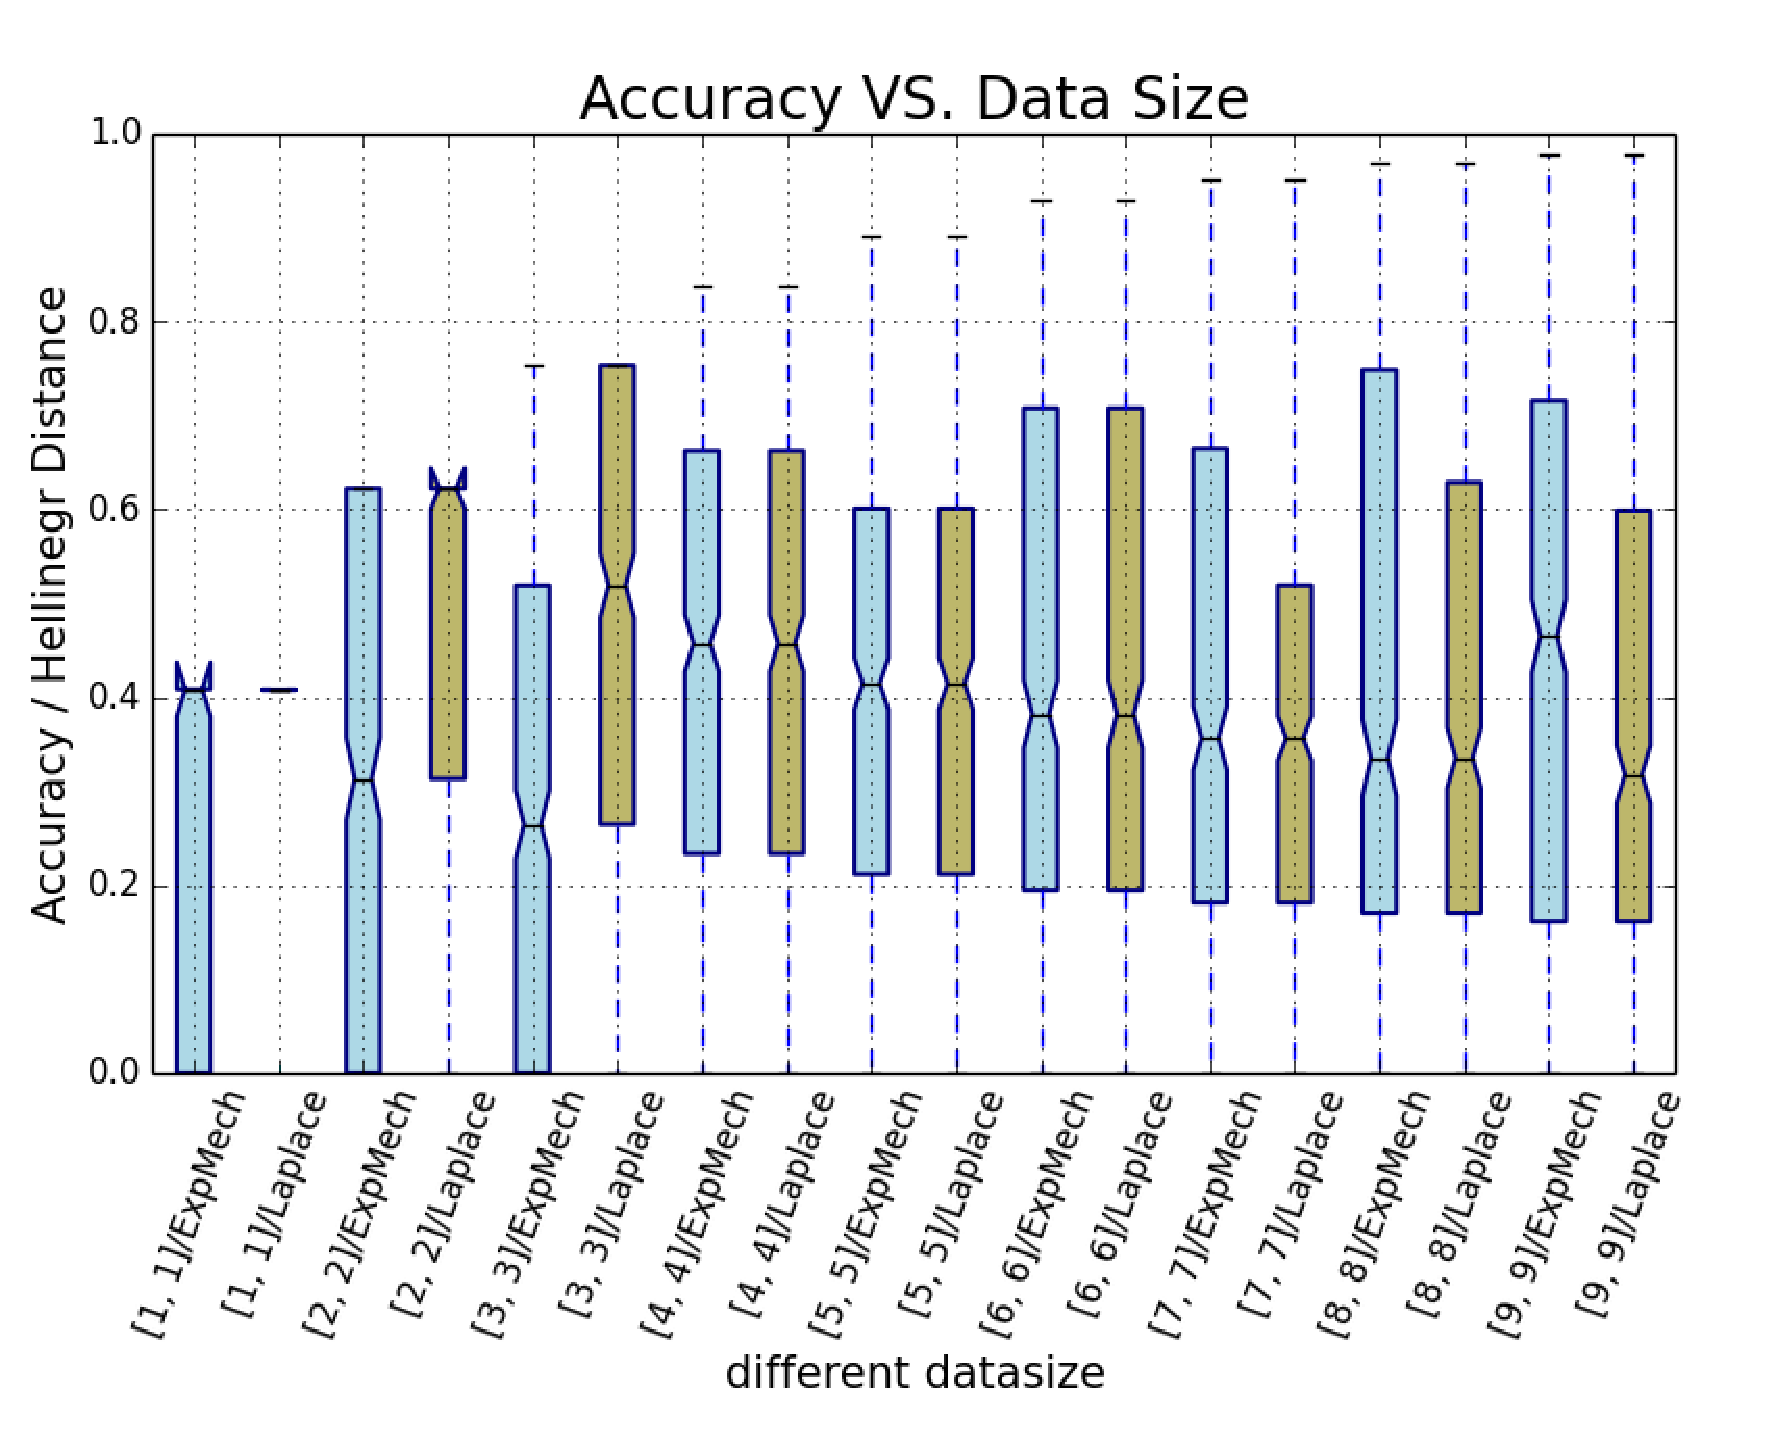
\includegraphics[width=0.3\textwidth]{accuracy_vs_datasize_1_1.eps}}
  \subfigure[three dimensions with $\dirichlet (1,1,1)$ prior distribution]{
    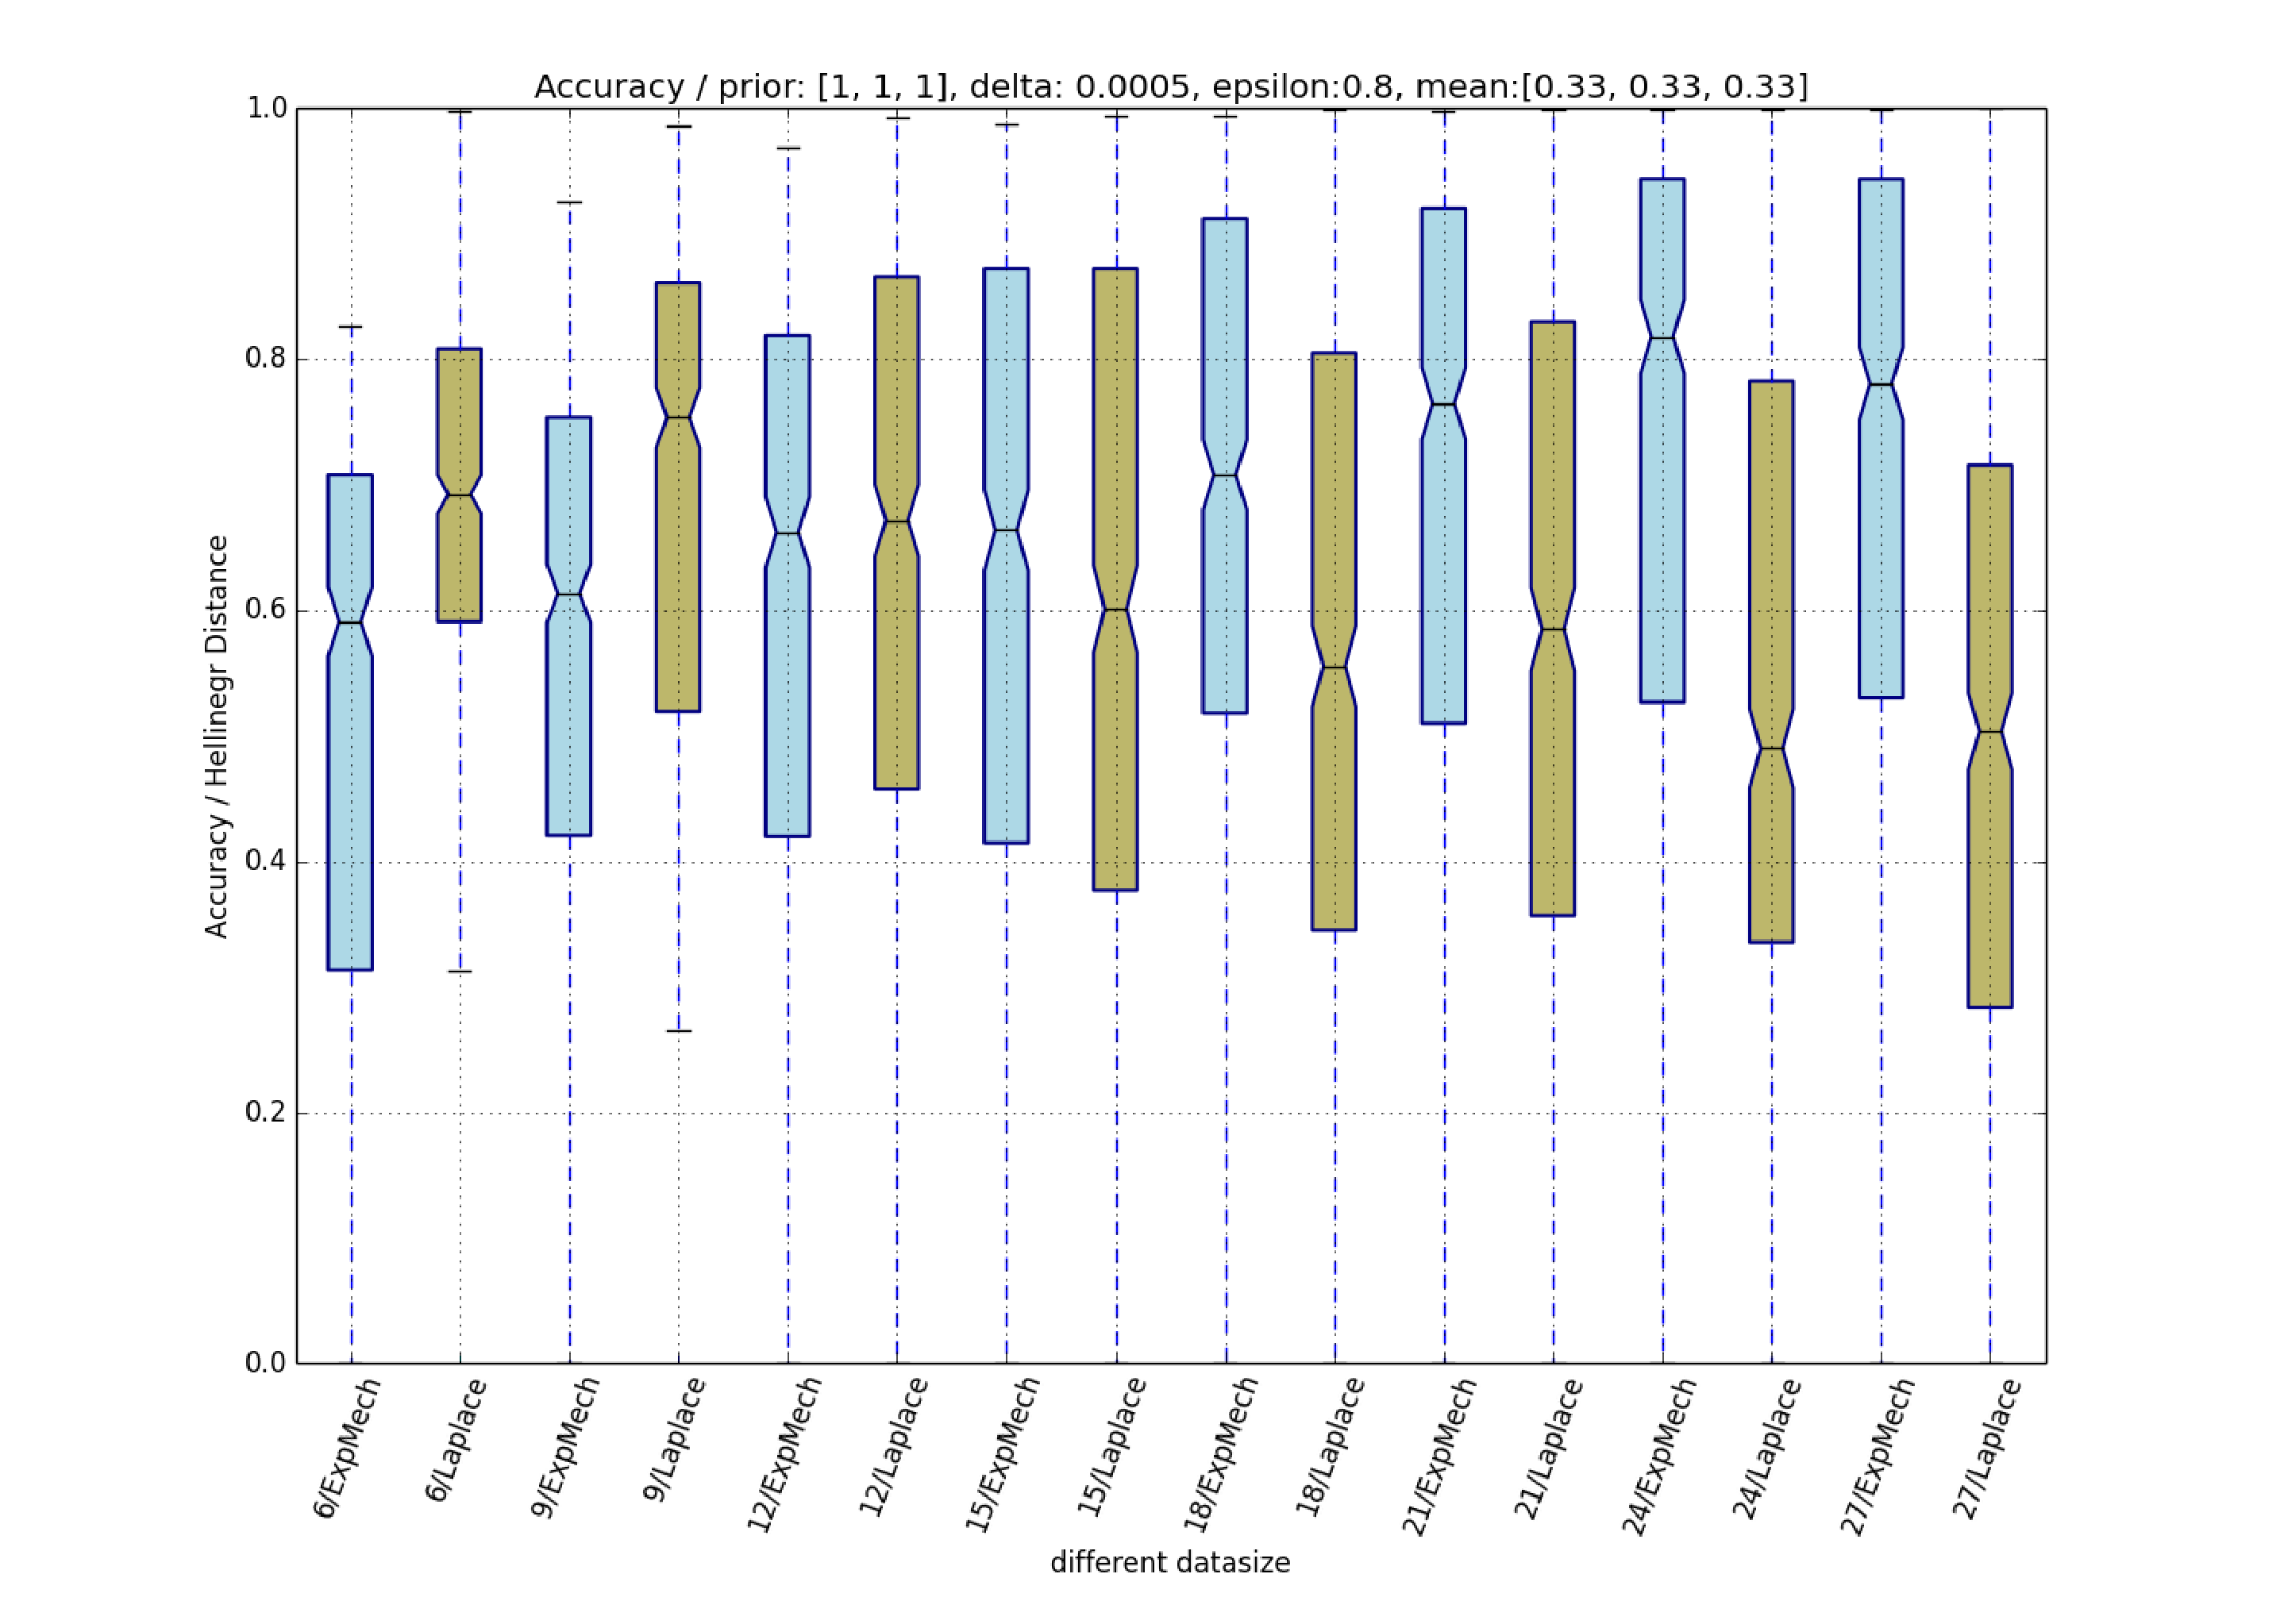
\includegraphics[width=0.3\textwidth]{accuracy_vs_datasize_1_1_1.eps}} 
\caption{Accuracy measurement based on Hellinger distance wrt. different datasizes. Settings: observed data are uniformly distributed, $\epsilon = 0.8$ and $\delta = 0.00000001$}
\label{fig_vs_datasize}
\end{center}
\end{figure}

In Fig. \ref{fig_vs_datasize}, both of the two plots show that when data size go larger, accuracy of our exponential mechanism are decreasing. In Fig. \ref{fig_vs_datasize}(a), when the data size is smaller than 12, we can beta Laplace mechanism but fail when data size larger than or equal to 12. Same as in Fig. \ref{fig_vs_datasize}(b), we can beat Laplace mechanism when data size is smaller than 15 and fail otherwise.

\subsubsection{Accuracy Evaluation wrt. Dimensions}
\label{subsubsec_vs_dimension}


\begin{figure}[ht]
\centering
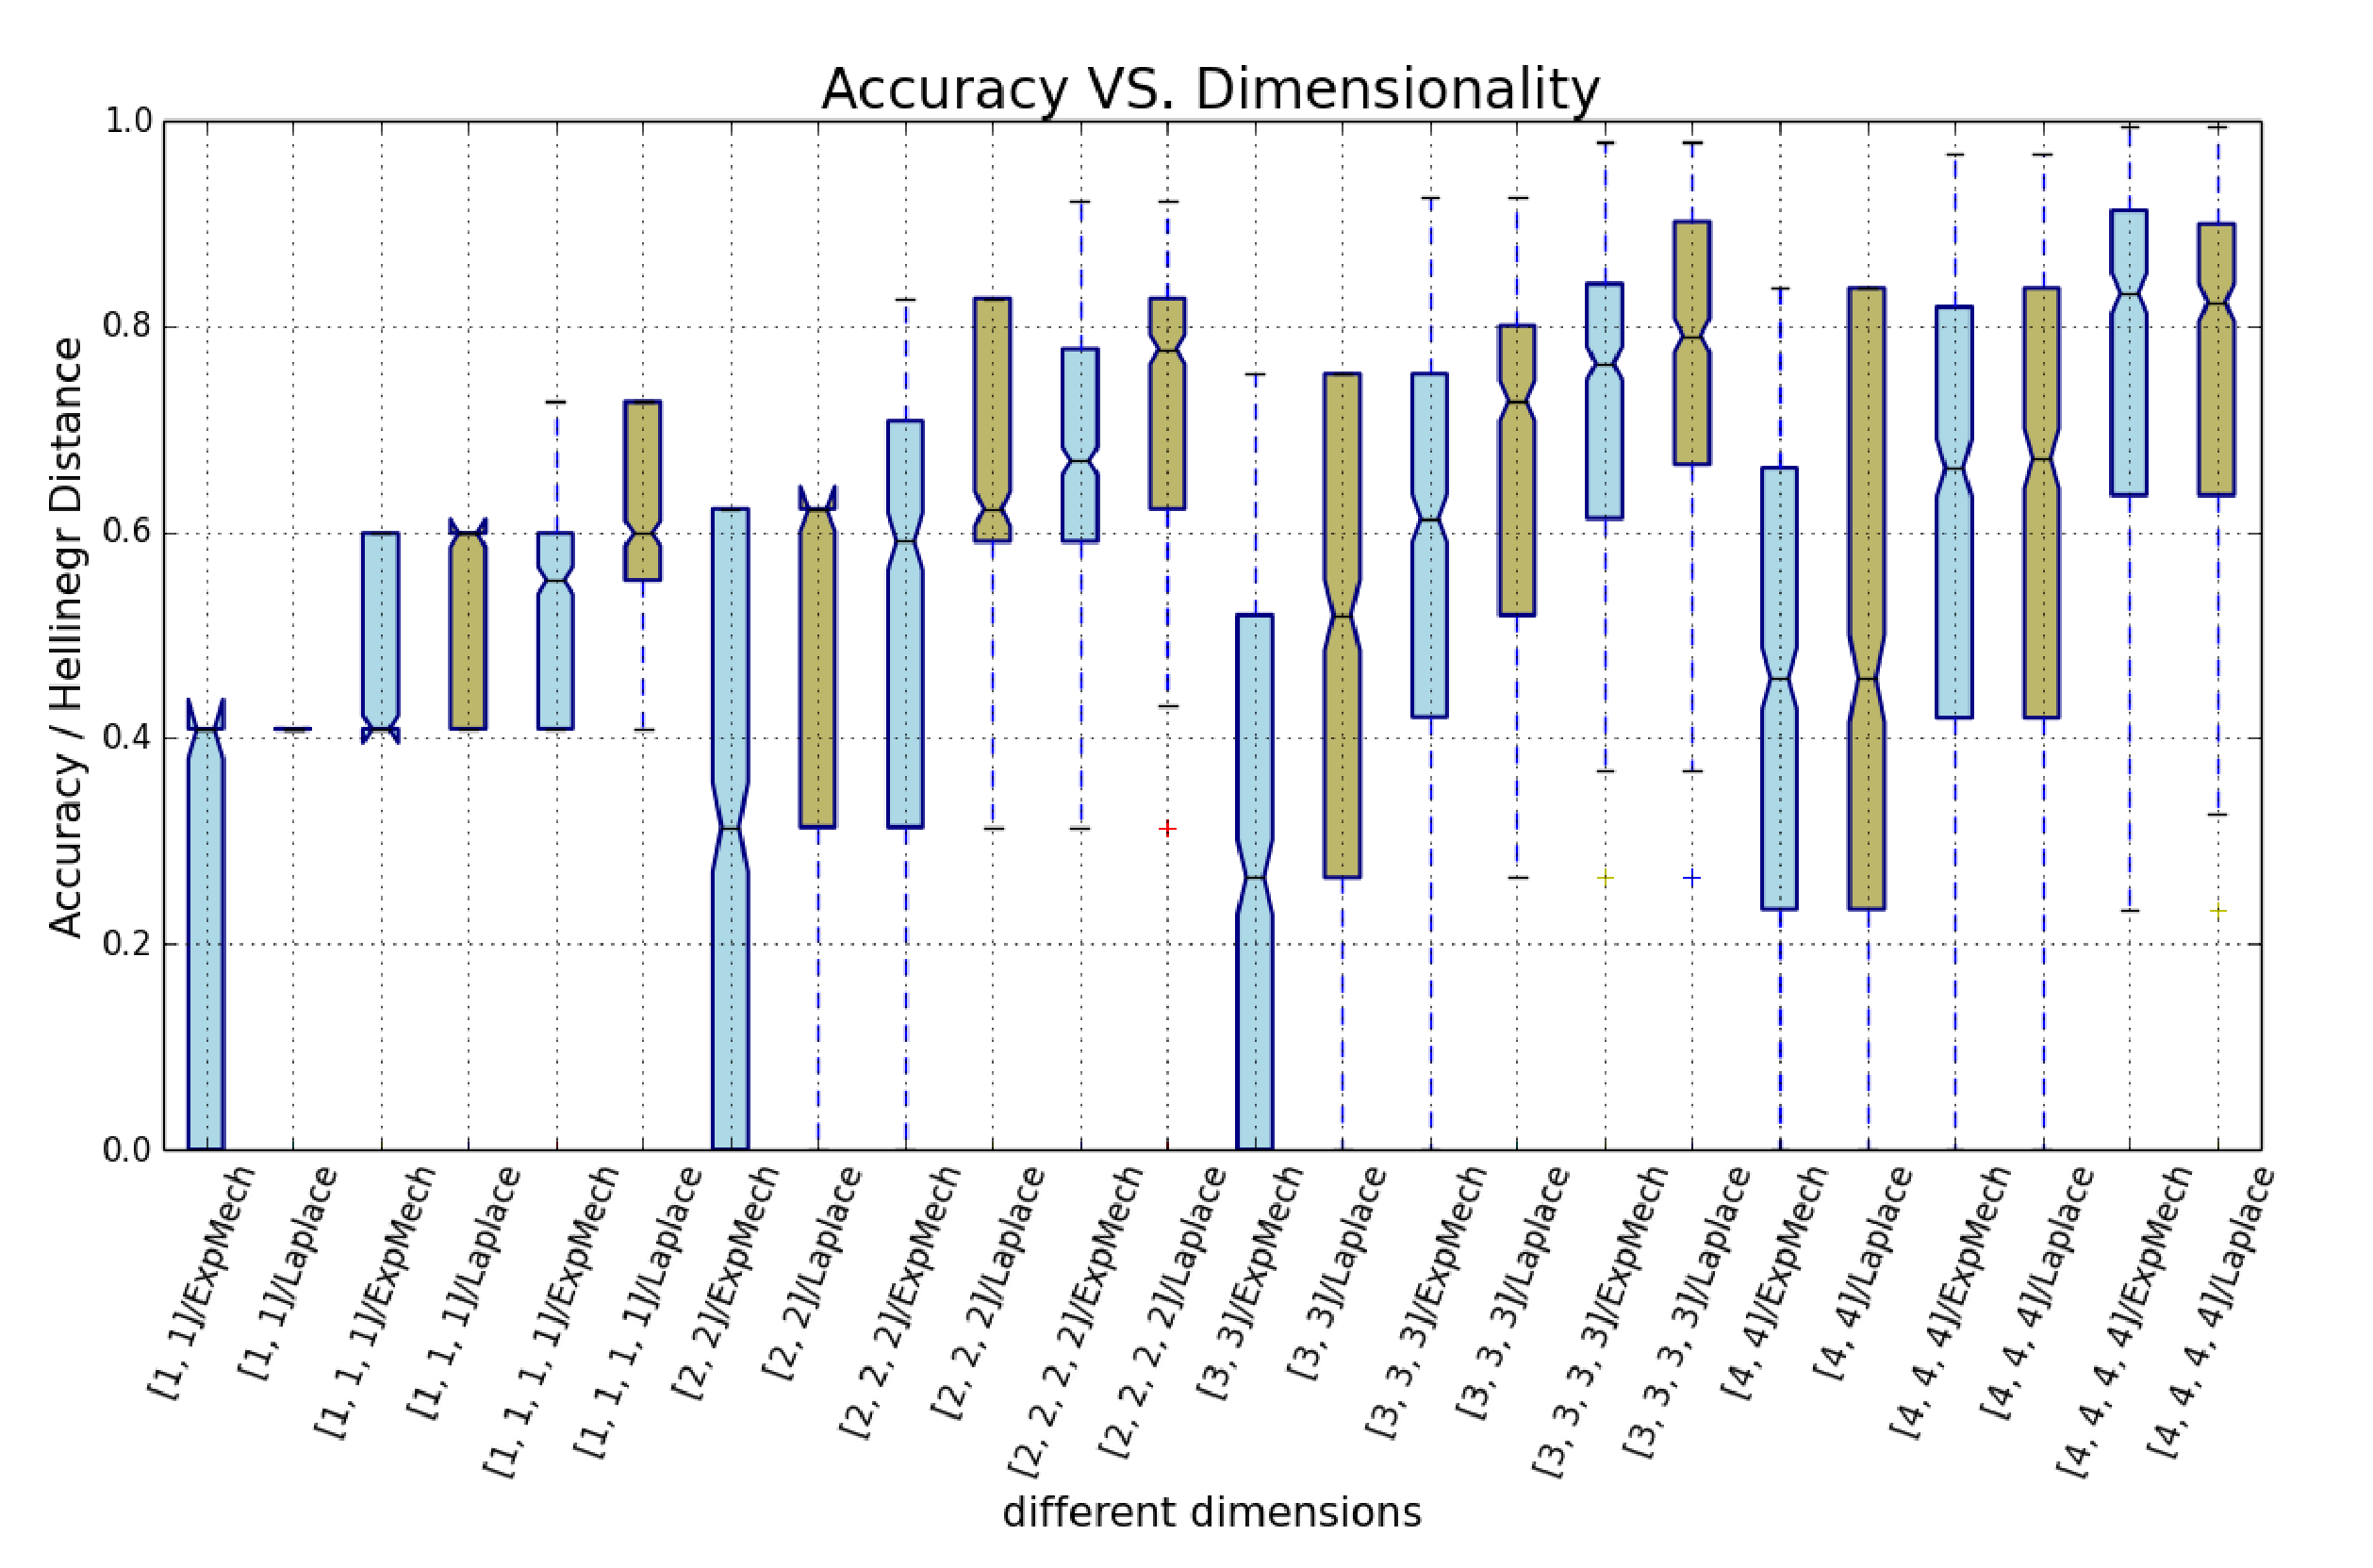
\includegraphics[width=0.45\textwidth]{accuracy_vs_dimension.eps}
\caption{Accuracy measurement based on Hellinger distance wrt. different dimensions and data size. Settings: observed data are uniformly distributed, $\epsilon = 0.8$ and $\delta = 0.00000001$, prior distributions are all $1$ in every dimension}
\label{fig_vs_dimension}
\end{figure}

In Fig. \ref{fig_vs_dimension}, x-axis are observed data sets of different size and dimensions. The plot shows that dimensions have similar influence on our exponential mechanism and the Laplace mechanism. Accuracy of two mechanisms both decrease when dimensions go larger. We will be beat by Laplace mechanism when data size increase but will not be affected when dimensions increase. In other words, dimension has little influence on whether we will beat Laplace mechanism.


\subsubsection{Accuracy Evaluation wrt. Data variance}
\label{subsubsec_vs_variance}

\begin{figure}[ht]
\centering
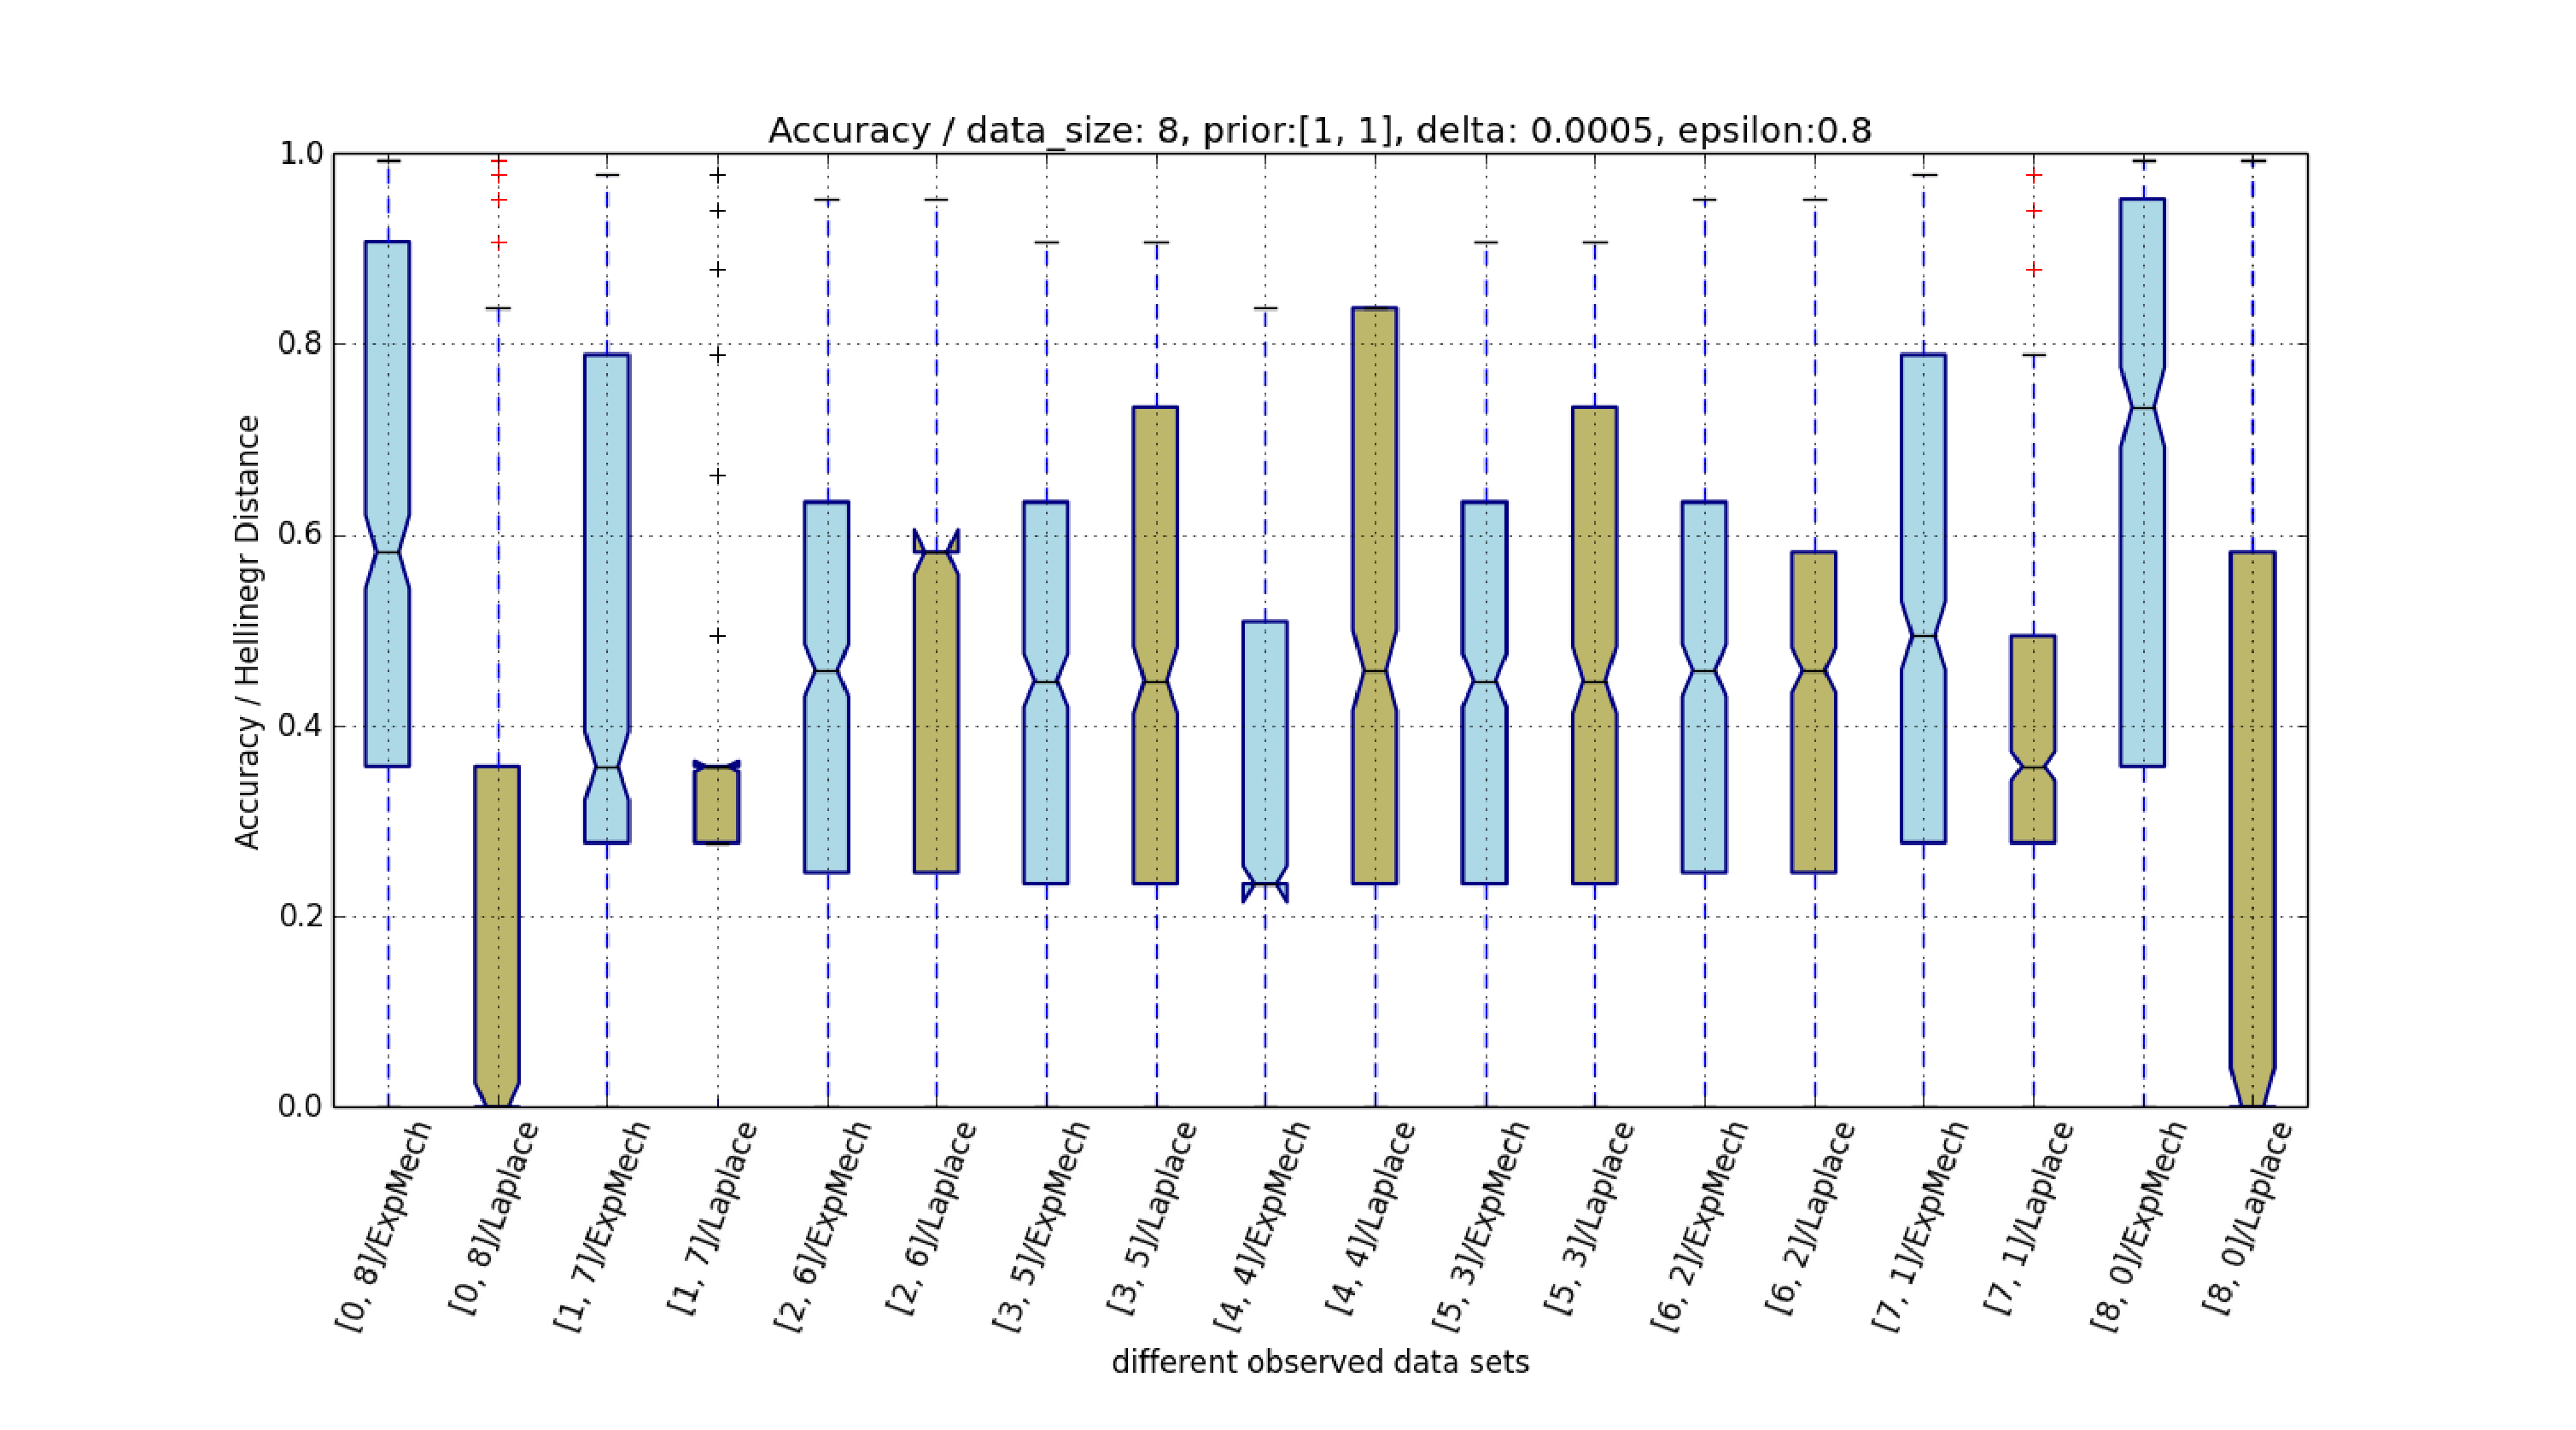
\includegraphics[width=0.45\textwidth]{accuracy_vs_mean_1_1.eps}
\caption{Accuracy measurement based on Hellinger distance wrt. different data variance. Settings: $\epsilon = 0.8$ and $\delta = 0.00000001$, prior distributions are all $1$ in every dimension}
\label{fig_vs_variance}
\end{figure}

In Fig. \ref{fig_vs_variance}, x-axis are observed data sets of different variances (or means). We study this variable under two-dimension $\betad$ distribution in order to be concise. It shows that our mechanism's accuracy is better when data variance go smaller, meanwhile Laplace mechanism go worse. We will beat Laplace mechanism when observed data are more uniformly.



\subsubsection{Accuracy Evaluation wrt. Prior Distribution}
\label{subsubsec_vs_prior}

\begin{figure}[ht]
\centering
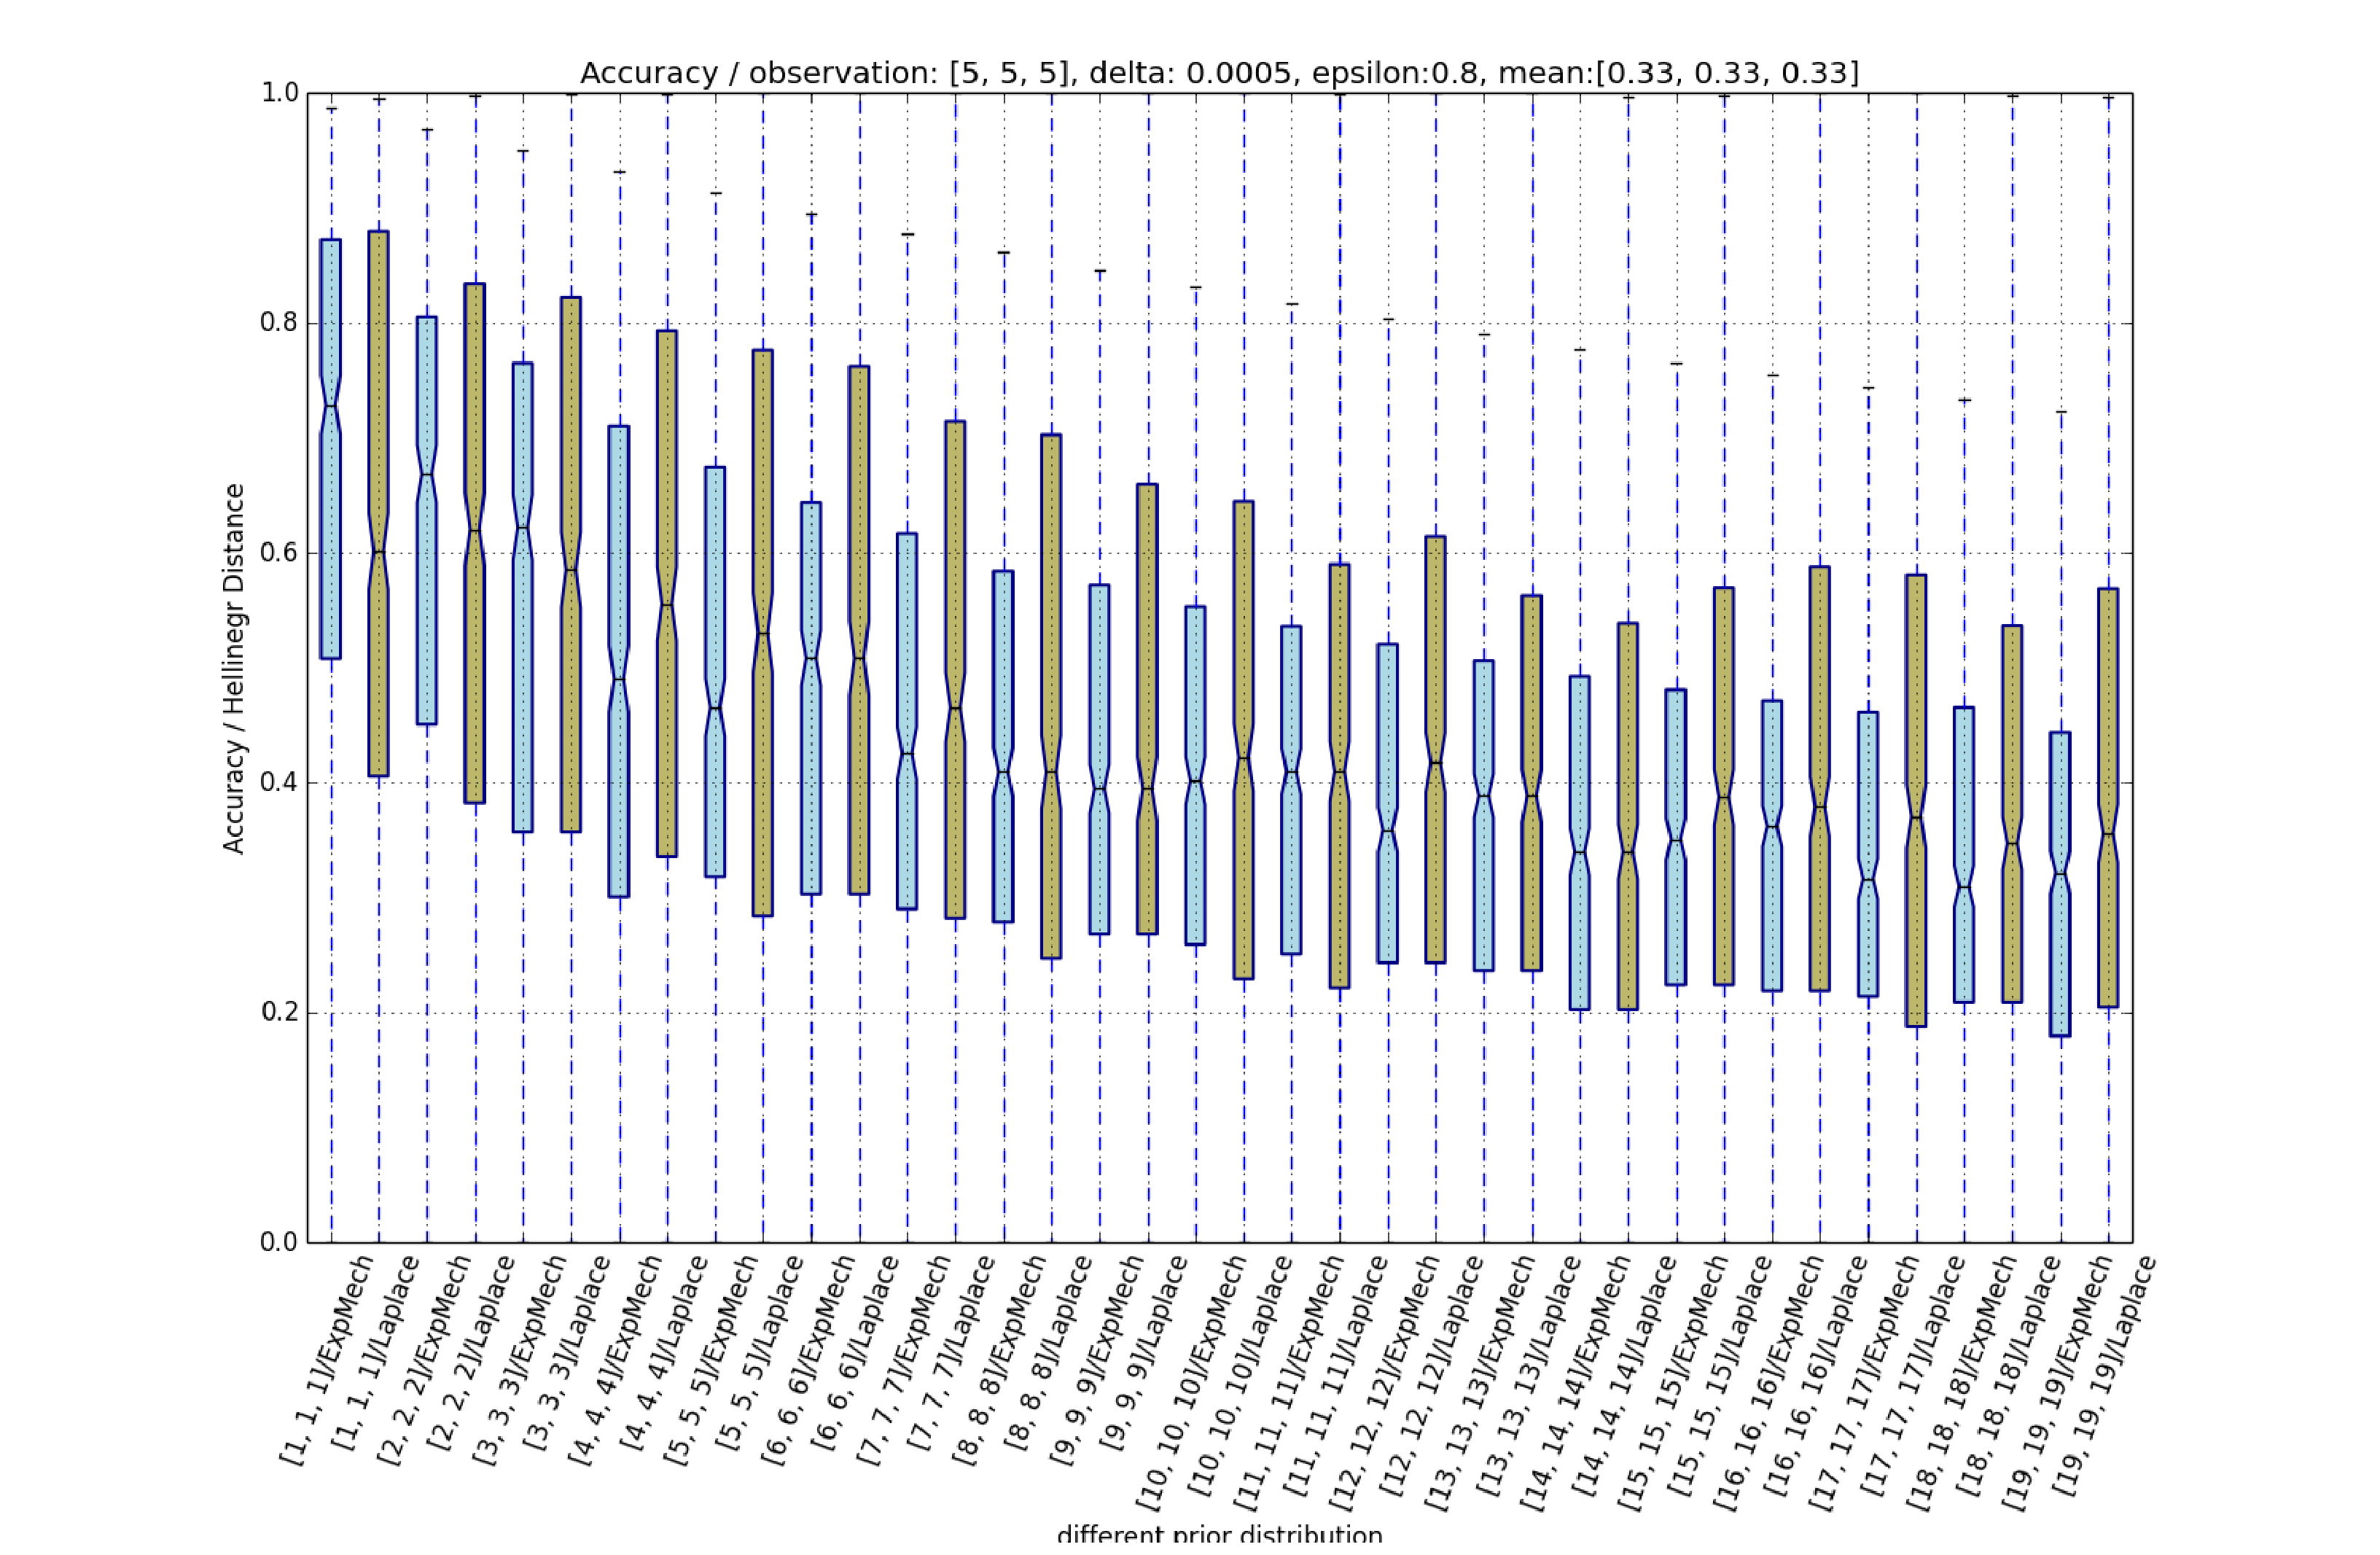
\includegraphics[width=0.45\textwidth]{accuracy_vs_prior_5_5_5.eps}
\caption{Accuracy measurement based on Hellinger distance wrt. different prior distribution. Settings: $\epsilon = 0.8$ and $\delta = 0.00000001$, observed data set is: $[5,5,5]$}
\label{fig_vs_prior}
\end{figure}

In Fig. \ref{fig_vs_prior}, we study this variable under setting that observed data set is $[5,5,5]$ because in Fig. \ref{fig_vs_datasize} Laplace mechanism beat us when data size is 15 and uniformly distributed. The plot shows that in the beginning we cannot beat Laplace but when prior distribution grow larger, we perform better and better and beat Laplace mechanism finally.



% \subsubsection{Accuracy Evaluation wrt. Prior Distribution and Data Variance}
% \label{subsubsec_vs_prior_variance}

% \begin{figure}[ht]
% \centering
% 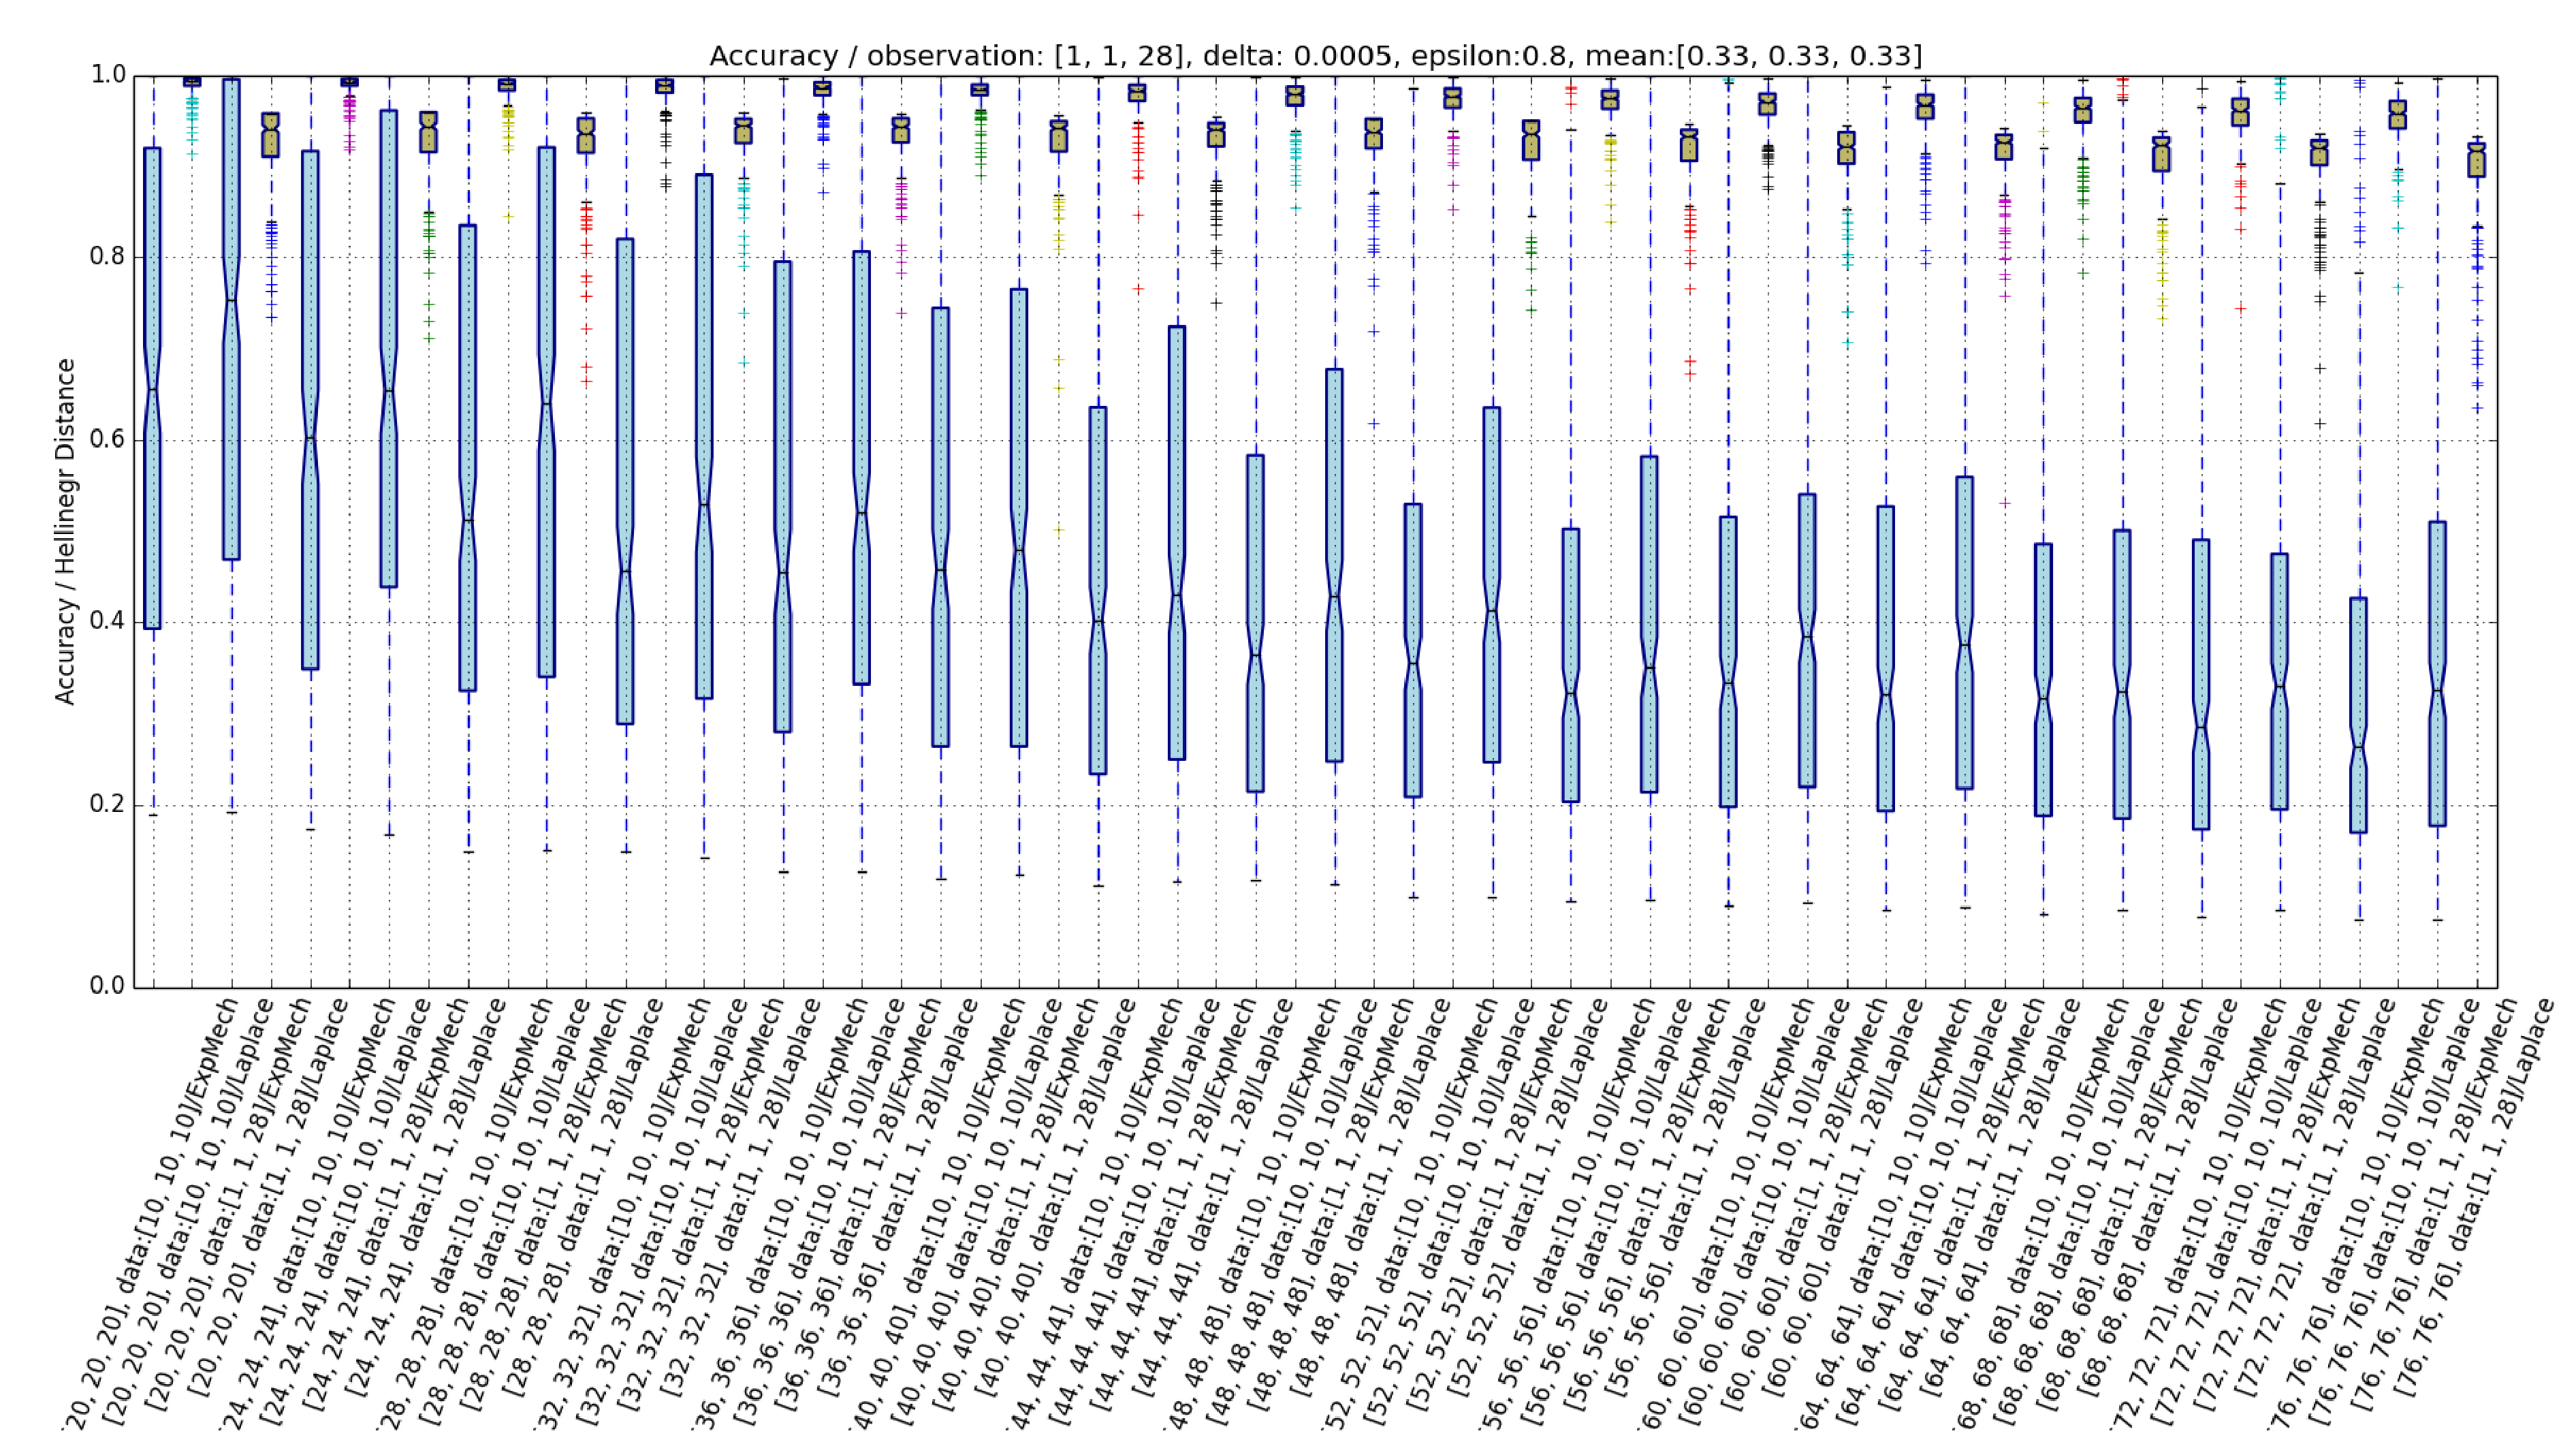
\includegraphics[width=0.45\textwidth]{Accuracy_VS_Prior_mean.eps}
% \caption{Accuracy measurement based on Hellinger distance wrt. different prior distribution and data variances. Settings: $\epsilon = 0.8$ and $\delta = 0.00000001$, observed data sets are $[10,10,10]$ and $[1,1,28]$ and prior distributions are range from $[20,20,20]$ to $[76,76,76]$}
% \label{fig_vs_prior_variance}
% \end{figure}

% Here, we change the prior distribution and data variance in the same time. As shown in Fig. \ref{fig_vs_prior_variance}, our exponential mechanism do better in uniform data set than in edging data set while Laplace mechanism on the contrary. Moreover, our mechanism is improving continuously and significantly as prior distribution increasing while Laplace mechanism isn't.


\section{Conclusions}
We can obtain some preliminary conclusions: 
\begin{enumerate}
	\item We can beat Laplace mechanism when data size is small.
	\item We will beat Laplace mechanism when observed data are more uniformly.
  \item When prior distribution grow larger, we perform better and better and beat Laplace mechanism finally.
\end{enumerate} 

In consequence, we have a better accuracy in small data size, in larger prior and in uniformly data.



\bibliographystyle{ACM-Reference-Format}
\bibliography{bayesian.bib}

\end{document}
 % TODO: replace with your brilliant paper!
% 
%packages
\usepackage{natbib}
\usepackage{amsmath}
\usepackage{amsthm}
\usepackage{mathtools}
\usepackage{mdframed}
\usepackage{subfigure}
\usepackage{booktabs}
% \usepackage{hyperref}
\usepackage{subfigure}
\usepackage{siunitx} % Provides the \SI{}{} and \si{} command for typesetting SI units
\usepackage{graphicx} % Required for the inclusion of images
% \usepackage{natbib} % Required to change bibliography style to APA
\usepackage{datetime}
\usepackage{lscape}
\usepackage{algorithm}
\usepackage{algorithmic}
\usepackage{xspace}
\usepackage[english]{babel} % English language/hyphenation
\usepackage{proof}
\usepackage{booktabs} % Top and bottom rules for tables
\usepackage[colorlinks, allcolors = blue,]{hyperref}
\usepackage{accents}
\usepackage{amsfonts}
\usepackage{stmaryrd}
\usepackage{amsmath,amsthm,amssymb,latexsym} 
\usepackage{microtype}
\usepackage{graphicx}
\usepackage{subfigure}
\usepackage{booktabs} % for professional tables
\usepackage{hyperref}
\usepackage{icml2019}
\usepackage{lipsum}

\usepackage{authblk}


%new commands
\newcommand{\theHalgorithm}{\arabic{algorithm}}
\newtheorem{definition}{Definition}
\usepackage{cancel}
\usepackage[normalem]{ulem}
\newcommand{\dataobs}{\textbf{x}}
\newcommand{\adj}[2]{\textbf{adj}(#1,#2)}
\newcommand{\candidateset}{\mathcal{R}_{\textup{post}}}
\newcommand{\bprior}{\boldsymbol{\beta}_{\textup{prior}}}
\newcommand{\bysinfer}{\mathsf{Infer}}
\newcommand{\betad}{\mathsf{Beta}}
\newcommand{\betaf}{\textup{B}}
\newcommand{\mbetaf}{\boldsymbol{\textup{B}}}
\newcommand{\vtheta}{\boldsymbol{\theta}}
\newcommand{\valpha}{\boldsymbol{\alpha}}
\newcommand{\vbeta}{\boldsymbol{\beta}}
\newcommand{\lapmech}{\mathsf{LSDim}}
\newcommand{\ilapmech}{\mathsf{LSHist}}
\newcommand{\binomial}[2]{\mathsf{Bin}(#1, #2)}
\newcommand{\multinomial}[2]{\mathsf{Mult}(#1, #2)}
\newcommand{\expmech}{\mathsf{EHD}}
\newcommand{\hexpmech}{\mathsf{EHDS}}
\newcommand{\lexpmech}{\mathsf{EHDL}}
\newcommand{\hexpmechd}{\mathsf{expMech}^{D}_{\hellinger}}
\newcommand{\privinfer}{\mathsf{PrivInfer}}
\newcommand{\hlg}{\mathsf{H}}
\newcommand{\dirichlet}[1]{\mathsf{Dir}(#1)}
\newcommand{\alphas}{\boldsymbol{\alpha}}
\newcommand{\xis}{\boldsymbol{\xi}}
\newcommand{\iverson}[1]{[#1]}
\newcommand{\datauni}{\mathcal{X}}
\newcommand{\hellinger}{\mathcal{H}}
\newcommand{\ux}[1]{u(\textbf{x}, {#1})}
\newcommand{\uxadj}[1]{u(\textbf{x}', {#1})}
\newcommand{\cardinality}[2]{\mathcal{C}^{#1}_{#2}}
\newcommand{\range}{\mathcal{O}}
\newcommand{\nomalizer}[1]{\sum\limits_{r'\in \mathcal{R}_{\textup{post}}} \exp \big(\frac{-\epsilon\cdot \mathcal{H} (\mathsf{BI}(#1),r')}{4 \cdot S(#1)}\big)}

\newcommand{\unomalizer}[1]{\sum\limits_{r'\in \mathcal{R}_{\textup{post}}} \exp \big(\frac{-\epsilon\cdot u(#1, r')}{4 \cdot S(#1)}\big)}


\newcommand{\hexpmechPr}[2]{\underset{z \thicksim \hexpmech(#1)}{\Pr}\left[ #2 \right]}
\newcommand{\lapmechPr}[2]{\underset{z \thicksim \lapmech(#1)}{\Pr}\left[ #2 \right]}

\newcommand{\ilapmechPr}[2]{\underset{
{z \thicksim \ilapmech(#1)}
}{\Pr}\left[ #2 \right]}

\newtheorem{thm}{Theorem}[section]

\newtheorem{lem}{Lemma}[section]

\newtheorem{assert}{Assertion}[lem]
\newcommand{\lap}[2]{\mathsf{Lap}(#1, #2)}
\newcommand{\todo}[1]{{\footnotesize \color{red}\textbf{[[ #1 ]]}}}

\section{Bayesian Inference Background}
\label{sec_background}
Given a prior belief $\Pr(\theta)$ on some parameter $\theta$,
and given an observation $\dataobs$,
the posterior distribution on $\theta$ given $\dataobs$ is computed as:
\[
  \Pr(\theta | \dataobs) = \frac{\Pr(\dataobs | \theta) \cdot \Pr(\theta)}{\Pr(\dataobs)}
\]
where the expression  $\Pr(\dataobs | \theta)$ denotes the \emph{likelihood} of $\theta$ when
$\dataobs$ is observed. Since we consider $\dataobs$ to be fixed the likelihood is a function of $\theta$.
For the same reason $\Pr(\dataobs)$ is a constant independent of $\theta$.
Usually in statistics the prior distribution $\Pr(\theta)$ is chosen so that it represents
the initial belief on $\theta$. That is, when no data has been observed. In practice though,
prior distributions and likelihood functions are usually chosen so that the posterior
belongs to the same \emph{family} of distributions. In this case we say that the prior
is conjugate of the likelihood function. Using conjugate priors simplify calculcations and allows
for inference to be performed in a recursive fashion over the data.
In this work we will consider a specific instance of Bayesian inference and one of its generalizations.
Specifically, we will consider the situation where $\theta$ represents the parameter --informally called \emph{bias}--
of a Bernoulli distributed random variable, and its immediate generalization where the parameter $\vtheta$ represents
the the vector of parameters of a categorical distributed random variable.
In the former case the prior distribution over $\theta\in [0,1]$ is going to be a beta distribution, $\betad(\alpha, \beta)$, with parameters
$\alpha,\beta\in\mathbb{R}^{+}$, and with p.d.f:
\[
  \Pr(\theta)\equiv \frac{\theta^{\alpha} (1- \theta)^{\beta}}{\betaf(\alpha,\beta)}
\]
where $\betaf(\cdot,\cdot)$ is the beta function.
The data $\dataobs$ will be a sequence of $n\in\mathbb{N}$ binary values, that is $\dataobs=\langle x_1,\dots x_n \rangle, x_i\in\{0,1\}$, and the likelihood function is:
\[
  \Pr(\dataobs | \theta)\equiv \theta^{\Delta \alpha}(1-\theta)^{n - \Delta \alpha}
\]
where $\Delta \alpha = \displaystyle\sum_{i=1}^{n}x_i$.
From this it can easily be derived that the posterior distribution is:
\[
  \Pr(\theta|\dataobs)=\betad(\alpha + \Delta \alpha,\beta + n - \Delta \alpha)
\]
In the latter case the prior distribution over $\vtheta\in [0,1]^{k}$ is given by a Dirichelet distribution, $\dirichlet(\valpha)$, for $k\in\mathbb{N}$,
and $\valpha\in(\mathbf{R^{+}})^{k}$, with p.d.f:
\[
  \Pr(\vtheta)\equiv\frac{1}{\mbetaf(\valpha)}\cdot \displaystyle\prod_{i=1}^{k}{\theta_i^{\alpha_i-1}}
\]
where $\mbetaf(\cdot)$ is the generealised beta function.
The data $\dataobs$ will be a sequence of $n\in\mathbb{N}$ values coming from a universe $\datauni$, such that $\mid\datauni \mid=k$.
The likelihood function will be:
\[
  \Pr(\dataobs|\vtheta)\equiv \displaystyle\prod_{a_i\in\datauni}\theta_{i}^{\Delta \alpha_i},
\]
with $\Delta \alpha_i=\displaystyle\sum_{j=1}^{n}\iverson{x_j=a_i}$, where in $\iverson{\cdot}$ we use
Iverson bracket notation. Denoting by $\Delta\valpha$ the vector $\langle  \Delta\alpha_1,\dots \Delta\alpha_k \rangle$ the posterior distribution over $\vtheta$ turns out to be
\[
  \Pr(\vtheta|\dataobs)=\dirichlet(\valpha+\Delta \valpha). 
\]
where $+$ denotes the component wise  sum of vectors of reals. 


\section{The Problem and Baseline approach}
\label{sec:base}
We are interested in designing a mechanism for privately releasing
\emph{fully} the posterior distributions derived in section \ref{sec_background},
and not a sample from them.  It's worth noticing that the posterior
distributions are fully characterized by their parameters, and the
family (beta, Dirichlet) they belong to.  Hence, in case of the
Beta-Binomial model we are interested in releasing a private version
of the pair of parameters $(\alpha',\beta')=(\alpha + \Delta \alpha,\beta + n - \Delta \alpha)$, and
in the case of the Dirichlet-Multinomial model we are interested in a
private version of $\valpha'=(\valpha + \Delta \valpha)$. \citet{zhang2016differential} and \citet{xiao2012bayesian} have
already attacked this problem and their solution consisted in adding
independent Laplacian noise to the parameters of the posteriors. That
is, in the case of the Beta-Binomial system the value released would
be: $(\tilde\alpha,\tilde\beta)=(\alpha + \Delta \tilde\alpha,\beta + n - \Delta \tilde\alpha)$ where $\Delta \tilde\alpha\sim Lap(\Delta \alpha, \frac{2}{\epsilon})$, and
%with truncating method come from algorithm designed by \citet{zhang2016differential}
where $Lap(\mu,\nu)$
denotes a Laplacian random variable with mean $\mu$ and scale $\nu$.
This mechanism is $\epsilon$-differentially private, and the noise is
calibrated w.r.t. to a sensitivity of 2 which is derived by using
$\ell_1$ norm over the pair of parameters. Indeed, considering two
adjacent\footnote{Given $\dataobs, \dataobs'$  we say that $\dataobs$ and $\dataobs'$ are adjacent and we write, $\adj{\dataobs}{\dataobs'}$, iff\\
$\displaystyle \sum_{i}^{n}\iverson{x_i = x'_i }\leq 1$. } data observations
$\dataobs, \dataobs'$, that, from a unique prior, give rise to two posterior
distributions, characterized by the pairs
$(\alpha',\beta')$ and $(\alpha'',\beta'')$ then
$|\alpha'-\alpha''|+|\beta'-\beta''|\leq 2$.
This argument extends similarly to the Dirichelet-Multinomial system.


\noindent Also, in previous works, the accuracy has been measured again with respect to
$\ell_1$ norm. That is, an upper bound has been given to
\[
  \Pr[|\alpha - \tilde\alpha| + |\beta - \tilde\beta |\geq \gamma ]
\]
where $(\alpha, \beta), (\tilde\alpha,\tilde\beta)$ are as  defined above.
In this work we will use a metric based on a different norm to compute the sensitivity
and provide guarantees on the accuracy. In particular we will consider a metric
over probability measures and not over the parameters that represent them.
Specifically, we will use the Hellinger distance $\hellinger(\cdot,\cdot)$. Given two beta distributions
$\boldsymbol{\beta}_1=\betad(\alpha_1, \beta_1),$ and $\boldsymbol{\beta}_2=\betad(\alpha_2, \beta_2)$ the following equality holds 
\[
  \hellinger(\boldsymbol{\beta}_1, \boldsymbol{\beta}_2)=
  \sqrt{1 - \frac{\betaf(\frac{\alpha_1 + \alpha_2}{2}, \frac{\beta_1 + \beta_2}{2})}{\sqrt{\betaf(\alpha_1,\beta_1)\betaf(\alpha_2,\beta_2)}}}
\]
The same change of metric will be applied to the experimental accuracy guarantees.
% \section{Technical Problem Statement}
% \label{sec_bayesInfer}
% The posterior belief about parameters $\xis$ is inferred from the
% group of sensitive data. Because it is usually published in form of a
% distribution, for example, $\betad(\alpha',\beta'), \cdots,$ itself
% can relieve a lot of information about sensitive data. So, the
% sensitive information we want to protect here is the posterior belief,
% i.e., $Pr(\xis | \dataobs)$, rather than just a sample drew from
% it\cite{foulds2016theory}. Then it will be better if we can use a
% distance over two distributions to measure the accuracy than a
% distance over just parameters or values when we are protecting a
% distribution, for instance, Hellinger distance in our paper. When we
% measure the accuracy between true posterior and protected posterior
% using Hellinger distance, it would be better we can have a protection
% mechanism based on Hellinger distance. However, current mechanisms are
% mainly based on $l_1$ norm by Laplace mechanism
% \cite{zhang2016differential} \cite{xiao2012bayesian}. That's why we
% design our exponential mechanism over Hellinger distance to protect
% the whole posterior distribution.


% \section{Baseline Approach - Laplace Mechanism}
% \label{sec_lap}
% Our baseline approach come from the algorithm designed by \citet{zhang2016differential} that adding Laplace noise (\citet{dwork2014algorithmic}) to posterior parameters to preserve privacy. They perturbed the parameter updates of $\betad$ distribution from Bayesian inference and truncated to rule out invalid $\betad$ parameters to get the protected posteriors.
% Furthermore, we extend their algorithm to the case of $m$ dimensional Dirichlet distributions, where we add $(m-1)$ i.i.d. Laplace noises $\{Lap_1 , Lap_2, \cdots, Lap_{m-1} \}$ and truncate in the same way. 
% %where $Lap_i = floor(Y)$, $Y \sim Lap(\frac{2}{\epsilon})$. 
% The private posterior is $\dirichlet(\valpha + \Delta \valpha')$, where $\Delta \valpha'$ is the perturbed parameter updates.

\section{Our Approach - Exponential Mechanism with Smooth Sensitivity}
\label{sec_smoo}
Given a prior distribution $\bprior=\betad(\alpha, \beta)$ and a sequence of $n$ observations $\dataobs\in\{0,1\}^n$,
we define the follwing set:

\[
  \betaset\equiv\{\betad(\alpha',\beta')\mid \alpha'=\alpha+\Delta\alpha, \beta'=\beta+n-\Delta\alpha\}
\]
where $\Delta\alpha$ is as defined in Section \ref{sec_background}.
Notice that $\betaset$ has $n + 1$ elements, and the Bayesian Inference
process will produce an element from $\betaset$ that we denote by
$\bysinfer(\dataobs)$ -- we don't explicitely parametrize the result by the
prior,  which from now on we consider fixed and we denote it by $\bprior$.


We can now define the mechanism $\hexpmech$ which,
given in input a sequence of observations $\dataobs$, $\epsilon>0$ and $\delta>0$,
produces an element $r$ in $\betaset$ with probability: 

\begin{equation*}
\underset{z \thicksim \hexpmech}{\Pr}[z=r] = \frac {exp(\frac{-\epsilon\cdot\hellinger(\bysinfer(\dataobs),r)}{2\cdot S(\dataobs)})}
{\displaystyle\sum_{r\in\betaset} exp(\frac{-\epsilon\cdot\hellinger(\bysinfer(\dataobs),r)}{2\cdot S(\dataobs)})}
\end{equation*}
this mechanism is based on the basic exponential mechanism \cite{talwar}, with $\betaset$ as range and $\hellinger(\cdot,\cdot)$ as scoring function.
The difference is that in this mechanism we don't calibrate the noise w.r.t. to the global sensitivity of the scoring function but w.r.t. to the smooth sensitivity $S(\dataobs)$
-- \citet{nissim2007smooth}-- of $\hellinger(\bysinfer(\dataobs), \cdot)$. The smooth sensitivity is computed as follows:
\begin{equation}
  \label{eq:smooth}
   S(\dataobs)=\max_{\dataobs' \neq \dataobs, \dataobs' \in \{0,1\}^{n}}\bigg \{\Delta_{l}\bigg (\hellinger(\bysinfer(\dataobs'),\cdot)\bigg )\cdot e^{-\gamma\cdot d(\dataobs, \dataobs')}\bigg\}
\end{equation}
 where $d$ is the Hamming distance between two datasets,  $\gamma = \gamma(\epsilon, \delta)$ is a function
 of $\epsilon$ and $\delta$ to be determined later, and where $\Delta_{l}\bigg (\hellinger(\bysinfer(\dataobs'),\cdot)\bigg )$
 denotes the local sensitivity at $\bysinfer(\dataobs')$, or equivalently at $\dataobs'$ --w.r.t. $\ell_1$ norm--of the scoring function used in our mechanism, that is:
 \begin{equation*}
 \Delta_{l}\bigg (\hellinger(\bysinfer(\dataobs'),\cdot)\bigg )=\max_{\dataobs'' \in \datauni^n:\adj{\dataobs'}{\dataobs''}, r\in \betaset}\lvert \hellinger(\bysinfer(\dataobs'), r) - \hellinger(\bysinfer(\dataobs''), r)\rvert
\end{equation*}

This mechanism also extends to the Dirichlet-Multinomial system $\dirichlet(\valpha)$ by rewriting the Hellinger distance as:
\[
  \hellinger(\dirichlet(\valpha_1), \dirichlet(\valpha_2)) = \sqrt{1 - \frac{\betaf(\frac{\valpha_1 + \valpha_2}{2})}{\sqrt{\betaf(\valpha_1) \betaf(\valpha_2)}}},
\]
and by replacing the $\betaset$ with set of posterior Dirichlet distributions candidates. Also, the smooth sensitivity $S(\dataobs)$ in (\ref{eq:smooth}) will be
computed by letting $\dataobs'$ range over all the elements in $\datauni^{n}$ adjacent to $\dataobs$.
Notice that $\betaset$ has $\binom{n + 1}{m - 1}$ elements in this case. We will denote by
$\hexpmechd$ the mechanism for the Dirichlet-Multinomial system.
% In what follows, we will use a correspondence between the probability
%  $\underset{z \thicksim \hexpmech(x)}{Pr}[z = r]$ of every
%  $r\in\betaset$ and the probability 
%  $\underset{z \thicksim \hexpmech(x)}{Pr}[\hlg(\bysinfer(x),z) =
%  \hlg(\bysinfer(x),r)]$ for the utility score for $r$. In particular, for every
%  $r\in\betaset$ we have:
% $$
% \underset{z \thicksim \hexpmech(x)}{Pr}[z = r]=
% \frac{1}{2}\Big (\underset{z \thicksim \hexpmech(x)}{Pr}[\hlg(\bysinfer(x),z) =
%  \hlg(\bysinfer(x),r)]\Big )
% $$
% To see this, it is enough to notice that: $\underset{z \thicksim \hexpmech(x)}{Pr}[z = r]$ is proportional too $\hlg(\bysinfer(x),r)$, i.e., $u(x,z)$. We can derive, if $u(r,x) = u(r',x)$ then $\underset{z \thicksim \hexpmech(x)}{Pr}[z = r] = \underset{z \thicksim \hexpmech(x)}{Pr}[z = r']$. We assume the number of candidates $z \in \mathcal{R}$ that satisfy $u(z,x) = u(r,x)$ is $|r|$, we have  $\underset{z \thicksim \hexpmech(x)}{Pr}[u(z,x) = u(r,x)] = |r| \underset{z \thicksim \hexpmech(x)}{Pr}[z = r]$. Because Hellinger distance  $\hlg(\bysinfer(x),z)$ is axial symmetry, where the $\bysinfer(x)$ is the symmetry axis. It can be infer that $|z| = 2$ for any candidates, apart from the true output, i.e., $\underset{z \thicksim \hexpmech(x)}{Pr}[u(z,x) = u(r,x)] = 2 \underset{z \thicksim \hexpmech(x)}{Pr}[z = r]$. This parameter can be eliminate in both sides in proof.

% In our private Bayesian inference mechanism, we set the $\beta$ as $\ln(1 - \frac{\epsilon}{2 \ln (\frac{\delta}{2 (n + 1)})})$. 
The following result guarantees that the mechanisms are indeed differentially private.

\begin{theorem}[Privacy] 
  For  $\gamma=\ln(1 - \frac{\epsilon}{2 \ln (\frac{\delta}{2 (n + 1)})})$, both
  $\hexpmech$ and $\hexpmechd$ are $(\epsilon,\delta)$-differentially private.
\end{theorem}




% \subsection{Sliding Property of Exponential Mechanism}
% \begin{lem}
% Consider the exponential mechanism  $\sexpmech(x,u,\mathcal{R})$
% calibrated on the smooth sensitivity. Let $\lambda = f(\epsilon,
% \delta)$, $\epsilon\geq 0$ and $|\delta| < 1$. Then, the following \emph{sliding property} holds:
% \begin{equation*}
% \underset{r \thicksim \hexpmech(x)}{Pr}[u(r,x) = \hat{s}]
% \leq
% e^{\frac{\epsilon}{2}} \underset{r \thicksim \hexpmech(x)}{Pr}[u(r,x) = (\Delta + \hat{s})] + \frac{\delta}{2},
% \end{equation*}

% \end{lem}

% \begin{proof}

% We denote the normalizer of the probability mass in $\hexpmech(x)$: $\sum_{r' \in \mathcal{R}}exp(\frac{\epsilon u(r',x)}{2 S(x)})$ as $NL(x)$:
% \begin{equation*}
% \begin{split}
% LHS 
%   = \underset{r \thicksim \hexpmech(x)}{Pr}[u(r,x) = \hat{s}]
% & = \frac{exp(\frac{\epsilon \hat{s}}{2 S(x)})}{NL(x)}\\
% & = \frac{exp(\frac{\epsilon (\hat{s} + \Delta - \Delta)}{2 S(x)})}{NL(x)}\\
% & = \frac{exp(\frac{\epsilon (\hat{s} + \Delta)}{2 S(x)} + \frac{- \epsilon \Delta}{2 S(x)})}{NL(x)}\\
% & = \frac{exp(\frac{\epsilon (\hat{s} + \Delta)}{2 S(x)})}{NL(x)} \cdot e^{\frac{- \epsilon \Delta}{2 S(x)})}.\\
% \end{split}
% \end{equation*}

% By bounding the $\Delta \geq -S(x)$, we can get:

% \begin{equation*}
% \begin{split}
% \frac{exp(\frac{\epsilon (\hat{s} + \Delta)}{2 S(x)})}{NL(x)} \cdot e^{\frac{- \epsilon \Delta}{2 S(x)}}
% & \leq \frac{exp(\frac{\epsilon (\hat{s} + \Delta)}{2 S(x)})}{NL(x)} \cdot e^{\frac{\epsilon}{2}}\\
% &  =  e^{\frac{\epsilon}{2}} \underset{z \thicksim \hexpmech(x)}{Pr}[u(r,x) = (\Delta + \hat{s})] \leq RHS\\
% \end{split}
% \end{equation*}

% \end{proof}

% \subsection{Dilation Property of Exponential Mechanism}
% \begin{lem}
% for any exponential mechanism $\hexpmech(x)$, $\lambda < |\beta|$, $\epsilon$, $|\delta| < 1$ and $\beta \leq \ln(1 - \frac{\epsilon}{2 \ln (\frac{\delta}{2 (n + 1)})})$, the dilation property holds:

% \begin{equation*}
% \underset{z \thicksim \hexpmech(x)}{Pr}[u(z,x) = c]
% \leq
% e^{\frac{\epsilon}{2}} \underset{z \thicksim \hexpmech(x)}{Pr}[u(z,x) = e^{\lambda} c] + \frac{\delta}{2},
% \end{equation*}
% where the sensitivity in mechanism is still smooth sensitivity as above.
% \end{lem}

% \begin{proof}

% The sensitivity is always greater than 0, and our utility function $-\hlg(\bysinfer(x),z)$ is smaller than zero, i.e., $u(z,x) \leq 0$, we need to consider two cases where $\lambda < 0$, and $\lambda > 0$:

% We set the $h(c) = Pr[u(\hexpmech(x)) = c] = 2\frac{exp(\frac{\epsilon z}{2 S(x)})}{NL(x)}$.

% We first consider $\lambda < 0$. In this case, $1 < e ^ {\lambda}$, so the ratio $\frac{h(c)}{h(e^{\lambda}c)} = \frac{exp(\frac{\epsilon c}{2 S(x)})}{exp(\frac{\epsilon (c \cdot e^{\lambda})}{2 S(x)})}$ is at most $\frac{\epsilon}{2}$.

% Next, we proof the dilation property for $\lambda > 0$, The ratio of $\frac{h(c)}{h(e^{\lambda}c)}$ is $\exp(\frac{\epsilon}{2} \cdot \frac{u(\hexpmech(x)) (1 - e^{\lambda})}{S(x)})$. Consider the event $G = \{ \hexpmech(x) : u(\hexpmech(x)) \leq \frac{S(x)}{(1 - e^{\lambda})}\}$. Under this event, the log-ratio above is at most $\frac{\epsilon}{2}$. The probability of $G$ under density $h(c)$ is $1 - \frac{\delta}{2}$. Thus, the probability of a given event $z$ is at most $Pr[c \cap G] + Pr[\overline{G}] \leq e^{\frac{\epsilon}{2}} Pr[e^{\lambda}c \cap G] + \frac{\delta}{2} \leq e^{\frac{\epsilon}{2}} Pr[e^{\lambda}c] + \frac{\delta}{2}$.\\


% \textbf{Detail proof:}
% \begin{itemize}

% 	\item $\lambda < 0$

% 		The left hand side will always be smaller than 0 and the right hand side greater than 0. This will always holds, i.e.
% 		\begin{equation*}
% 		\end{equation*}
% 	\item $\lambda > 0$


% Because $\hat{s} = u(r)$ where $r \thicksim \hexpmech(x)$, we can substitute $\hat{s}$ with $u(\hexpmech(x))$. Then, what we need to proof under the case $\lambda > 0$ is:
% \begin{equation*}
% u(\hexpmech(x)) \leq \frac{S(x)}{(1 - e ^ {\lambda})}
% \end{equation*}
% By applying the accuracy property of exponential mechanism, we bound the probability that the equation holds with probability:
% \begin{equation*}
% \begin{split}
% Pr[u(\hexpmech(x)) \leq \frac{S(x)}{(1 - e ^ {\lambda})}] 
% & \leq \frac{|\mathcal{R}|exp(\frac{\epsilon S(x)}{(1 - e ^ {\lambda})}/2 S(x))}{|\mathcal{R}_{OPT}| exp(\epsilon OPT_{u(x)}/2 S(x))}\\
% \end{split}
% \end{equation*}

% In our Bayesian Inference mechanism, the size of the candidate set $\mathcal{R}$ is equal to the size of observed data set plus 1, i.e., $n + 1$, and $OPT_{u(x)} = 0$, then we have:
% \begin{equation*}
% \begin{split}
% Pr[u(\hexpmech(x)) \leq \frac{S(x)}{(1 - e ^ {\lambda})}] 
% & = (n + 1)exp(\frac{\epsilon S(x)}{(1 - e ^ {\lambda})}/2 S(x))\\
% & = (n + 1)exp(\frac{\epsilon}{2 (1 - e ^ {\lambda})})\\
% \end{split}
% \end{equation*}

% When we set $\lambda \leq \ln(1 - \frac{\epsilon}{2 \ln (\frac{\delta}{2 (n + 1)})})$, it is easily to derive that $Pr[u(\hexpmech(x)) \leq \frac{S(x)}{(1 - e ^ {\lambda})}] \leq \frac{\delta}{2}$.

% \end{itemize}

% \end{proof}

% \subsection{Privacy Analysis}
% \begin{lem}
% \label{lem_hexpmech_privacy}
% $\hexpmech$ is $(\epsilon, \delta)$-differential privacy.
% \end{lem}

% \begin{proof}
% of Lemma \ref{lem_hexpmech_privacy}: For all neighboring $x, y \in D^n$ and all sets $\mathcal{S}$, we need to show that:
% \begin{equation*}
% \underset{z \thicksim \hexpmech(x)}{Pr}[ z \in \mathcal{S}] \leq e^{\epsilon} \underset{z \thicksim \hexpmech(y)}{Pr}[z \in \mathcal{S}] + \delta. 
% \end{equation*}
% Given that $2\Big( \underset{z \thicksim \hexpmech(x)}{Pr}[ z \in \mathcal{S}]\Big) = \underset{z \thicksim \hexpmech(x)}{Pr}[ u(x,z) \in \mathcal{U}]$, let $\mathcal{U}_1 = \frac{u(y,z) - u(x,z)}{S(x)}$, $\mathcal{U}_2 = \mathcal{U} + \mathcal{U}_1$ and $\mathcal{U}_3 = \mathcal{U}_2 \cdot \frac{S(x)}{S(y)} \cdot \ln(\frac{NL(x)}{NL(y)})$. Then,

% \begin{equation*}
% \begin{split}
% 2\Big( \underset{z \thicksim \hexpmech(x)}{Pr}[ z \in \mathcal{S}]\Big)
% & = \underset{z \thicksim \hexpmech(x)}{Pr}[ u(x,z) \in \mathcal{U}]\\
% & \leq e^{\epsilon / 2} \cdot \underset{z \thicksim \hexpmech(x)}{Pr}[ u(x,z) \in \mathcal{U}_2]\\
% & \leq e^{\epsilon} \cdot \underset{z \thicksim \hexpmech(x)}{Pr}[ u(x,z) \in \mathcal{U}_3] + e^{\epsilon/2} \cdot \frac{\delta'}{2}\\
% & = e^{\epsilon} \cdot \underset{z \thicksim \hexpmech(y)}{Pr}[ u(y,z) \in \mathcal{U}] + \delta = 2\Big( e^{\epsilon} \cdot \underset{z \thicksim \hexpmech(x)}{Pr}[ z \in \mathcal{S}] \Big) + \delta\\
% \end{split}
% \end{equation*}

% The first inequality holds by the sliding property, since the $\mathcal{U}_1 \geq -S(x)$. The second inequality holds by the dilation property, since $\frac{S(x)}{S(y)} \cdot \ln(\frac{NL(x)}{NL(y)}) \leq 1 - \frac{\epsilon}{2 \ln (\frac{\delta}{2 (n + 1)})}$.

% \end{proof}

\section{Preliminary Experimental Results}
\label{sec_experiment}
In this section, we evaluate the accuracy of the mechanisms defined in
Section (\ref{sec_smoo}) w.r.t. four variables, including data size, dimensions,
data variance, prior distribution, and some combinations thereof.
Every plot is an average over 1000 runs. In all the experiments we set
$\epsilon = 0.8$, and $\delta = 0.00000001$.

\noindent In the following whiskers-plots, the y-axis shows the accuracy (or equivalently, the error) of the mechanisms.
Accuracy is measured using Hellinger distance. The x-axis, instead shows  one of the previously mentioned
independent variables --or a combination thereof.
The boxes extend from the lower to the upper quartile values of the data, with a line at the median. A notch on the box around the median
is also drawn to give a rough guide to the significance of difference of medians;
The whiskers extend from the box to show the range of the data. 
A blue box in the plots represents the exponential mechanism behaviour,
while the yellow box next to it represents the performance of a variation of the
basic Laplace mechanism presented in Section (\ref{sec:base}) with the same settings: that is $\epsilon, \delta$, data, prior.
The variation considered performs a post processing on the released parameters so that they
are consistent. For instance in the case \todo{more info about the truncation}.
\paragraph{Increasing data size with balanced datasets}
\label{subsubsec_vs_datasize}

\begin{figure}[ht]
\begin{center}
\centering
  \subfigure[two dimensions with $\betad (1,1)$ prior distribution]{
    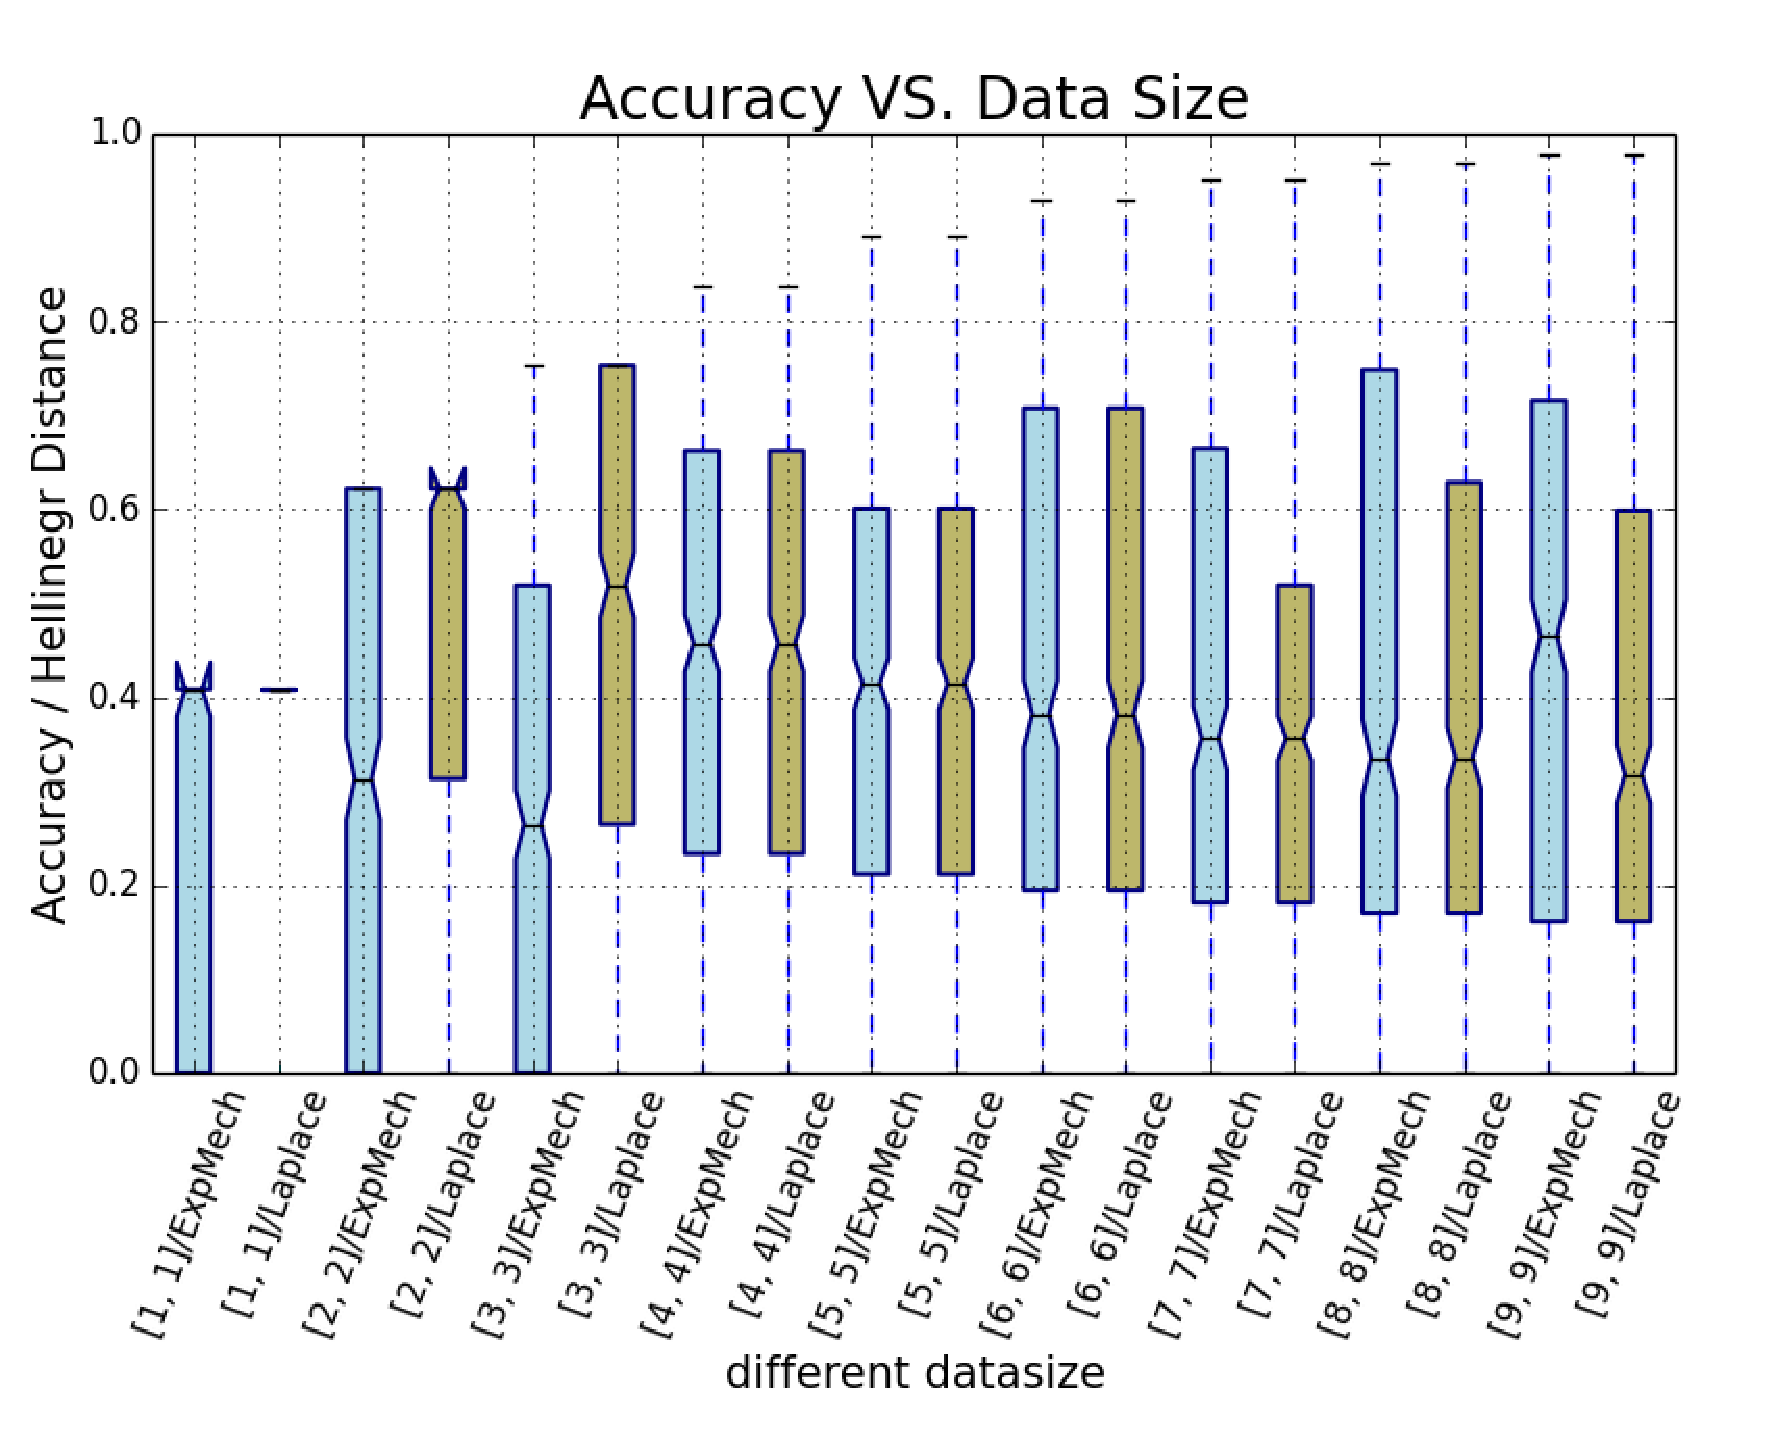
\includegraphics[width=0.3\textwidth]{accuracy_vs_datasize_1_1.eps}}
  \subfigure[three dimensions with $\dirichlet (1,1,1)$ prior distribution]{
    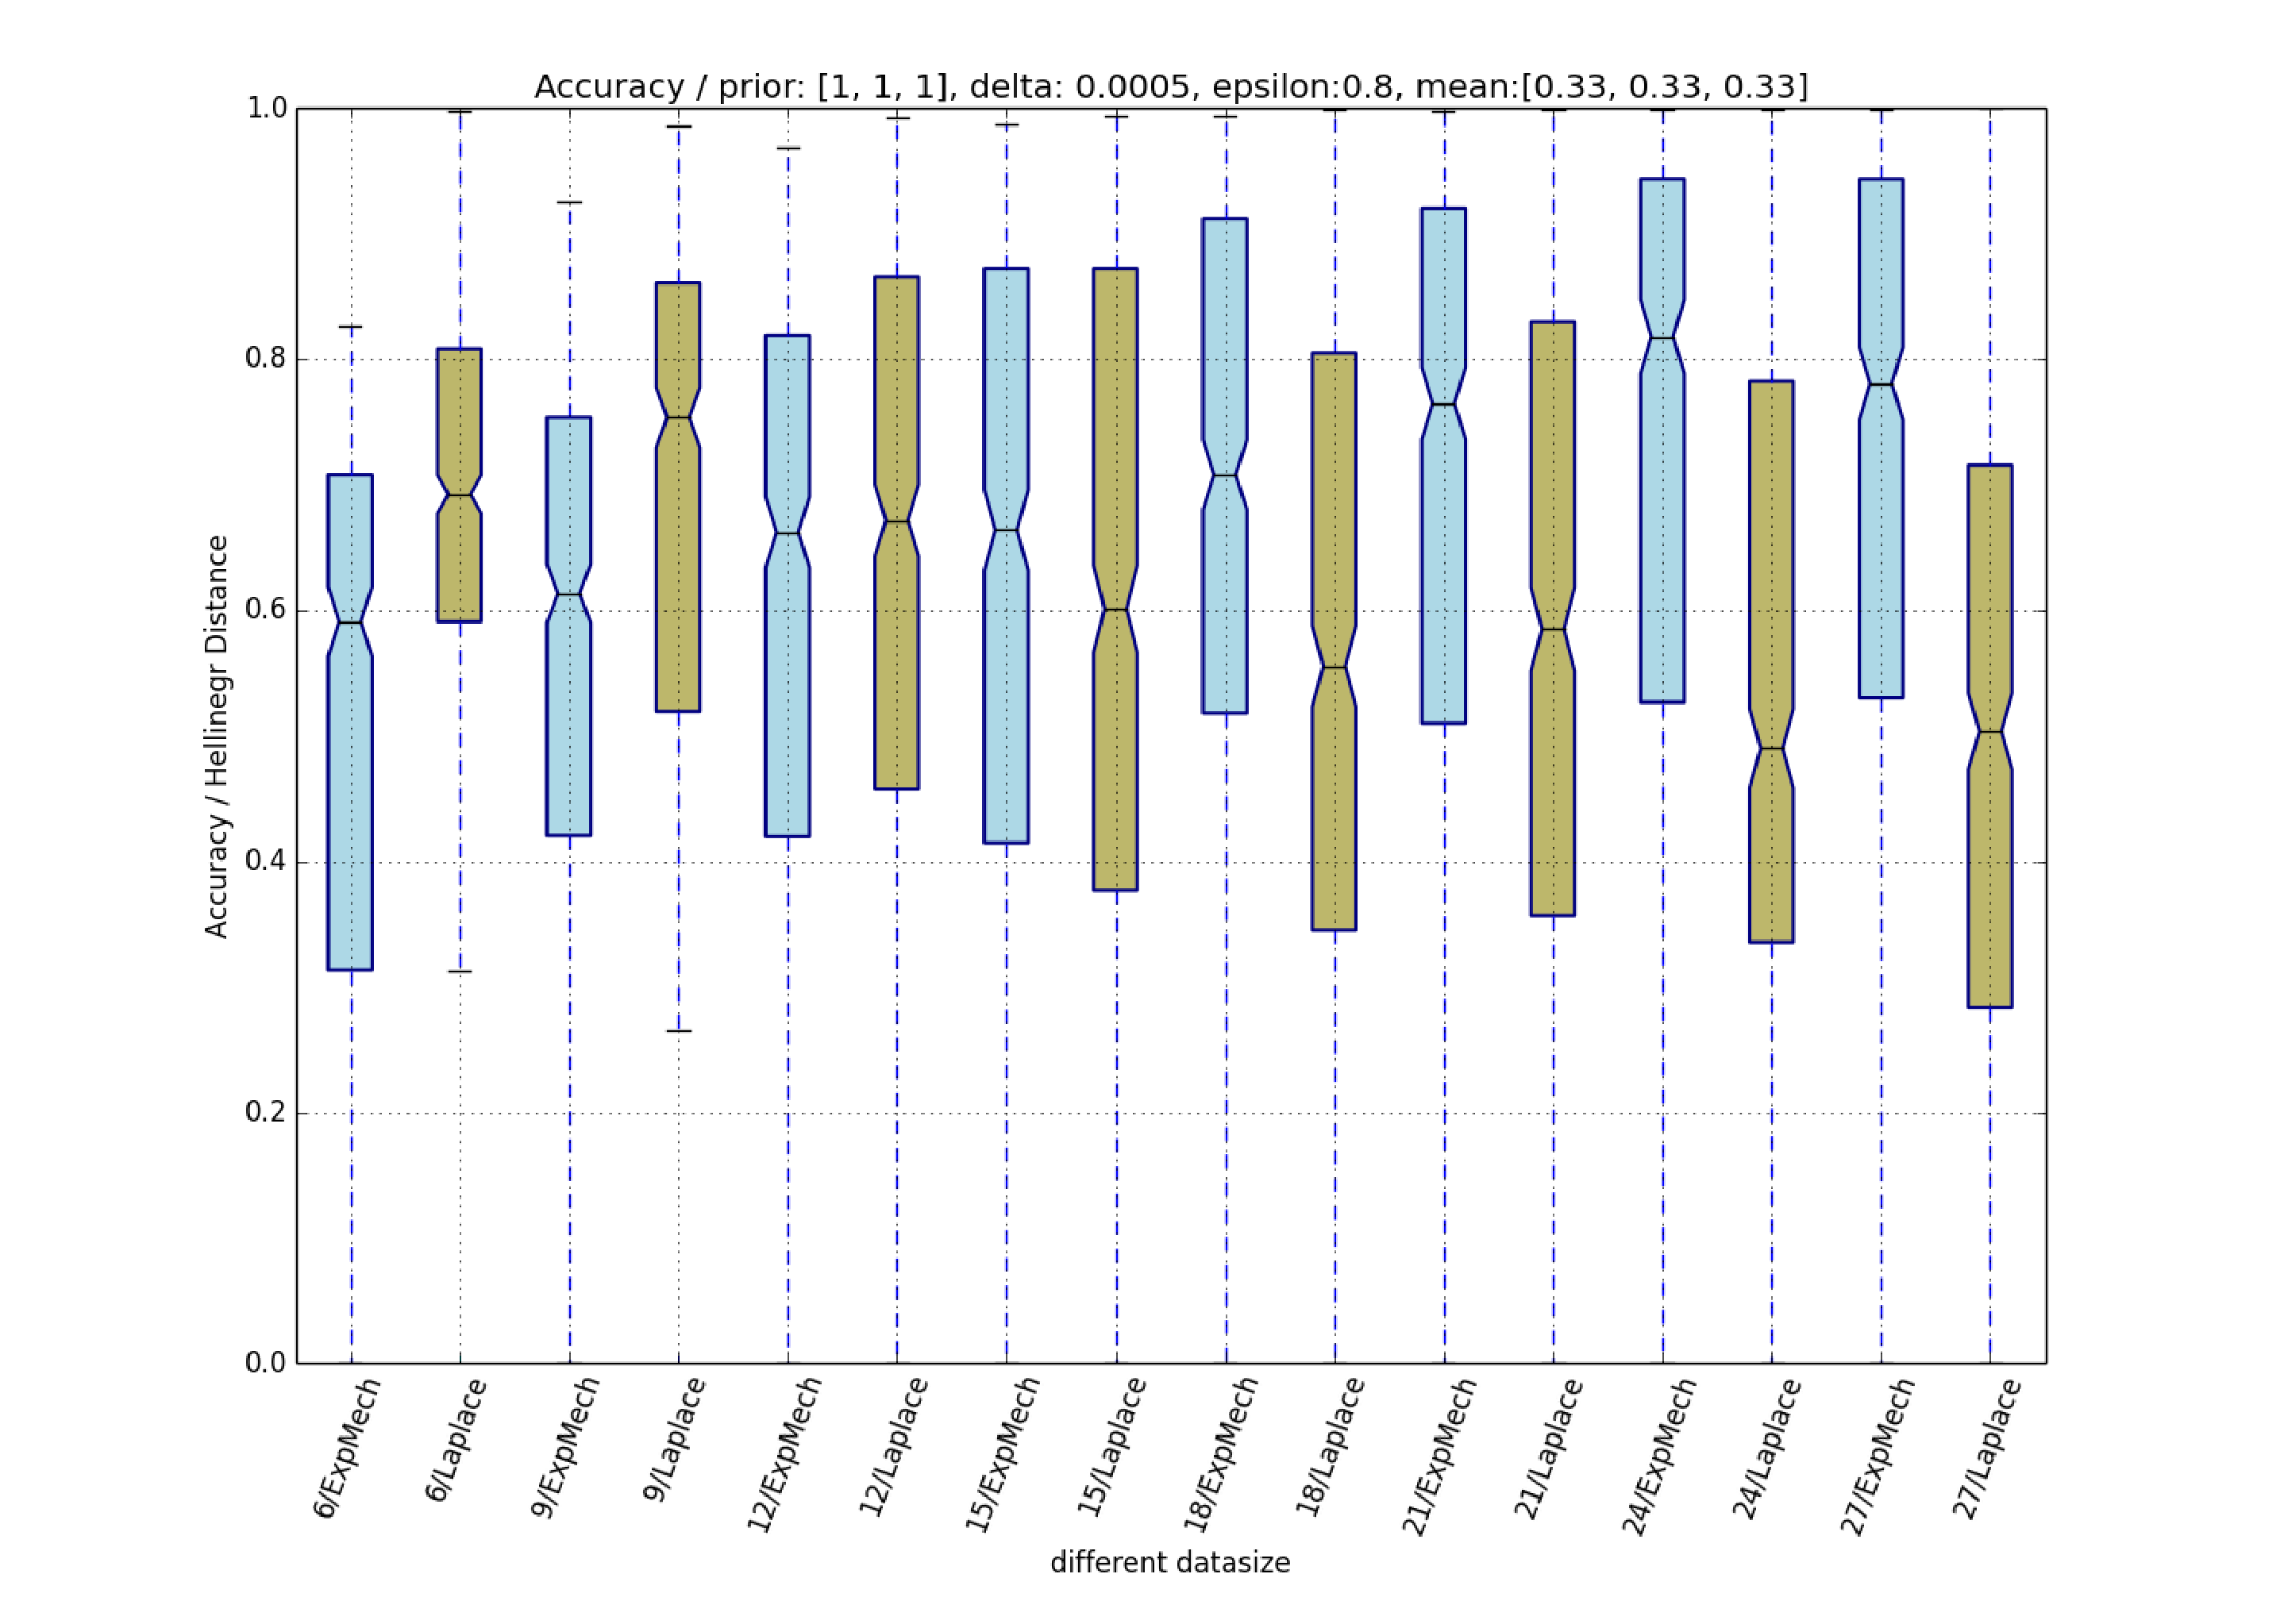
\includegraphics[width=0.3\textwidth]{accuracy_vs_datasize_1_1_1.eps}} 
\caption{Balanced datasets}
\label{fig_vs_datasize}
\end{center}
\end{figure}

In Figure \ref{fig_vs_datasize} we consider \emph{balanced} datasets of observations.
This means that in the Beta-Binomial setting the datasets will be
half 1s and half 0s, while int the Dirichelet-Multinomial the data will be
equally split in all the $k=3$ bins. Figure \ref{fig_vs_datasize} shows that  when the
data size increases, the accuracy of $\hexpmech$ and $\hexpmechd$
decreases. In Figure \ref{fig_vs_datasize}(a), when the data size is
smaller than 12, $\hexpmech$ can outperform the Laplace mechanism but it fails to do so
for bigger datasets. The same happens in as in Figure \ref{fig_vs_datasize}(b):
the Laplace mechanism starts performing better for datasets bigger than 15. 

\paragraph{Increasing dimensions and data size with balanced dataset}
\label{subsubsec_vs_dimension}
In Figure  \ref{fig_vs_dimension}, in the x-axis are observed data sets of
different sizes and different dimensions. The plot shows that increasing the number of dimensions have
a similar pejorative effect on $\hexpmech, \hexpmechd$, and the Laplace
mechanism. Fixing the number of dimensions and increasing the data size shows that
the Laplace mechanism is more accurate then both $\hexpmech$ and $\hexpmechd$. 
In other words, dimensions have little influence on whether our mechanisms will beat the Laplace
mechanism.
\begin{figure}[ht]
\centering
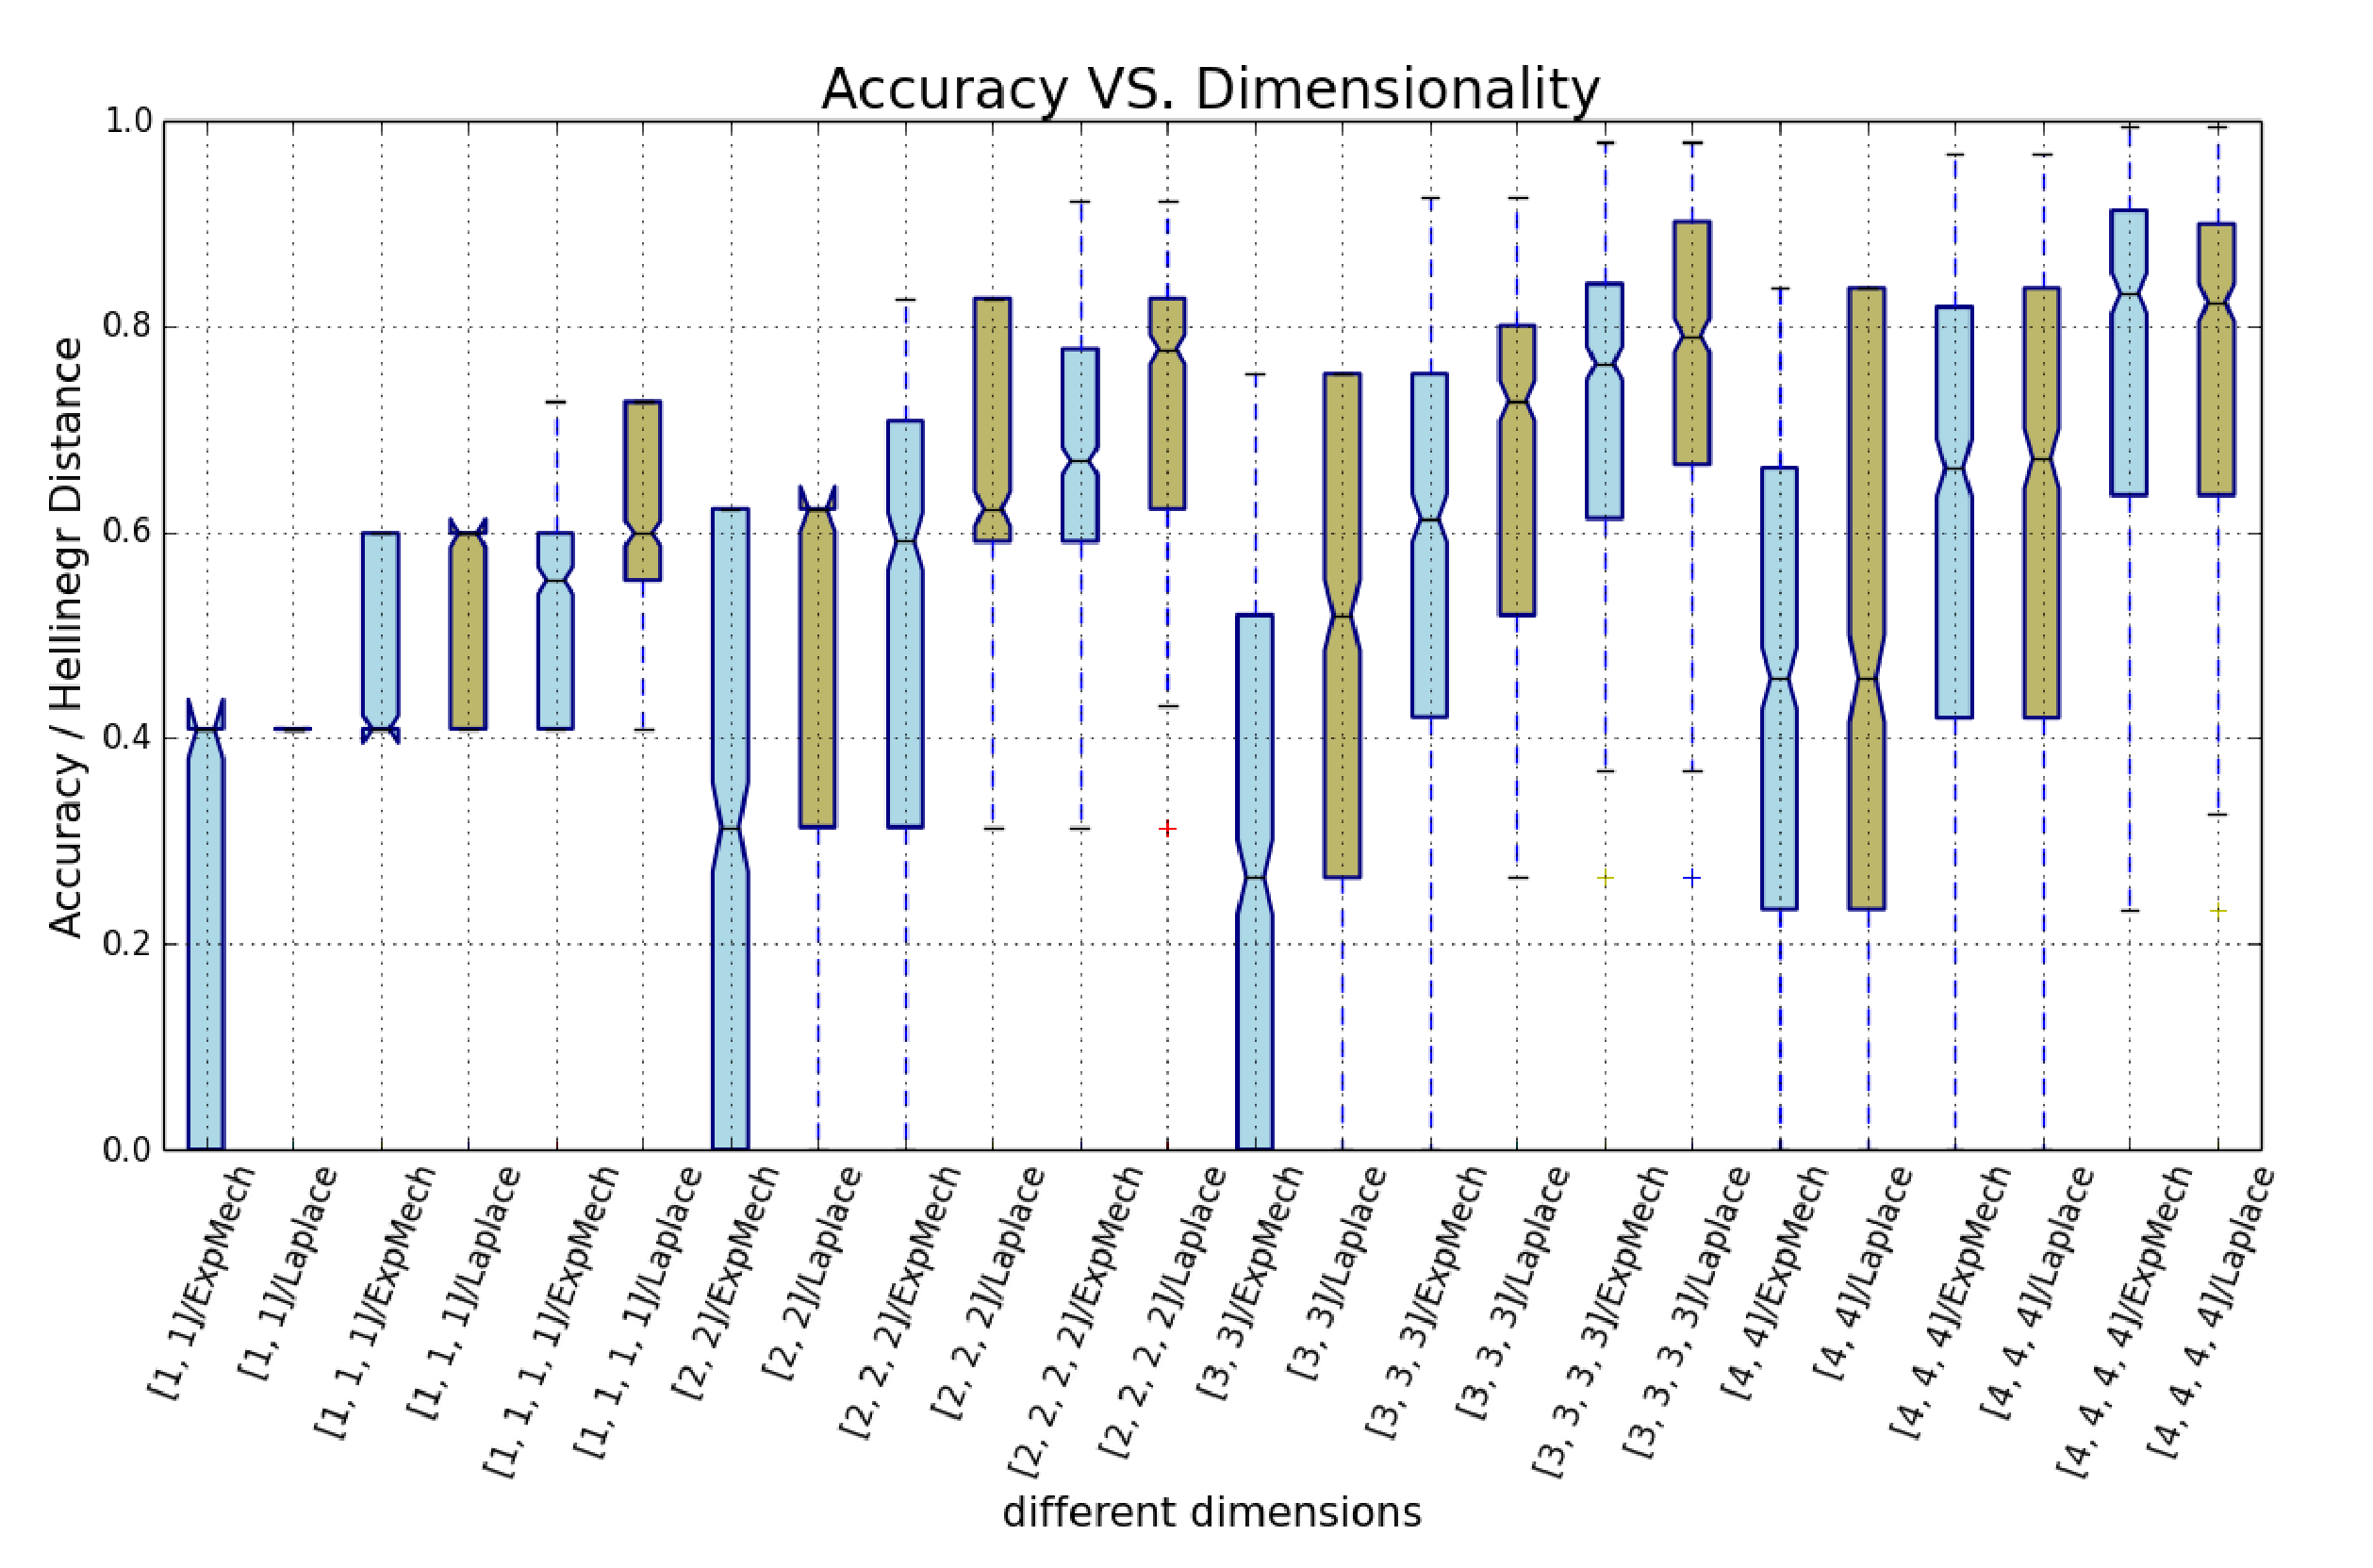
\includegraphics[width=0.45\textwidth]{accuracy_vs_dimension.eps}
\caption{Increasing dimensions and data size with balanced dataset. Priors have 1s in every dimension.}
\label{fig_vs_dimension}
\end{figure}

\paragraph{Fixed data size and unbalaced datasets}
\label{subsubsec_vs_variance}
In Figure \ref{fig_vs_variance}, in the x-axis we considered different levels
of balance of the datasets. We  study this variable only under
two-dimensions $\betad$ distribution in order to be more concise. The plot shows
that $\hexpmech$ accuracy is better than the one of Laplace when the dataset is balanced.

\begin{figure}[ht]
\centering
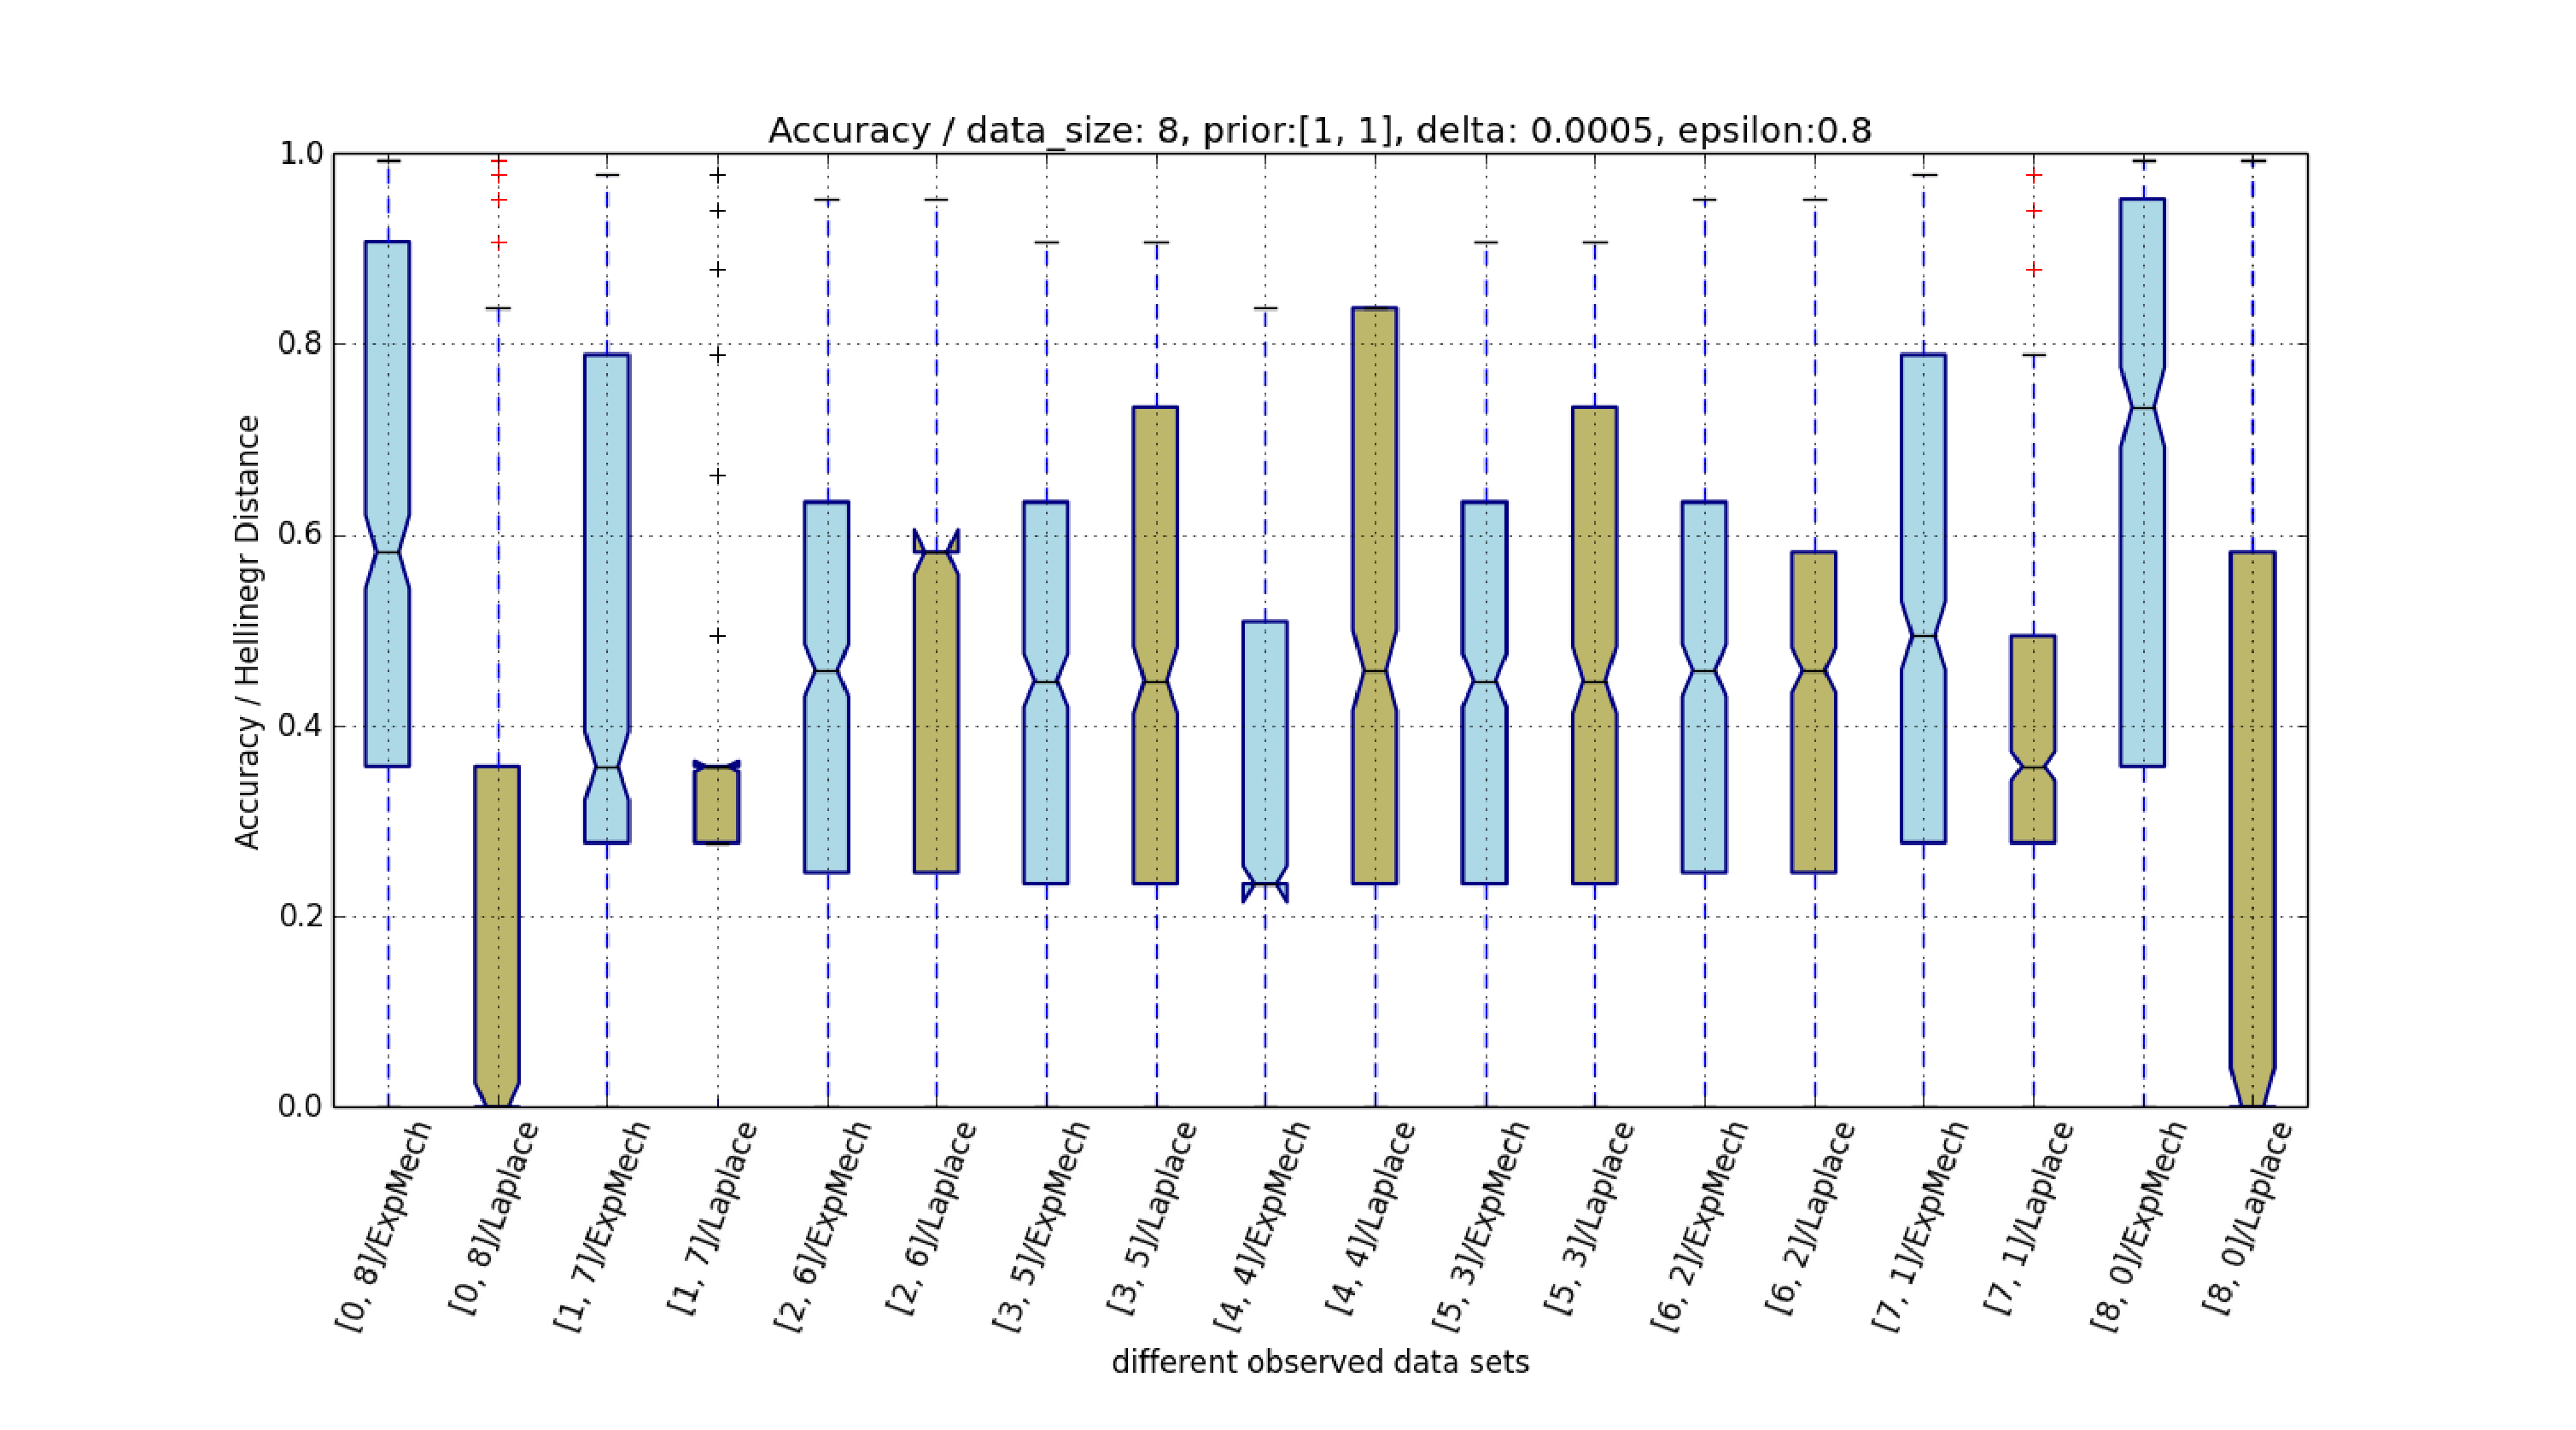
\includegraphics[width=0.45\textwidth]{accuracy_vs_mean_1_1.eps}
\caption{Unbalanced datasets. Prior distributions have 1s in every dimension.}
\label{fig_vs_variance}
\end{figure}




\paragraph{Fixed dataset varying balanced priors}
\label{subsubsec_vs_prior}
In Figure \ref{fig_vs_prior}, we fix the dataset to be $\langle 5,5,5\rangle$.
We also considered balanced priors with increasing values in their dimensions.
The plot shows that in the beginning the Laplace mechanism performs better but
it is outperformed after a while.
\begin{figure}[ht]
\centering
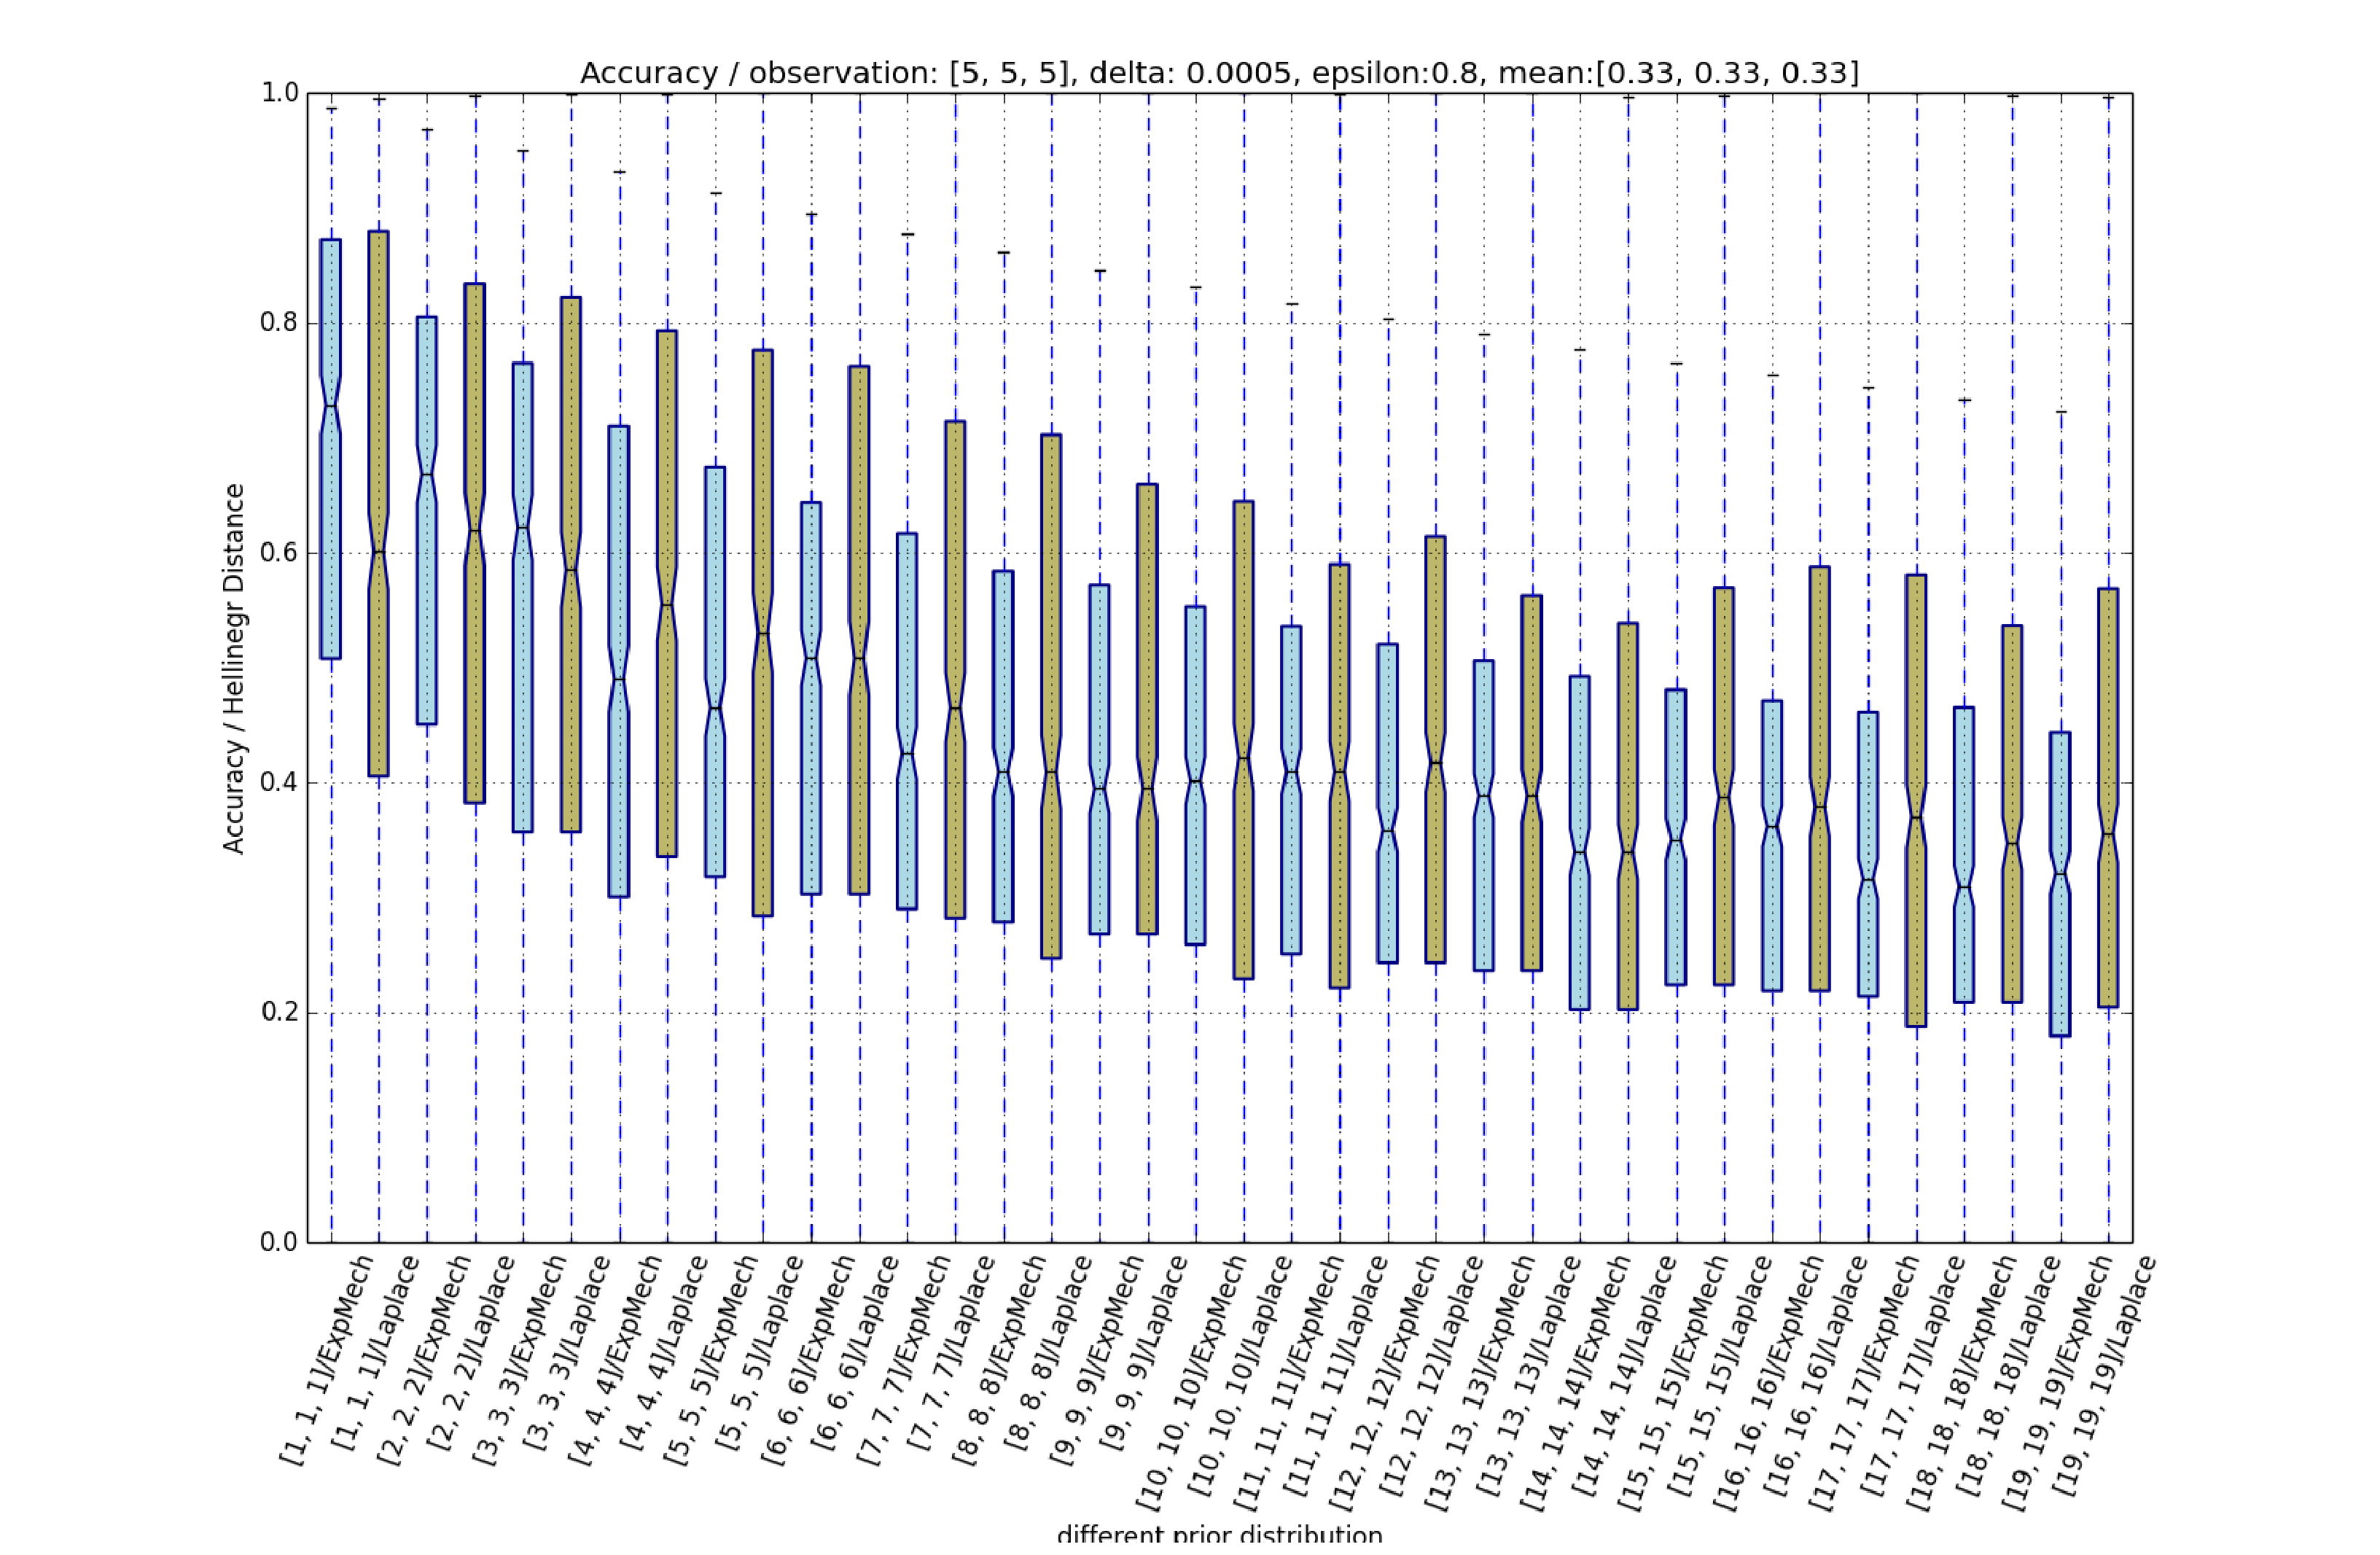
\includegraphics[width=0.45\textwidth]{accuracy_vs_prior_5_5_5.eps}
\caption{Observed data set is: $\langle 5,5,5\rangle$, varying balanced priors}
\label{fig_vs_prior}
\end{figure}





% \subsubsection{Accuracy Evaluation wrt. Prior Distribution and Data Variance}
% \label{subsubsec_vs_prior_variance}

% \begin{figure}[ht]
% \centering
% 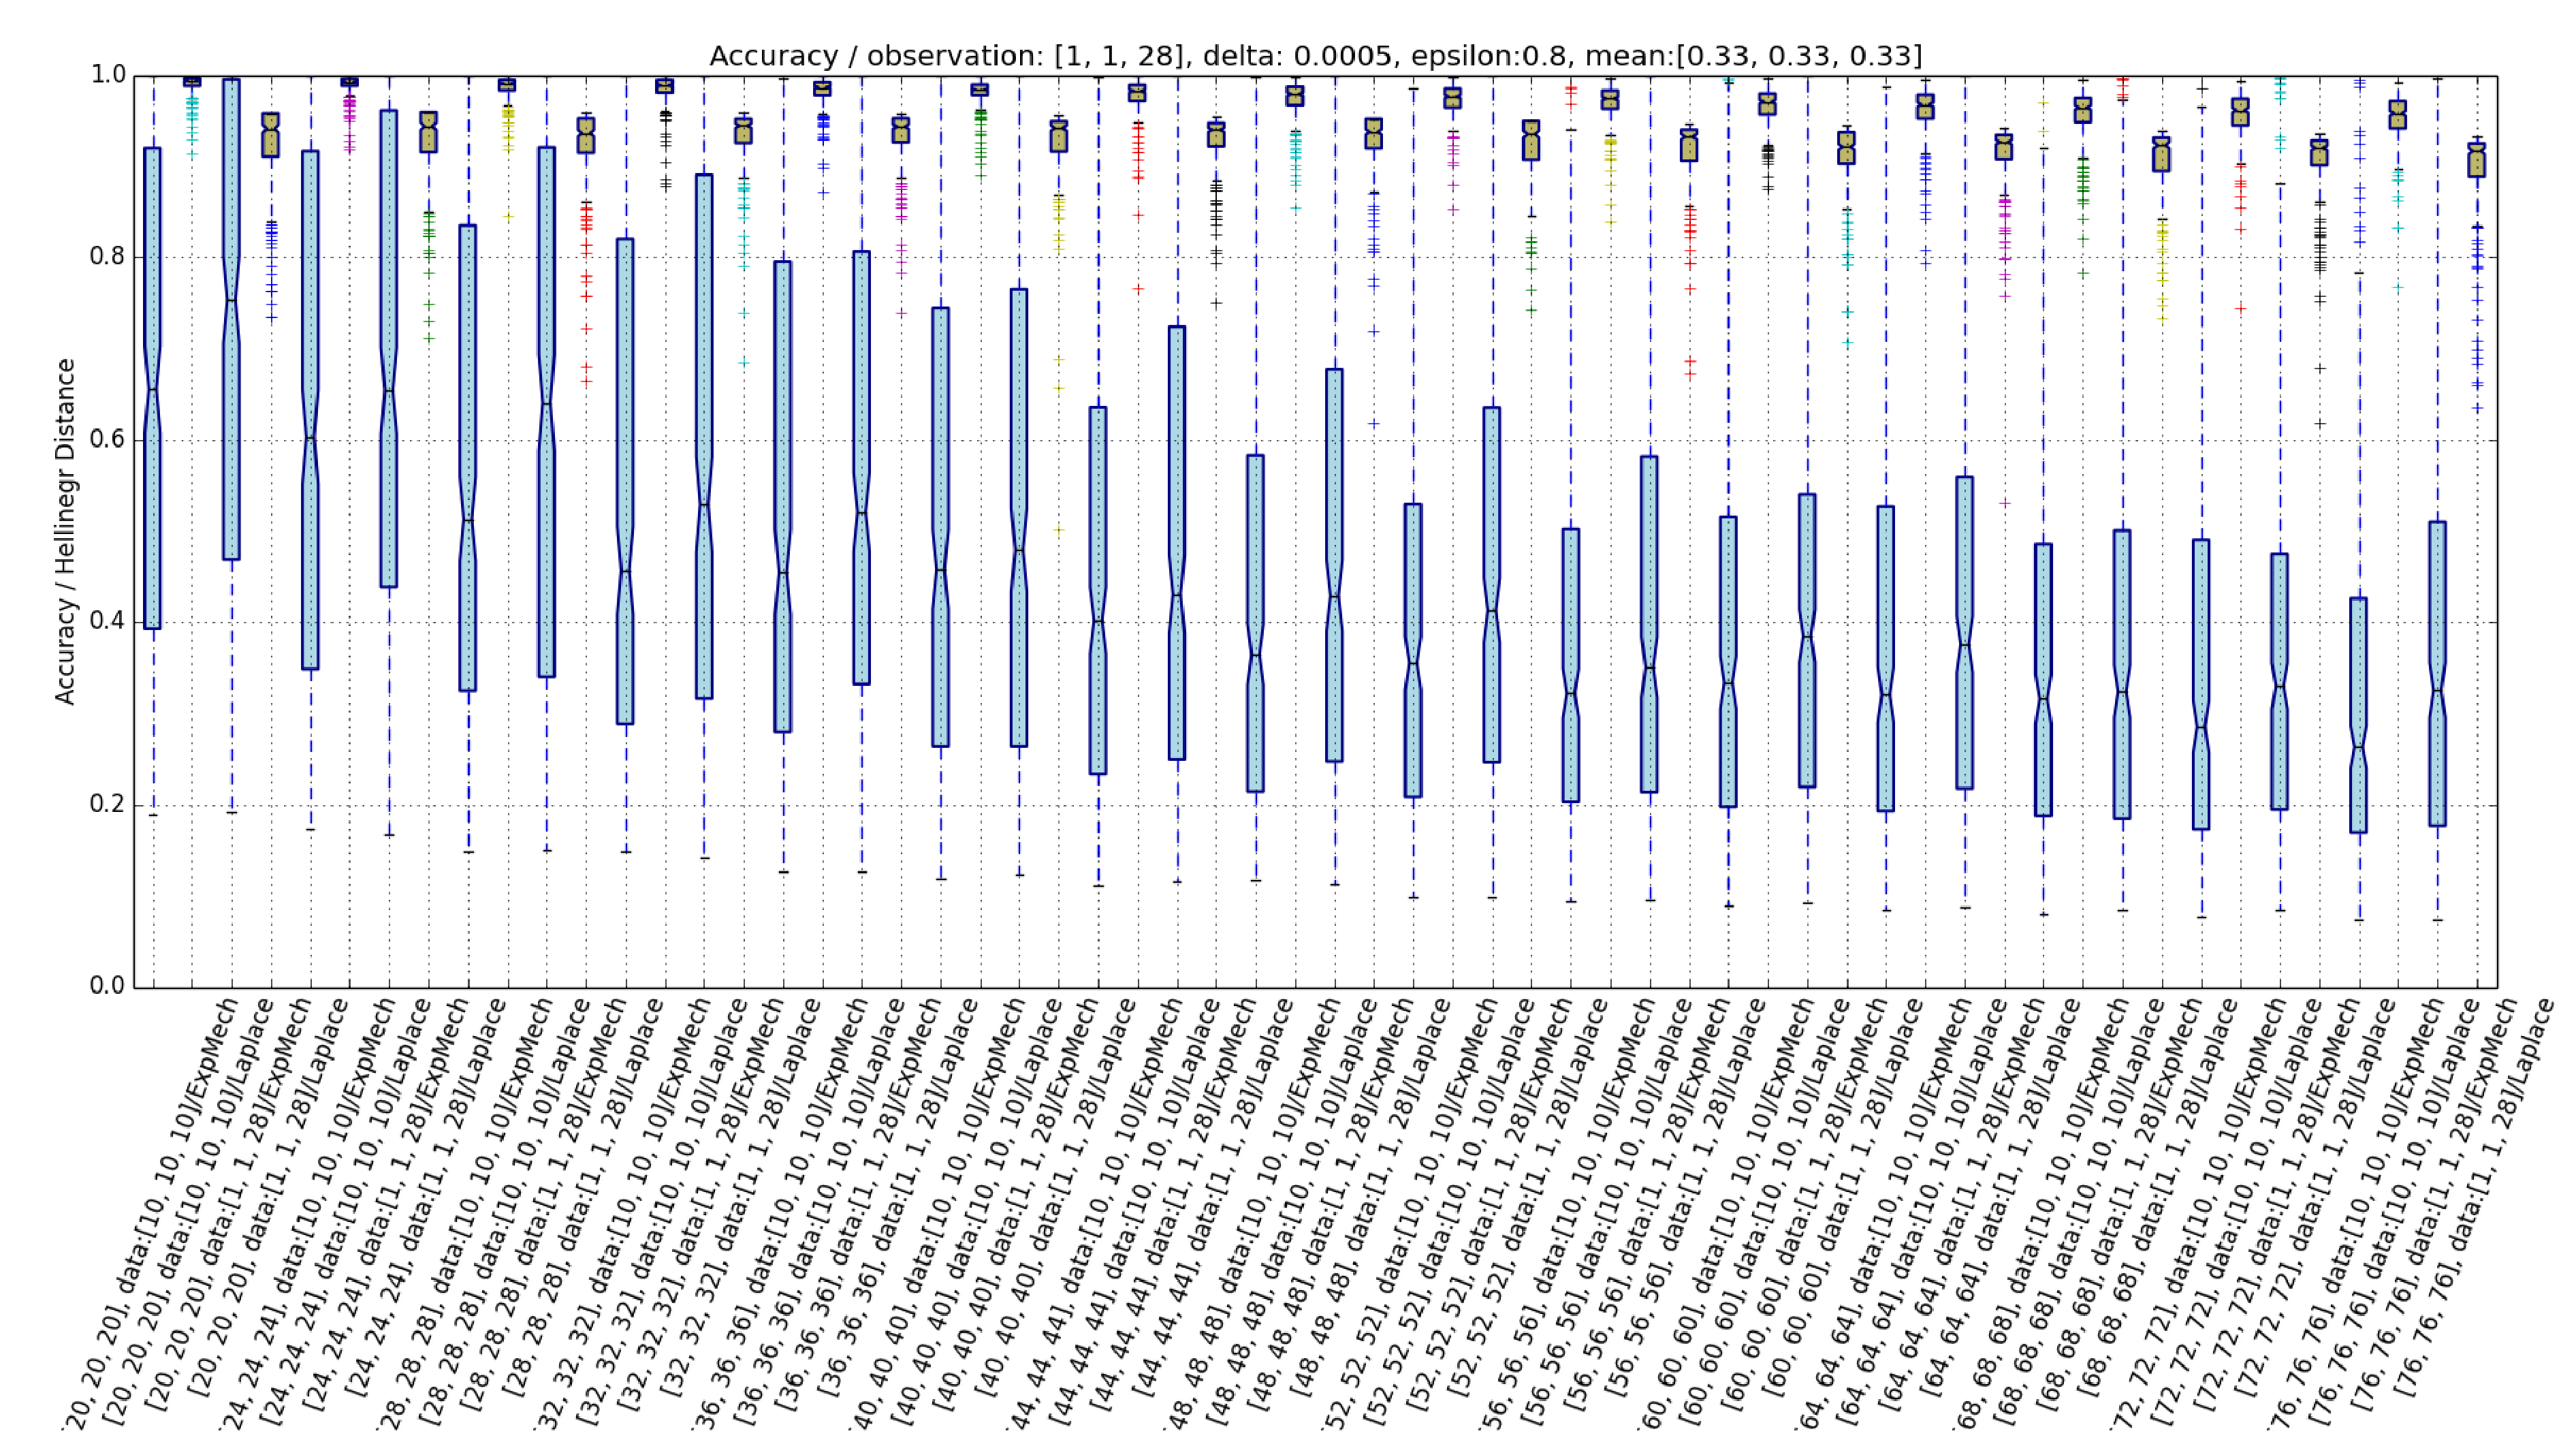
\includegraphics[width=0.45\textwidth]{Accuracy_VS_Prior_mean.eps}
% \caption{Accuracy measurement based on Hellinger distance wrt. different prior distribution and data variances. Settings: $\epsilon = 0.8$ and $\delta = 0.00000001$, observed data sets are $[10,10,10]$ and $[1,1,28]$ and prior distributions are range from $[20,20,20]$ to $[76,76,76]$}
% \label{fig_vs_prior_variance}
% \end{figure}

% Here, we change the prior distribution and data variance in the same time. As shown in Figure  \ref{fig_vs_prior_variance}, our exponential mechanism do better in uniform data set than in edging data set while Laplace mechanism on the contrary. Moreover, our mechanism is improving continuously and significantly as prior distribution increasing while Laplace mechanism isn't.


\section{Conclusions and Future Works}
We can obtain some preliminary conclusions: 
\begin{enumerate}
	\item We can beat Laplace mechanism when data size is small.
	\item We will beat Laplace mechanism when observed data are more uniformly.
  \item When prior distribution grow larger, we perform better and better and beat Laplace mechanism finally.
\end{enumerate} 

In conclusion, this mechanism has better accuracy in small data size, larger prior and uniformly data. But this is not enough for application. We will continue our work in following three directions:
\begin{enumerate}
  \item For now, we just have a intuitive impression on the accuracy behavior of our mechanism, not a precise formula or bound on it.  When we will beat the baseline mechanism and when not? How much influence will elements in experiment section have on the accuracy? Are there any other important factors we missed? These are three problems w.r.t. the accuracy we are going to explore next.
  \item The $(\epsilon, \delta)-$dp is a privacy bound of our exponential mechanism $\hexpmech$ and $\hexpmechd$, but not a tight bound. The real privacy in experiments can be smaller than it. This means we can improve our accuracy in a way that increase the privacy bound but still achieve $(\epsilon, \delta)-$dp. 
  \item Our main idea is that mechanism based on metric over distribution but not numeric. The metric we are using is Hellinger distance here. It is worth to explore other distribution distance metric like KL-divergence and so on.
\end{enumerate}



\bibliographystyle{ACM-Reference-Format}
\bibliography{bayesian.bib}

\end{document}
